\chapter{Le Plan de Lecture de Charge}
    \chapterprecishere{
        ``Potentielle citation sans aucun rapport avec le sujet"\par\raggedleft--- \textup{Personne inconnue}, contexte à déterminer
    }
    
    Dans ce chapitre est présenté le \gls{crp} de \gls{wa105}, pour le prototype 311 et pour le démonstrateur 666, ainsi que les études et mesures relatives au \gls{crp} faites durant cette thèse.
    
    Sauf indication contraire, les caractéristiques décrites dans ce chapitre sont identiques pour le démonstrateur 666 et pour le prototype 311.
    
    
    \section{Introduction technique}
        
        Dans cette section sont présentées les différentes parties du \gls{crp}. La première sous-section sert d'introduction générale, puis une sous-section est dédié chaque élément important du \gls{crp}.
        
        \subsection{Rôle du CRP}\label{sec::crp_intro}
            \begin{figure}[htbp]
                \begin{center}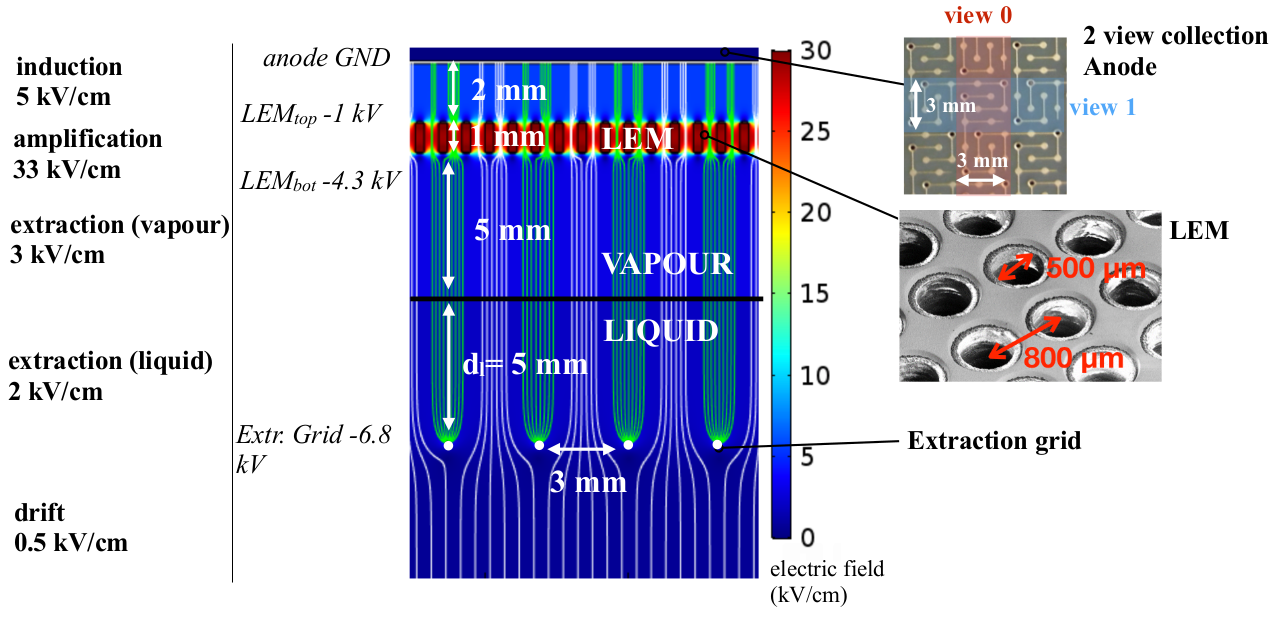
\includegraphics[width=\textwidth,keepaspectratio]{crp_fields.png}\end{center}
                \caption[Champs électriques d'un  \gls{crp}.]{Illustration des trois principales zones d'un \gls{crp} de \gls{dlartpc}. Les champs et potentiels électriques indiqués correspondent à l'exploitation réussie d'une \gls{dlartpc} ayant atteint des gains effectifs de l'ordre de 20 \cite{Aimard2018,Cantini2014}.}
                \label{fig::crp_fields}
            \end{figure}
            \begin{figure}[htbp]
                \begin{subfigure}[b]{\textwidth}
                    \begin{center}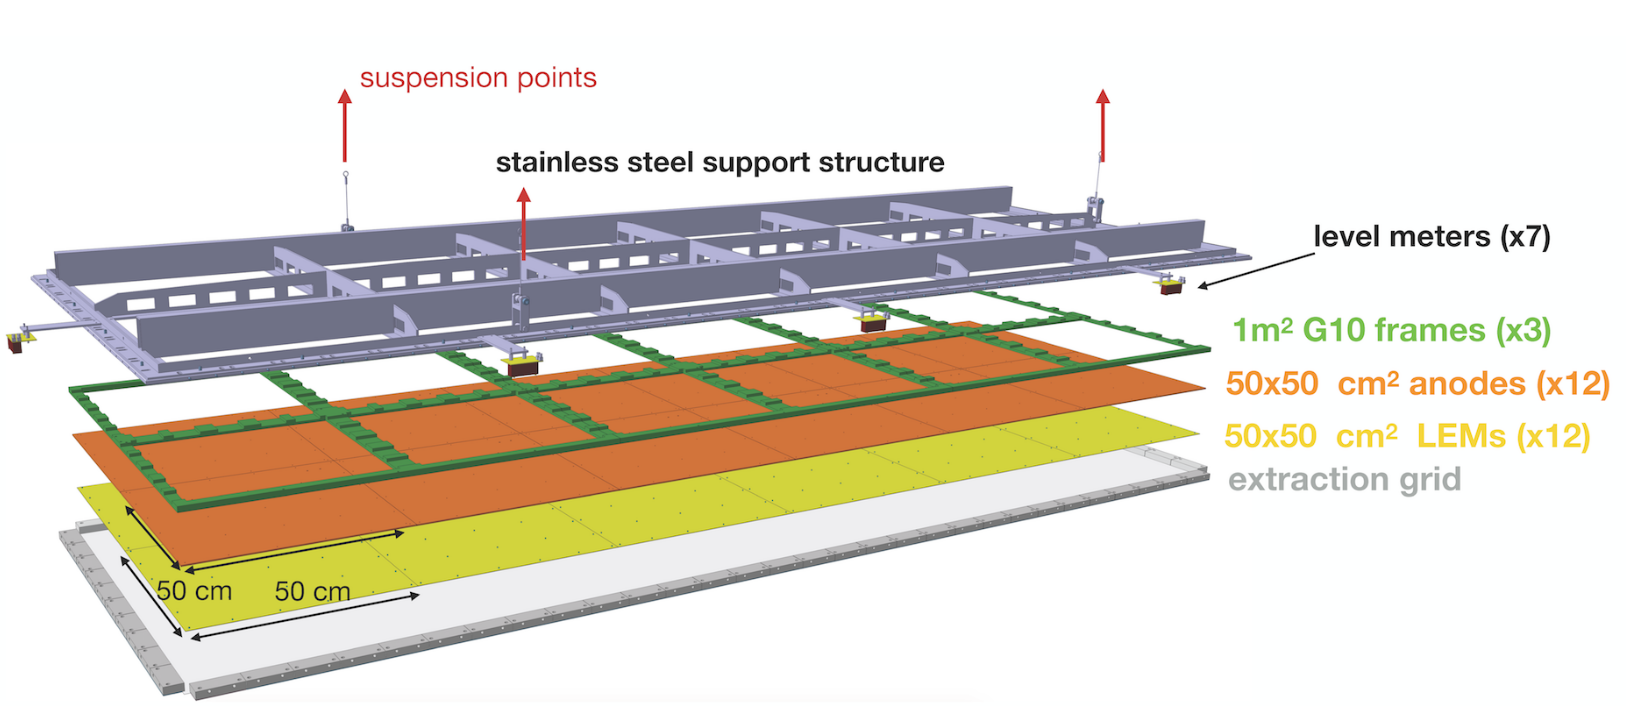
\includegraphics[width=\textwidth,keepaspectratio]{crp_311.png}\end{center}
                    \caption[\gls{crp} du prototype 311]{Schéma explosé du \gls{crp} du prototype 311. Les flèches rouges représentent les câbles de suspensions \cite{Aimard2018}.}
                    \label{fig::crp_311}
                \end{subfigure}
                \begin{subfigure}[b]{\textwidth}
                    \begin{center}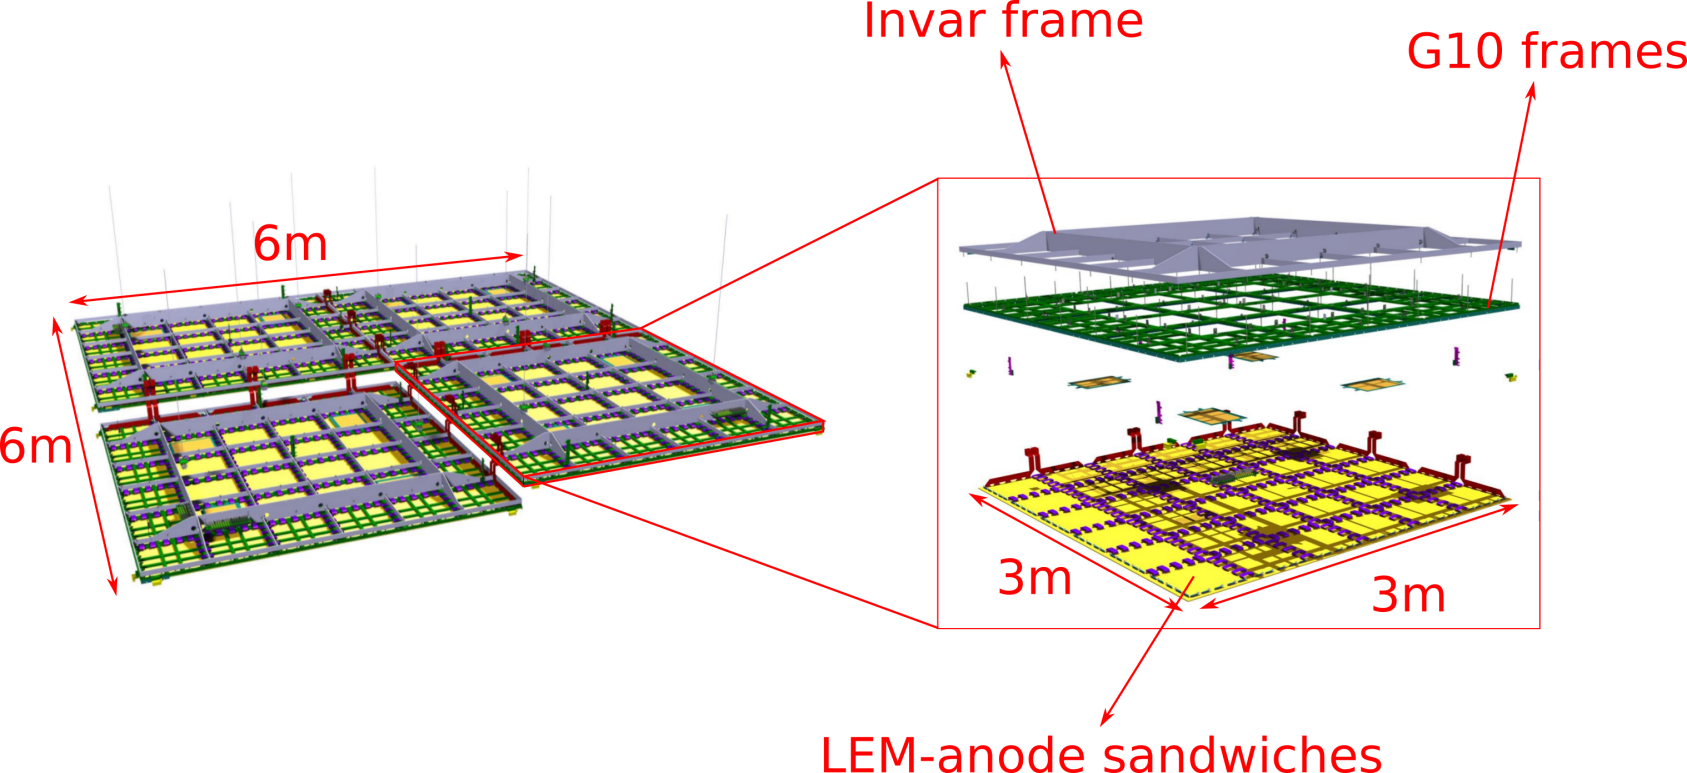
\includegraphics[width=\textwidth,keepaspectratio]{crp_666_complete.png}\end{center}
                    \caption[\glspl{crp} du démonstrateur 666]{Schéma des \glspl{crp} du démonstrateur 666. L'un d'eux est représenté plus bas pour illustrer le fait qu'il y a 4 \glspl{crp}. Chacun mesure $3\times\SI{3}{\meter\squared}$. Les trais gris verticaux représentent les câbles de suspensions. La grille d'extraction n'est pas représentée sur ce schéma. \cite{CRPdesign}}
                    \label{fig::crp_666}
                \end{subfigure}
                \caption{Schéma des \gls{crp} de \gls{wa105}}
            \end{figure}
        
            Le \gls{crp} a pour rôle:
            \begin{enumerate}
                \item L'extraction depuis l'argon liquide vers l'argon gazeux des électrons primaires, issue de l'interaction des particules chargées dans le liquide, après dérive
                \item L'amplification de ces électrons
                \item La collecte du signal ainsi créé
            \end{enumerate}
            Toutes ces étapes sont réalisées grâce à trois champs électriques différents:
            \begin{enumerate}
                \item Le champ d'extraction, créé par une différence de potentielle entre une grille d'extraction et le bas du dispositif d'amplification
                \item Le champ d'amplification, créé par une différence de potentielle à travers le dispositif d'amplification
                \item Le champ d'induction, créé par un différence de potentiel entre le haut du dispositif d'amplification et les anodes de lecture
            \end{enumerate}
            La \autoref{fig::crp_fields} résume les points suivants : la grille d'extraction se situe $\SI{5}{\milli\meter}$ sous le niveau d'argon liquide, le bas du dispositif d'amplification se situe $\SI{5}{\milli\meter}$ au dessus du liquide. La tension appliquée entre les deux de $\SI{2.5}{\kilo\volt}$ correspondant à un champ électrique dans le liquide de $\SI{2}{\kilo\volt\per\centi\meter}$ ($\SI{3}{\kilo\volt\per\centi\meter}$ dans le gaz). Une étude \cite{guschin} a montré qu'à ces tensions, la totalité des électrons peut être extraite du liquide vers le gaz.
            
            Le dispositif d'amplification est un ensemble de plusieurs \glspl{lem}, décrits en détails en \autoref{sec::LEM}, d'une épaisseur de $\SI{1}{\milli\meter}$ à travers laquelle est appliquée une tension de $\SI{3.5}{\kilo\volt}$, correspondant à un champ électrique d'environ $\SI{35}{\kilo\volt\per\centi\meter}$. De précédentes expériences \cite{Badertscher2011,Cantini2014} ont montré qu'un gain de l'ordre de 20 est atteignable à cette tension.
            
            Les anodes, décrites en \autoref{sec::anode}, sont situées $\SI{2}{\milli\meter}$ au dessus des \glspl{lem}. Une tension de $\SI{1}{\kilo\volt}$ entre les anodes et le haut des \glspl{lem} créé un champ d'induction de $\SI{5}{\kilo\volt\per\centi\meter}$, qui doit alors correspondre à un probabilité de collection de charge optimale (voir \autoref{sec::efficacites}).
            
            Les \glspl{lem} et anodes sont fixés sous des supports en fibre de verre G10, eux même fixés sous un squelette en acier inoxydable pour le prototype 311 ou en Invar pour le démonstrateur 666 (voir \autoref{sec::crp_structure}). La grille d'extraction est constituée de fils d'acier inoxydable, chacun tendu à $\SI{1.5}{\newton}$ à température ambiante sur des \glspl{pcb}, eux même fixés sur les bords des supports en G10. Le \gls{crp} est désolidarisé du reste du cryostat, il est donc possible de l'assembler et de le tester à part. Un système de câbles et poulies permet d'ajuster la position du \gls{crp} au dessus du liquide. La \autoref{fig::crp_311} et la \autoref{fig::crp_666} montrent respectivement le \gls{crp} du prototype 311 et un \gls{crp} du démonstrateur 666. Le prototype 311 n'a qu'un \gls{crp} recouvrant toute sa surface, mais le démonstrateur 666 a quatre \gls{crp} de $3\times\SI{3}{\meter\squared}$, indépendants entre eux. Due à des retards de production, seuls deux de ces \gls{crp} sont instrumentés. Sur les deux autres, les \glspl{lem} et anodes ont été remplacés par des \gls{pcb} mis à la masse.
            
            Le \gls{crp} est munie de plusieurs capteurs de pression, de température ainsi que de niveau d'argon liquide afin de suivre en direct les conditions à l'intérieur du détecteur et de pouvoir ajuster le niveau du \gls{crp} par rapport au liquide.
        
        \subsection{Les contraintes techniques et la structure}\label{sec::crp_structure}
            
            Le \gls{crp} doit respecter plusieurs contraintes techniques \cite{CRPdesign} pour permettre une lecture efficace et fidèle de la charge:
            
            \begin{itemize}
                \item Il doit être le plus plat possible, afin que l'interface liquide-gaz si situe bien au milieu de la distance grille--\gls{lem} pour tout le \gls{crp}. La tolérance fixée pour le démonstrateur 666 est de \SI{0.5}{\milli\meter}(TODO: 311?)
                \item Il doit supporter des variations de température importante sans se déformer de manière significative : le \gls{crp} est assemblé à température ambiante et descend ensuite à mois de \SI{90}{\kelvin}
                \item Il doit être possible d'ajuster la position du \gls{crp} par rapport au niveau d'argon liquide à \SI{0.05}{\milli\meter} près.
                \item Le démonstrateur 666 est constitué de 4 \gls{crp}. La distance entre eux doit être de \SI{10}{\milli\meter} maximum
                \item Comme le \gls{crp} est assemblé à part du reste du détecteur, il doit être transportable
                \item Le \gls{crp} du démonstrateur 666 doit être un élément utilisable dans la future expérience \gls{dune}, dont un module de détection sera constitué d'une trentaine de ces \gls{crp}
            \end{itemize}
            
            Afin de satisfaire ces contraintes, la structure principale des \glspl{crp} du démonstrateur 666 est faite en Invar, un alliage de fer et de nickel dont le coefficient de dilatation thermique est particulièrement faible (\SI{1.5e-6}{\per\kelvin} entre \SI{22}{\celsius} et \SI{-186}{\celsius}). La structure du \gls{crp} du prototype 311 est elle faite en acier inoxydable.
            
            Les \glspl{lem} et anodes sont montés sur des cadres en G10 (neuf dans le 666 et trois dans le 311), de la fibre de verre feuilletée solide et électriquement isolante(TODO trouver des chiffres). Des mesures de contraction thermique réalisées en 2015 ont donné pour le G10 utilisé dans \gls{wa105} des coefficients de l'ordre de \SI{e-5}{\per\kelvin}, proches du ceux des \glspl{las}. Le G10 et les \glspl{las} réagissent donc de la même manière aux différents changements de température. Sur les trois mètres du \gls{crp} du démonstrateur 666, la contraction maximum mesurée est d'environ \SI{6}{\milli\meter}. L'Invar se contractant beaucoup moins, les cadres en G10 sont fixés sur la structure en Invar avec des éléments permettant au G10 de se contracter librement.
            
            Le positionnement vertical et horizontal des \glspl{crp} se fait grâce à un système de suspension. Un \gls{crp} (dans le 666 comme dans le 311) est suspendu par trois câbles motorisés, passant par des conduites isolantes traversant le couvercle du détecteur pour atteindre le \gls{crp}. Ils permettent une amplitude verticale de \SI{98}{\milli\meter} dans le démonstrateur 666 (\SI{40}{\milli\meter} dans le prototype 311) avec une précision de \SI{100}{\micro\meter} et une amplitude horizontale de \SI{26}{\milli\meter} dans le démonstrateur 666. Le 311 n'est pas pourvu d'un système de positionnement horizontal.
            
            Les \glspl{las} sont assemblés et fixés sur le cadre en G10 par des entretoises en PEEK (polyétheréthercétone) assurant l'espacement de \SI{2}{\milli\meter} entre les \glspl{lem} et les anodes. Les extrémités de ces entretoises sont filetées, un côté est vissé directement dans le G10.
            
        \subsection{Électronique : signaux, alimentation}
            
            Les signaux sont apportés vers l'extérieur par des conduites similaires à celles des câbles de suspension, remplies d'azote \cite{Acciarri2016a} traversant le couvercle du détecteur. Elles sont faites de manière à ce que l'électronique Frontend soit accessible pour d'éventuelles réparations sans contaminer l'argon. Les cartes Frontend (des circuits CMOS ASIC) sont située en bas des conduites et refroidie à \SI{110}{\kelvin}. L'électronique numérique et le \gls{daq} sont situés en dehors du cryostat.
            
            L'alimentation haute tension passe elle aussi par des conduites isolante, et est distribuée aux \gls{lem}, aux anodes et à la grille d'extraction par des câbles coaxiaux courant le long de la structure du \gls{crp}. Dans le prototype 311, chaque face de chaque \gls{lem} ainsi que chaque anode a sa propre alimentation. Dans le démonstrateur 666, les faces hautes des \gls{lem} sont alimentées par groupe de six.
            
            Les anodes sont reliées entre elles via des nappes et des connecteurs KEL formant des canaux de trois mètres de long dans le 666 et trois ou un mètre dans le 311.
            
        \subsection{Les anodes}\label{sec::anode}
        
            \begin{figure}[htbp]
                \begin{center}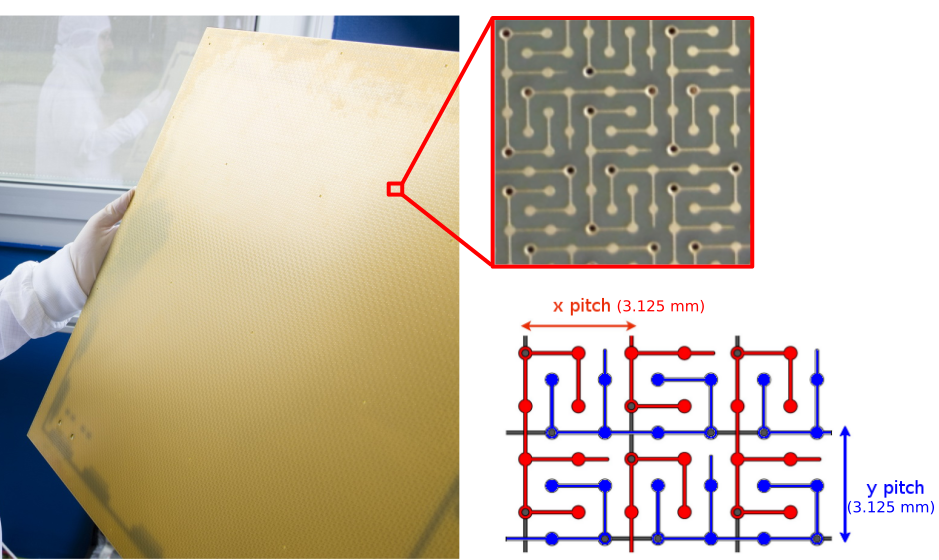
\includegraphics[width=\textwidth,keepaspectratio]{anode.png}\end{center}
                \caption[Agrandissement d'une anode de lecture.]{Agrandissement d'une anode de lecture. L'orthogonalité des pistes des vues $x$ et $y$ facilite la reconstruction des événements, la dispositions en plusieurs couches assure une capacitance de $\SI{160}{\pico\farad\per\meter}$ \cite{Cantini2013}.}
                \label{fig::anode}
            \end{figure}
            \begin{figure}[htbp]
                \begin{center}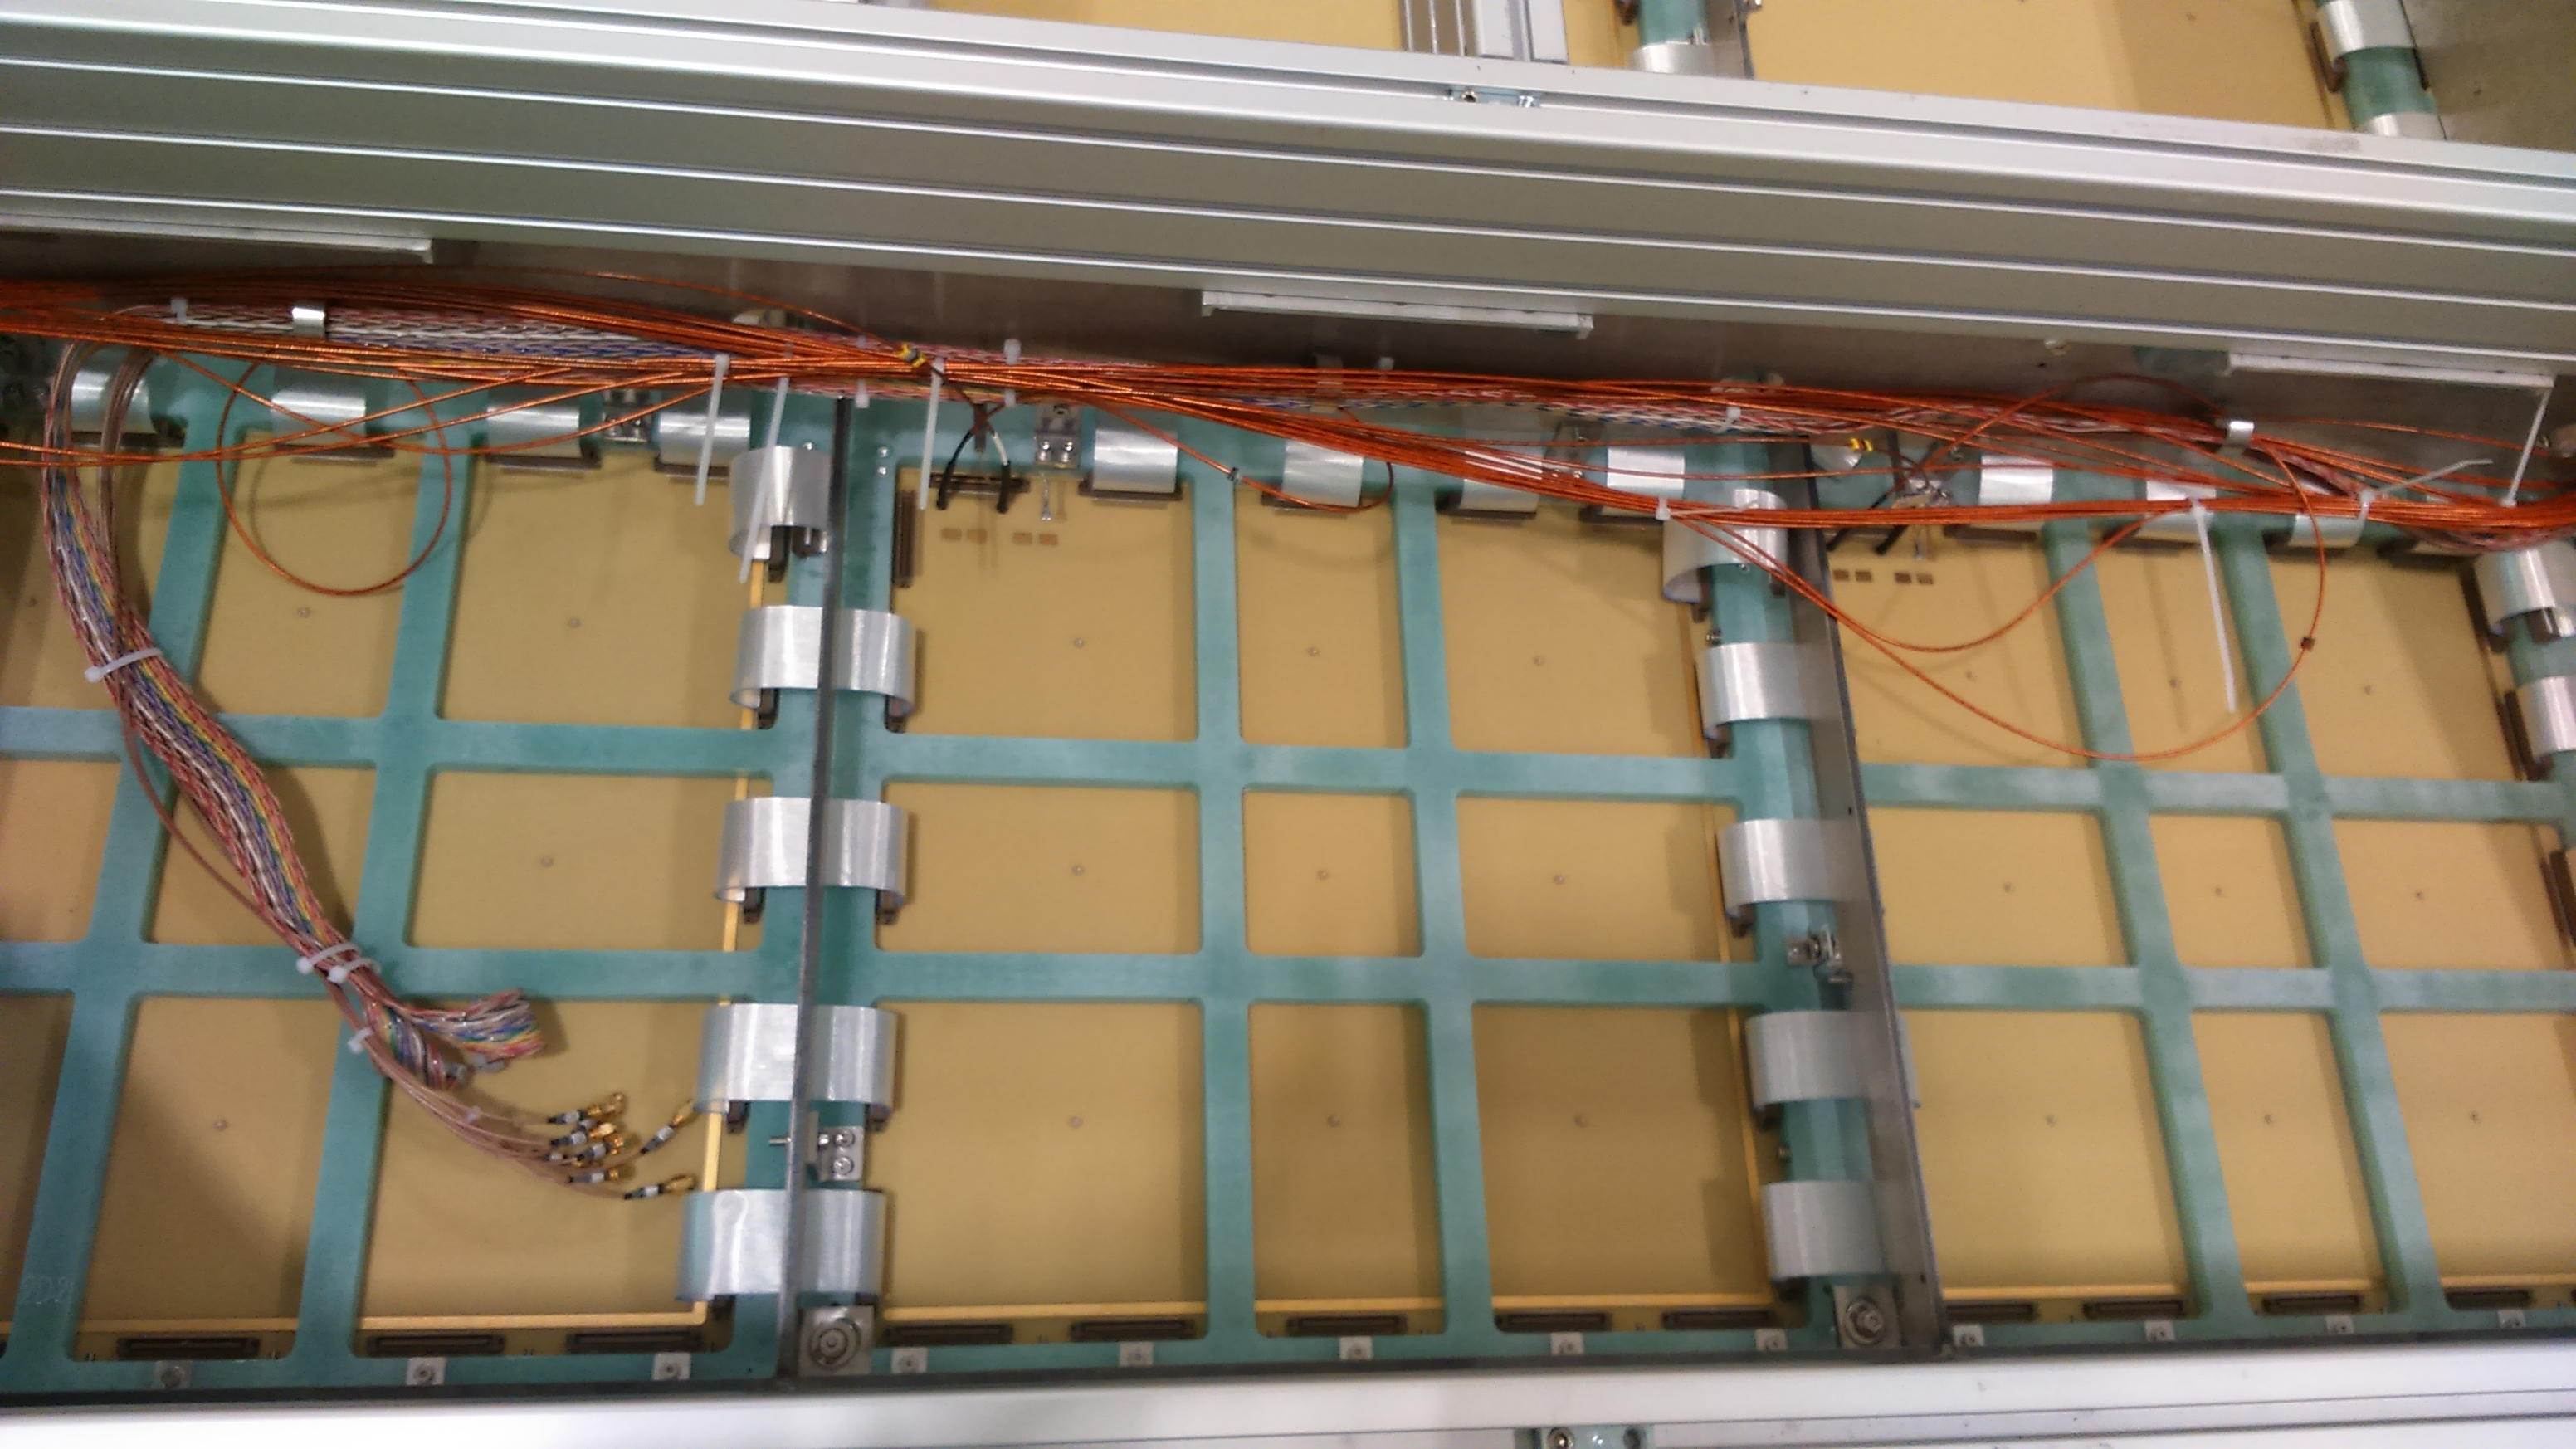
\includegraphics[width=\textwidth,keepaspectratio]{connecteurs2.JPG}\end{center}
                \caption[Vue du dessus d'un \gls{crp} du démonstrateur 666.]{Vue du dessus d'un \gls{crp} du démonstrateur 666. On peut y voir les câbles d'alimentation haute tension des \glspl{lem} le long de la structure en Invar ainsi que les nappes reliant les connecteurs KEL entre les anodes, formant des canaux de \SI{3}{\meter}.}
                \label{fig::connecteurs}
            \end{figure}
            
            Le modèle des anodes, fabriquées par la compagnie ELTOS\footnote{\url{http://www.eltos.com/en/}} en Italie, est le résultat de tests réalisés au CERN par l'\gls{ethz} dans un prototype de \gls{dlartpc} de $\SI{3}{\liter}$ \cite{Cantini2013} en vue de réduire au maximum la capacitance, et donc le bruit, tout en ayant un partage égale de charge entre deux vues perpendiculaires, facilitant la reconstruction des événements et leur analyse.
            
            Chaque anode est un PCB de quatre couches, avec une surface de  $50\times\SI{50}{\centi\meter\squared}$ et comporte deux jeux de canaux perpendiculaires, \numprint{160} pour la vue $x$ et \numprint{160} pour la vue $y$. La \autoref{fig::anode} montre un agrandissement de la surface active d'une anode. La largeur d'un canal est de $\SI{3.125}{\milli\meter}$ et correspond à deux lignes inter-connectées, de cuivre recouvertes d'or. Les canaux sont ramenés par groupes de 32 vers l'autre surface de l'anode jusqu'à des connecteurs KEL de 68 pins, dont les 36 pins restant sont mis à la masse. Dans le prototype 311 comme dans le démonstrateur 666, ces connecteurs sont reliés entre eux d'une anode à l'autre afin de former des canaux continus de $\SI{1}{\meter}$, $\SI{3}{\meter}$ ou $\SI{6}{\meter}$ (voir  \autoref{fig::connecteurs}). La capacitance linéique est alors de $\SI{160}{\pico\farad\per\meter}$, correspondant à un bruit de fond équivalent à 1400 électrons \cite{Aimard2018} pour les longs canaux de $\SI{3}{\meter}$ du prototype 311.
            
            Les anodes ont été inspectées visuellement par le fabricant avant envoie, et la continuité de leurs canaux a été testée par Saclay (plus de détails en \autoref{sec::test_anode}).
        
        \subsection{Les Large Electron Multipliers (LEM)}\label{sec::LEM}
            
            \begin{figure}[htbp]
                \begin{center}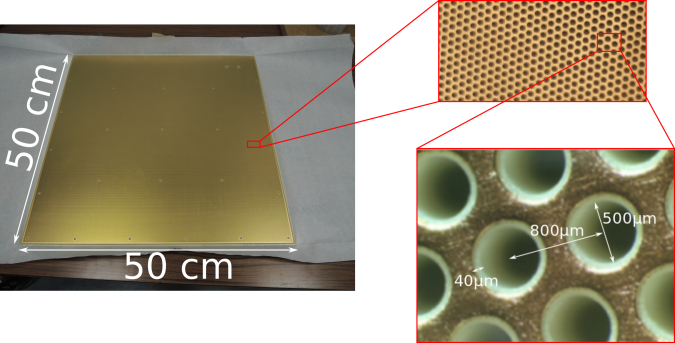
\includegraphics[width=\textwidth,keepaspectratio]{LEM_zoom.png}\end{center}
                \caption[Photo d'un \gls{lem}.]{Photo d'un \gls{lem} avec agrandissement de la disposition en nid d'abeille des trous d'amplification.}
                \label{fig::LEM}
            \end{figure}
            \begin{figure}[htbp]
                \begin{subfigure}[t]{0.48\textwidth}
                    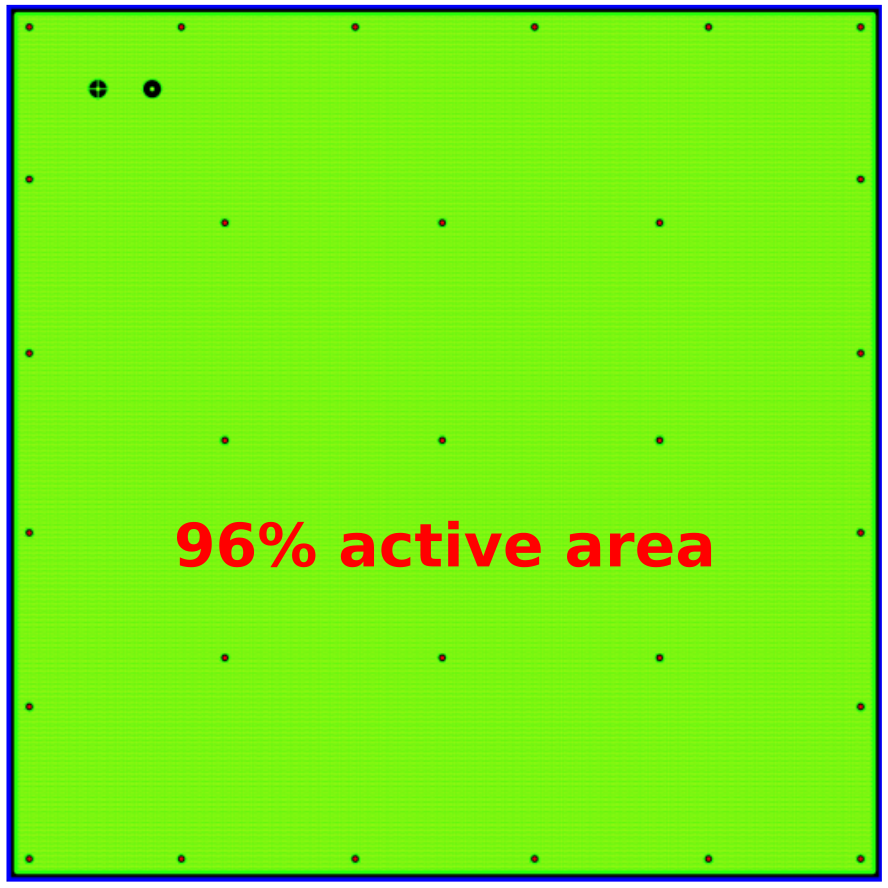
\includegraphics[width=\textwidth,keepaspectratio]{CFR-34.png}
                    \caption[Modèle de \gls{lem} CFR-34.]{Modèle de \gls{lem} CFR-34 utilisé dans le prototype 311. Les zones dépourvues de trous d'amplifications aux bords et autour des trous des vis et des connecteurs hautes tension sont plus petites que celles du modèle CFR-35.}
                    \label{fig::cfr34}
                \end{subfigure}
                \hfill
                \begin{subfigure}[t]{0.48\textwidth}
                    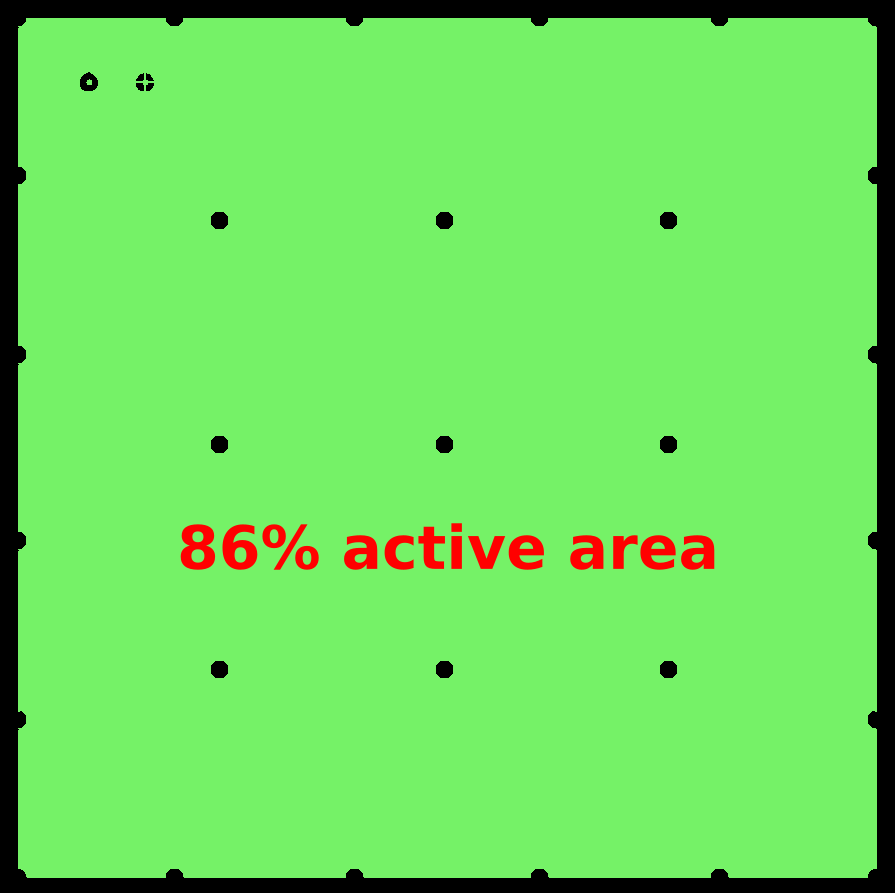
\includegraphics[width=\textwidth,keepaspectratio]{CFR-35.png}
                    \caption[Modèle de \gls{lem} CFR-35.]{Modèle de \gls{lem} CFR-35 utilisé dans le démonstrateur 666. Les zones dépourvues de trous d'amplifications ont été agrandies par rapport au modèle CFR-34 qui montrait des difficultés à tenir des tensions de l'ordre de \SI{3}{\kilo\volt}.}
                    \label{fig::cfr35}
                \end{subfigure}
                \caption{Fichier Gerber des modèles de \gls{lem} CFR-34 et CFR-35.}
                \label{fig::cfrs}
            \end{figure}
            Les \glspl{lem} sont l'élément central d'une \gls{tpc} à double phase d'argon. Ce sont eux qui vont permettre l'amplification du signal dans la phase gazeuse. Produit de plusieurs dizaines d'années de recherche et développement, ils ont prouvé être mieux adaptés aux amplifications dans les gaz nobles que les techniques utilisant des chambres à fils (\cite{Buzulutskov2000,Breskin2008}). Ce sont des \glspl{pcb} constitués d'une plaque de résine résine époxy PANASONIC R-1566W (\gls{fr4}) recouverte de chaque côté par une fine couche de cuivre. Des trous sont percés à travers cette plaque, au travers desquelles les électrons primaires, issues de l'interaction d'une particule avec l'argon liquide plus bas, sont accélérés par une forte différence de potentielle appliquée entre les deux couches de cuivre, créant un champ électrique de l'ordre de $\SI{35}{\kilo\volt\per\centi\meter}$. Ceci permet alors de déclencher une avalanche de Townsend (voir \autoref{sec::townsend_avalanche}) dont le résultat est un gain de plusieurs dizaines (\cite{Cantini2014}), et un très bon rapport signal sur bruit.
            
            Un effet à prendre en compte dans les détecteurs utilisant des amplificateurs comme les \gls{lem} est le chargement de ces derniers. En effet, les lignes de champs à travers les \gls{lem} sont tels que des électrons vont pouvoir terminer leur course sur le \gls{fr4} au lieu de traverser le dispositif. Une accumulation de ces électrons diminuera alors le champ d'amplification, entraînant une baisse de gain. Ce phénomène, étudié dans cet article \cite{Cantini2014}, peut être décrit par une décroissance exponentielle du gain à laquelle est associée un temps caractéristique (que l'on appellera temps de charge) qu'il convient de mesurer. Comme une exploitation des résultats n'a vraiment de sens qu'à gain constant, il est préférable de diminuer ce temps de charge afin d'atteindre au plus vite un régime permanent.
            
            Un autre problème potentielle est que des tensions trop importantes peuvent entraîner des décharges soudaines, entre la grille de un ou plusieurs \gls{lem}, au travers d'un ou plusieurs \gls{lem} ou entre un ou plusieurs \gls{lem} et les anodes. Ces décharges ont, par exemple, grandement limité la prise de données avec le prototype 311 qui n'a pas réussi à atteindre les tensions souhaitées en \autoref{sec::crp_intro}.
            
            Les \glspl{lem} de \gls{wa105} ont une surface de $50\times\SI{50}{\centi\meter\squared}$ permettant de couvrir les $\SI{36}{\meter\squared}$ du démonstrateur 666 avec 144 \glspl{lem}, et une épaisseur de $\SI{1}{\milli\meter}$. Ils sont percés de \numprint{400000} trous de $\SI{500}{\micro\meter}$ de diamètre, répartis selon un motif hexagonale sur la surface du \gls{lem} (voir \autoref{fig::LEM}). Chaque trou est entouré d'un anneau dépourvu de cuivre d'une épaisseur de $\SI{40}{\micro\meter}$ appelé rim, servant à assurer la stabilité en tension du \gls{lem} \cite{Breskin2008}. L'épaisseur de cuivre est de $\SI{40}{\micro\meter}$. Ils sont également percés de \numprint{29} trous de fixation au travers desquelles passent les entretoise et deux trous pour passer les connecteurs haute tension. Les spécifications précises sont décrites dans le \autoref{tab::lem_commun}.
            
            Les \glspl{lem} utilisés dans le prototype 311 ont un bord dépourvu de cuivre de $\SI{2}{\milli\meter}$, suivi d'un bord de $\SI{2}{\milli\meter}$ de cuivre dépourvu de trou. Des zones similaires sont présentes également autour des trous de fixation et des connecteurs haute tension. Les effets de ces zones sur la collection de charge et la résolution en énergie est présentée en \autoref{sec::zones_mortes}. Des tests de tenue en haute tension effectués à Saclay (voir \autoref{sec::test_HT}) sur les \glspl{lem} destinés au démonstrateur 666 ont permis de montrer que ce modèle (appelé CFR-34) ne permettait pas d'atteindre les tensions voulues, et un nouveau modèle (appelé CFR-35) a été proposé. Les bords ont été élargis, et sont constitués d'une zone de $\SI{1}{cm}$ dépourvue de cuivre suivi d'une zone de $\SI{5}{mm}$ de cuivre sans trous (voir \autoref{fig::cfrs}). C'est ce modèle qui a été gardé pour le démonstrateur 666. Les spécifications précises des deux modèles sont décrites dans le \autoref{tab::lem_diff}.
            
            Les choix des valeurs des différents paramètres communs aux deux modèles sont motivés par une étude réalisé par \gls{ethz} en 2014 \cite{Cantini2014}. Il y est montré qu'une épaisseur plus grande de \gls{fr4} correspond, comme attendu, à un gain plus grand, mais également à un temps de charge plus grand. Une largeur du rim plus grande correspond à un temps de charge plus grand, mais permet d'atteindre des gain plus grand \cite{Breskin2008}. Une disposition hexagonale des trous permet d'atteindre des gains plus grand qu'une disposition en carrés. Un diamètre des trous plus grand permet une meilleure stabilité en tension du \gls{lem} durant une exploitation de plusieurs jours, mais implique une baisse plus importante du gain après chargement du \gls{lem}.
            
            \begin{table}
                \centering
                \begin{tabular}{|l|c|c|}
                    \hline
                     & valeur & tolérance \\
                    \hline
                    Épaisseur d'époxy & \SI{1}{\milli\meter} & \\
                    Épaisseur de cuivre & \SI{60}{\micro\meter} & \\
                    Couche de finition & \SI{5}{\micro\meter} Ni$+\SI{0.1}{\micro\meter}$ Au & \\
                    Épaisseur totale & \SI{1.065}{\milli\meter} &  $-60/+\SI{20}{\micro\meter}$ \\
                    \begin{tabular}{@{}l@{}}Uniformité de \\ l'épaisseur\end{tabular} & $\pm \SI{40}{\micro\meter}$ & \\
                    Largeur du rim & \SI{40}{\micro\meter} & $\pm\SI{4}{\micro\meter}$ \\
                    Surface totale &  $499.5\times\SI{499.5}{\milli\meter\squared}$ & $+0/-\SI{0.2}{\milli\meter}$ \\
                    Nombre de trous & $\sim400000$ & \\
                    Diamètre des trous & $\SI{0.5}{\milli\meter}$ & $-0/+\SI{10}{\micro\meter}$ \\
                    \begin{tabular}{@{}l@{}}Distance centre à \\ centre entre \\ deux trous\end{tabular}  & $\SI{0.8}{\milli\meter}$ & \\
                    \hline
                \end{tabular}
                \caption{Caractéristiques des \gls{lem} communes aux deux modèles utilisés dans \gls{wa105}.\label{tab::lem_commun}}
            \end{table}
            
            \begin{table}
                \centering
                \begin{tabular}{|l|c|c|}
                    \hline
                     & CFR-34 & CFR-35\\
                    \hline
                    Bord -- zone sans cuivre & \SI{2}{\milli\meter} & \SI{10}{\milli\meter}\\
                    Bord -- zone avec cuivre sans trous & \SI{2}{\milli\meter} & \SI{5}{\milli\meter}\\
                    Trous de vis -- diamètre sans cuivre & \SI{4.2}{\milli\meter} & \SI{10}{\milli\meter} \\
                    Trous de vis -- anneau sans trous &  \SI{1.1}{\milli\meter} & \SI{5}{\milli\meter} \\
                    Trous de connecteur -- diamètre sans cuivre & \SI{10}{\milli\meter} & \SI{10}{\milli\meter} \\
                    Trous de connecteur -- anneau sans trous & \SI{1}{\milli\meter} & \SI{5}{\milli\meter} \\
                    \hline
                \end{tabular}
                \caption{Caractéristiques spécifiques aux modèles de \gls{lem} utilisés dans \gls{wa105}.\label{tab::lem_diff}}
            \end{table}
            
        
    \section{Les zones mortes des LEM}\label{sec::zones_mortes}
    
        Deux modèles de \glspl{lem} sont utilisés dans \gls{wa105}, chacun présentant des aires dépourvues de trous d'amplification pouvant constituer des zones mortes. Les effets de ces zones mortes sur la charge collectée et sur la résolution de la l'énergie détectée ont été simulés pour le modèle CFR-34 (utilisé dans le prototype 311). Une première sous-section traite de la méthode de simulation, sont ensuite présentés la carte d'efficacité ainsi créée et l'impact simulé sur la résolution en énergie. Une dernière sous-section discute des limites de cette simulation.
        
        \subsection{Méthode de simulation}
        
            \subsubsection{Carte de champ avec ANSYS}
                
                \begin{figure}[htbp]
                    \begin{subfigure}[t]{0.61\textwidth}
                        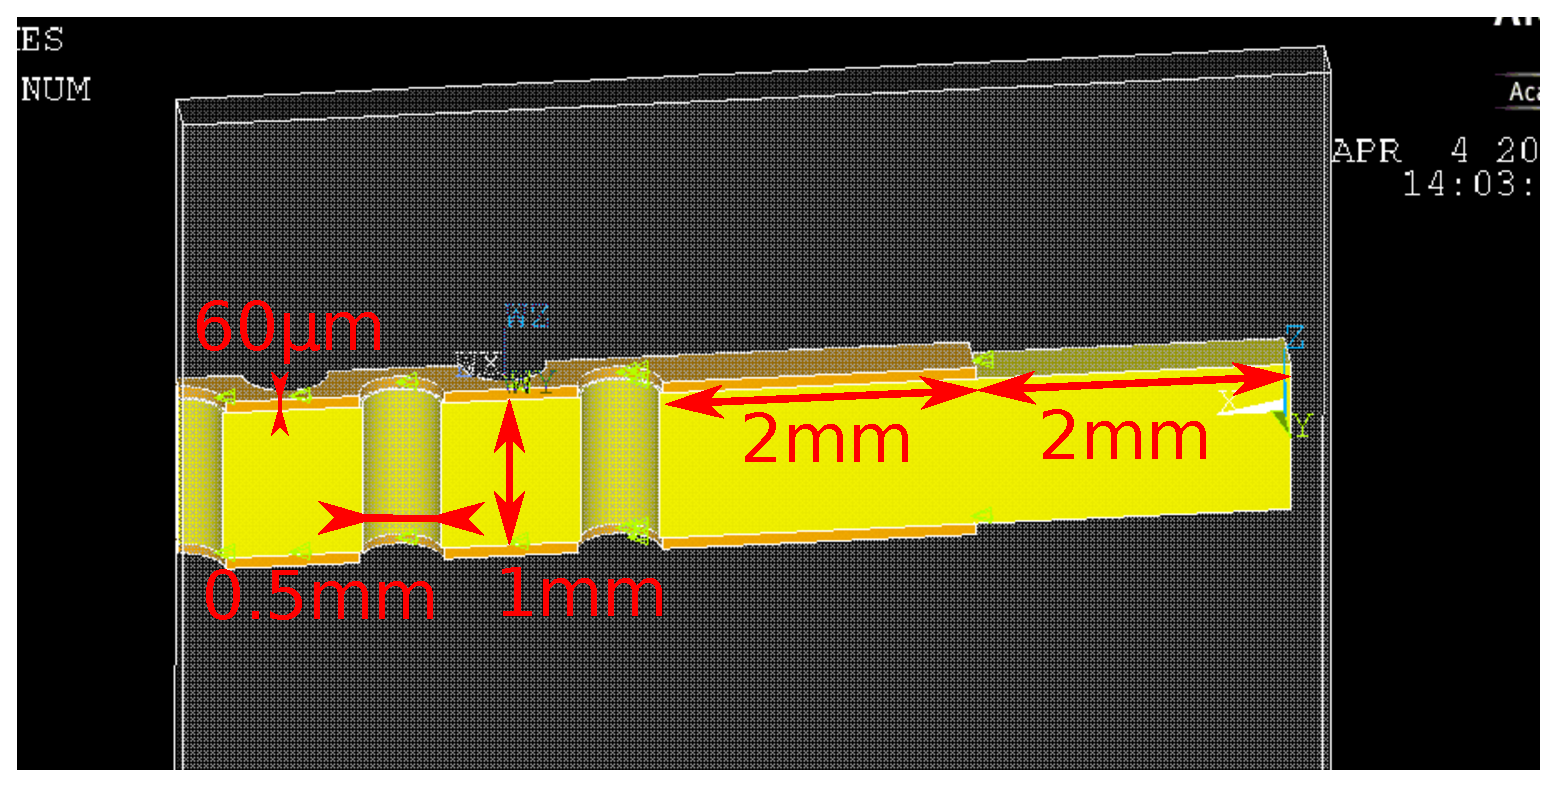
\includegraphics[width=\textwidth,keepaspectratio]{border_annotations.eps}
                        \caption[Bord d'un \gls{lem} modélisé avec \gls{ansys}.]{Bord d'un \gls{lem} modélisé avec \gls{ansys}.}
                        \label{fig::lem_border}
                    \end{subfigure}
                    \hfill
                    \begin{subfigure}[t]{0.31\textwidth}
                        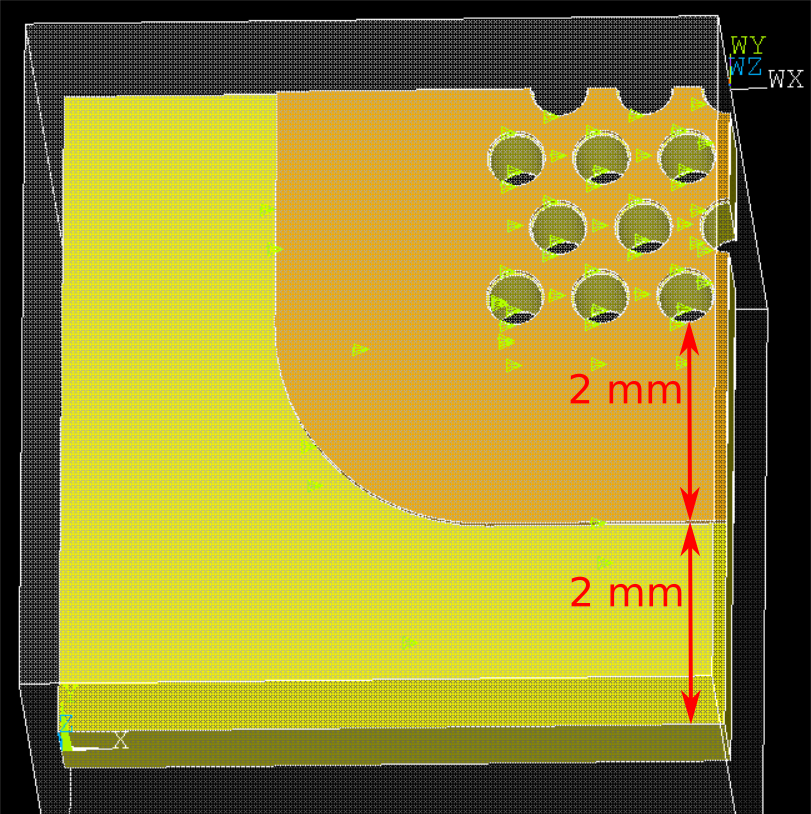
\includegraphics[width=\textwidth,keepaspectratio]{corner_annotations.png}
                        \caption[Coin d'un \gls{lem} modélisé avec \gls{ansys}.]{Coin d'un \gls{lem} modélisé avec \gls{ansys}.}
                        \label{fig::corner}
                    \end{subfigure}\\
                    \begin{subfigure}[b]{0.42\textwidth}
                        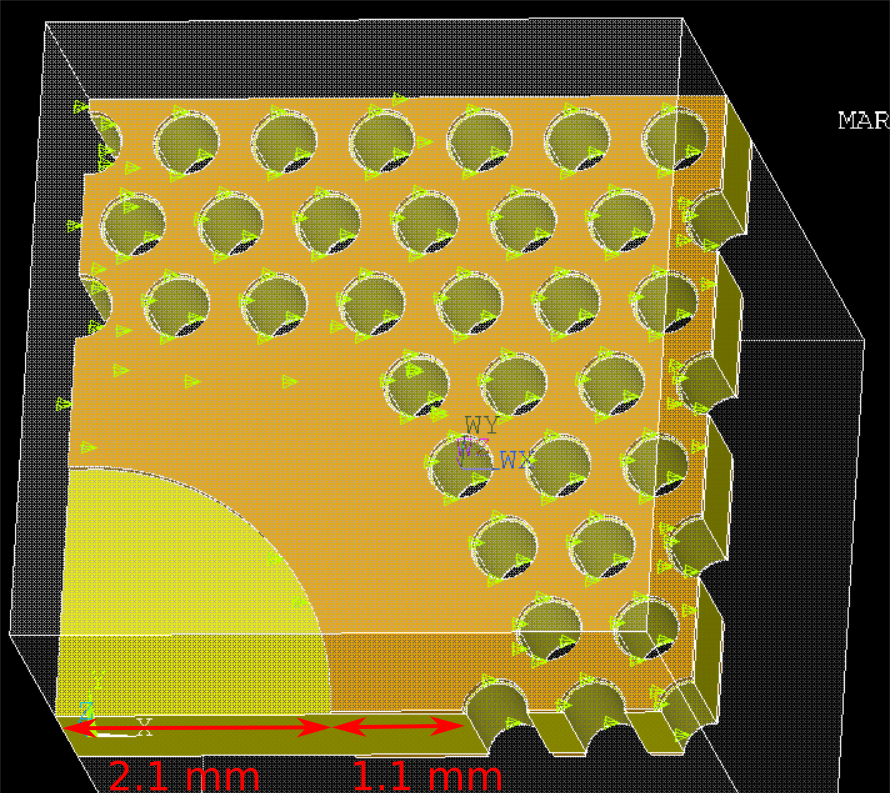
\includegraphics[width=\textwidth,keepaspectratio]{screw_annotations.png}
                        \caption[Zone autour d'un trou de vis d'un \gls{lem} modélisé avec \gls{ansys}.]{Zone autour d'un trou de vis d'un \gls{lem} modélisé avec \gls{ansys}.}
                        \label{fig::screw}
                    \end{subfigure}
                    \hfill
                    \begin{subfigure}[b]{0.48\textwidth}
                        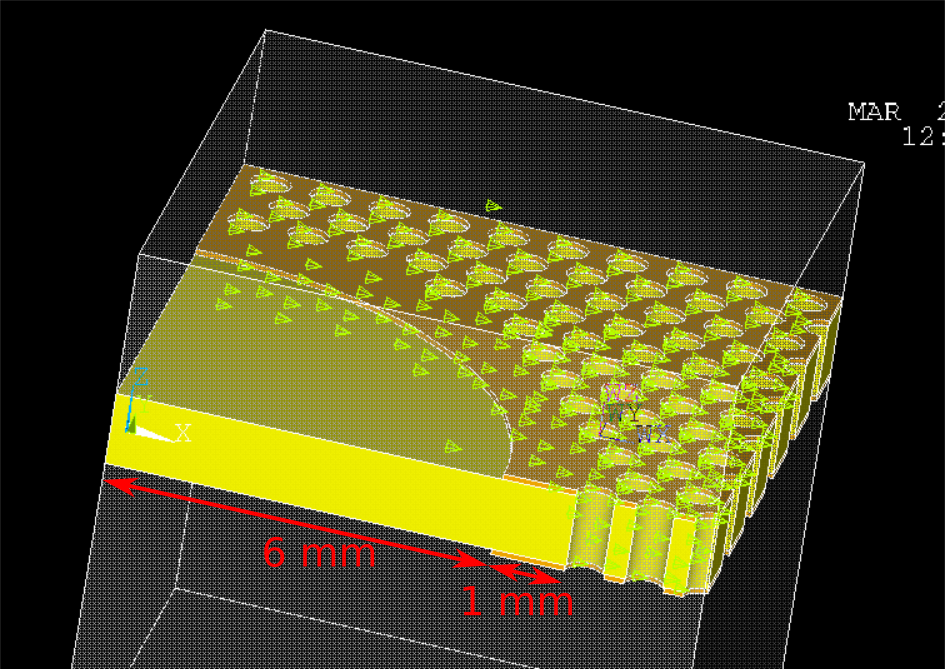
\includegraphics[width=\textwidth,keepaspectratio]{HT_annotations.png}
                        \caption[Zone autour d'un connecteur haute tension d'un \gls{lem} modélisé avec \gls{ansys}.]{Zone autour d'un connecteur haute tension d'un \gls{lem} modélisé avec \gls{ansys}.}
                        \label{fig::HT}
                    \end{subfigure}
                    \caption[Zones mortes d'un \gls{lem} modélisé avec \gls{ansys}.]{Zones mortes d'un \gls{lem} du modèle CFR-34 utilisé dans le prototype 311, modélisées avec \gls{ansys}. Les conditions de symétrie aux limites permettent de ne simuler qu'une "maille élémentaire" de chaque géométrie.}
                    \label{fig::zones_mortes}
                \end{figure}
            
                Le logiciel \gls{ansys}, utilisant la méthode des éléments finis, a été utilisé pour générer la carte du champ électrique à travers le \gls{crp} pour différentes zones : 
                \begin{itemize}
                    \item Les quatre bords des \glspl{lem}
                    \item Les quatre coins des \glspl{lem}
                    \item Les zones autour des vis de fixation
                    \item Les deux zones autour des connecteurs haute tension
                \end{itemize}
                Les bords du \gls{lem} présentent $\SI{2}{\milli\meter}$ de \gls{fr4} sans cuivre puis $\SI{2}{\milli\meter}$ de cuivre sans trous (\autoref{fig::lem_border}), idem pour les coins (\autoref{fig::corner}). Les zones autour des vis sont simplifiées en un cercle de \gls{fr4} plein, de rayon $\SI{2.1}{\milli\meter}$ entouré d'une zone de cuivre sans trous d'amplification formant un anneau de rayon extérieur $\SI{3.2}{\milli\meter}$ (\autoref{fig::screw}). Les zones autour des connecteurs haute tension ont été modélisées de la même manière, avec un cercle de \gls{fr4} plein de $\SI{5}{\milli\meter}$ et un anneau de cuivre sans trou d'amplification de rayon extérieur $\SI{6}{\milli\meter}$ (\autoref{fig::HT}). Des conditions de symétries sont appliquées au bord des modèles afin de n'avoir à simuler que les géométries présentées en \autoref{fig::zones_mortes}. 
                Les potentiels électriques utilisés pour cette simulation sont : 
                \begin{itemize}
                    \item $\SI{-1000}{\volt}$ entre l'anode et le haut du \gls{lem}, correspondant à un champ d'induction de $\SI{-5}{\kilo\volt}$
                    \item $\SI{-3500}{\volt}$ à travers le \gls{lem}, correspondant à un champ d'amplification de $\SI{-35}{\kilo\volt}$
                    \item $\SI{-2500}{\volt}$ entre le bas du \gls{lem} et la grille d'extraction, correspondant à un champ d'extraction de $\SI{-2.5}{\kilo\volt}$
                \end{itemize}
                
            \subsubsection{Transport des charges avec GarField}
            
                \begin{wrapfigure}[22]{r}{0.4\textwidth}
                    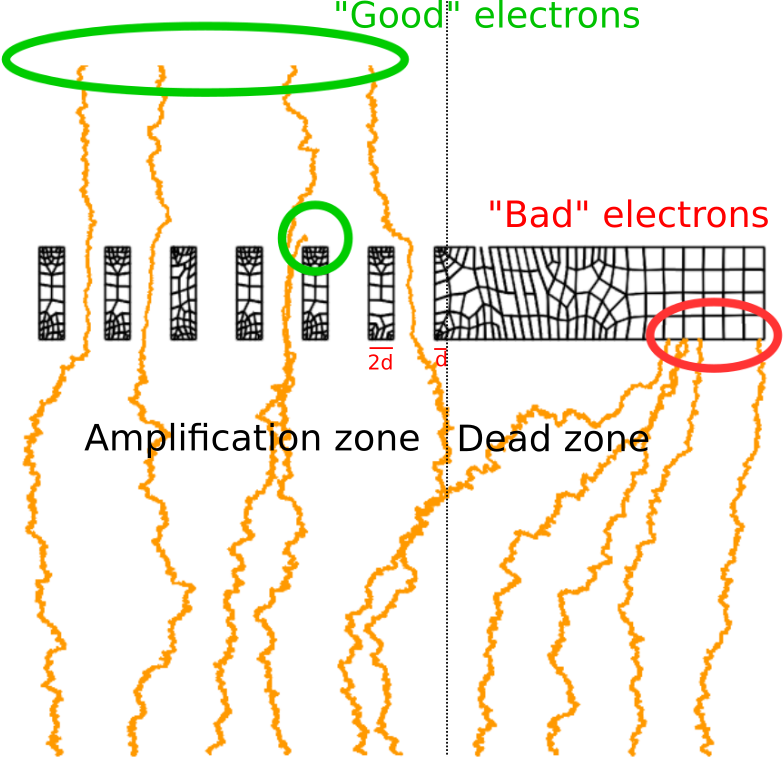
\includegraphics[width=0.4\textwidth,keepaspectratio]{drift_example.png}
                    \caption[Dérive de 10 électrons dans la carte de champ du bord d'un \gls{lem} avec Garfield.]{Dérive de 10 électrons dans un example 2D de carte de champ du bord d'un \gls{lem} créée avec \gls{ansys} par le logiciel Garfield. Le cercle rouge indique les électrons finissant leur dérive sur la zone morte, les cercles verts indiquent les électrons finissant leur dérive sur la zone d'amplification. La simulation d'avalanche n'est pas activée afin d'accélérer le calcul.}
                    \label{fig::drift_example}
                \end{wrapfigure}
                
                Afin d'estimer l'impact sur la dérive des électrons des zones décrites précédemment, le logiciel GarField \cite{garfield} a été utilisé pour simuler le parcours de \numprint{10000} électrons, générés selon une distribution plate, entre la zone de transition liquide--gaz et le \gls{lem}. Les électrons n'étaient pas générés dans le liquide afin de s'affranchir de l'efficacité d'extraction liquide--gaz décrite en \autoref{sec::efficacites}, mais un demi-millimètre au dessus, avec une énergie initiale nulle. La \autoref{fig::drift_example} %talk CERN
                montre le résultat pour une simulation de 10 électrons (l'avalanche est désactivée dans cette étude) : 5  atteignent la zone d'amplification tandis que 5 autres sont déviés sur le bords du \gls{lem}.
                
        \subsection{Résultat : carte d'efficacité}
        
            Un électron est considéré comme "bon" si il atteint la zone d'amplification, qu'il passe ensuite à travers un trou ou non. La \autoref{fig::drift_example} montre la limite de cette zone. Pour chaque électron, la position initiale est enregistrée, ainsi que le fait qu'il ait atteint ou non la zone d'amplification. Sont alors calculées la distribution de toutes les positions initiales des électrons et la distribution des positions initiales des électrons atteignant la zone d'amplification. Le ratio de la seconds distribution sur la première défini l'efficacité de transmission en fonction de la position. Le résultat pour les quatre zones mortes est montré en \autoref{fig::histo_eff}.
            
            \begin{figure}[htbp]
                \begin{subfigure}[t]{0.48\textwidth}
                    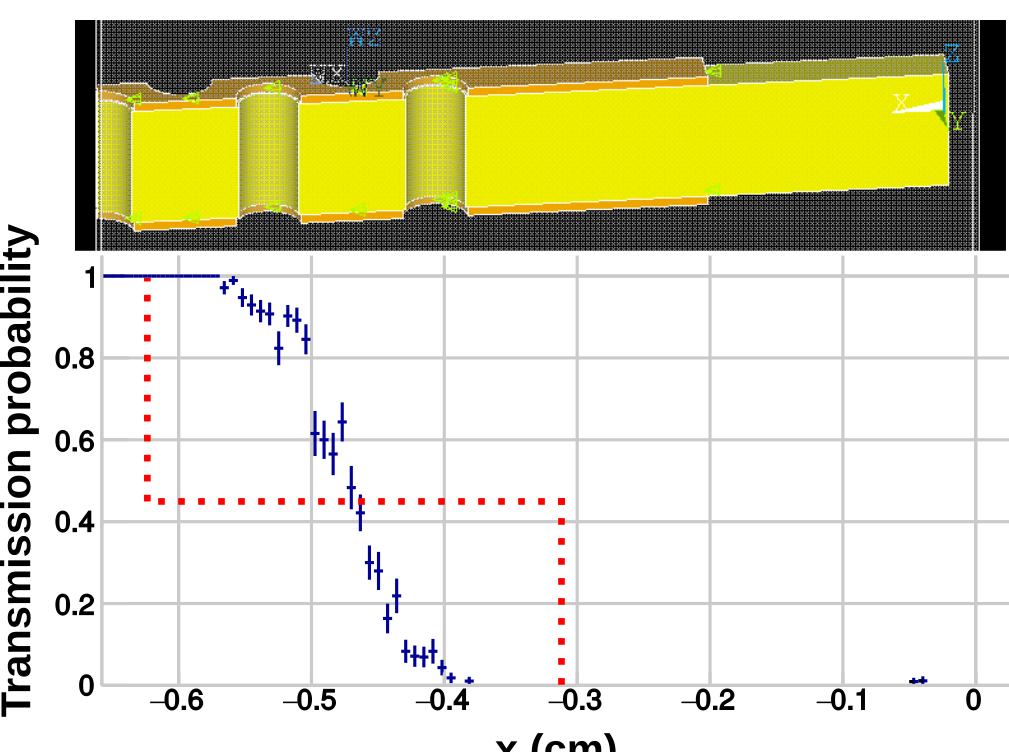
\includegraphics[width=\textwidth,keepaspectratio]{histo_bar.png}
                    \caption{Probabilité de transmission d'un électron en fonction de sa position initiale sous le bord d'un \gls{lem}. Les lignes pointillées indiquent les positions des deux premiers canaux de lecture de l'anode au dessus du bord.}
                \end{subfigure}
                \hfill
                \begin{subfigure}[t]{0.48\textwidth}
                    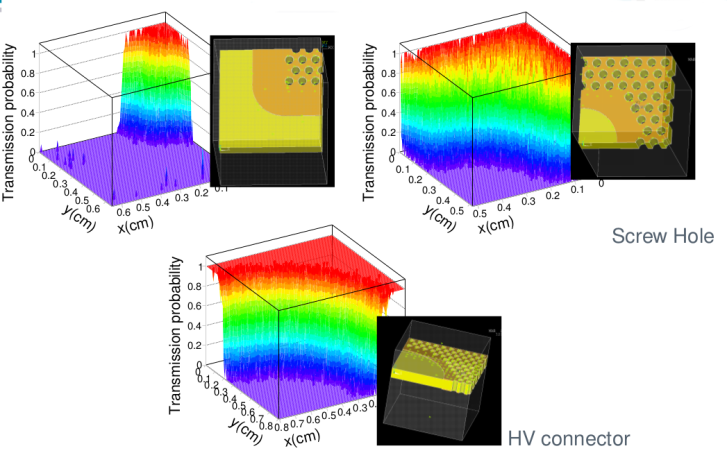
\includegraphics[width=\textwidth,keepaspectratio]{histo_corner_screw_hv.png}
                    \caption{Probabilité de transmission d'un électron en fonction de sa position initiale sous le coin, un trou de vis et un connecteur haute tension d'un \gls{lem}.}
                \end{subfigure}
                \caption[Probabilité de transmission des zones mortes d'un \gls{lem}.]{Probabilité de transmission d'un électron en fonction de sa position initiale après extraction sous les différentes zone mortes d'un \gls{lem} du modèle CFR-34.}
                \label{fig::histo_eff}
            \end{figure}
            
            En redéfinissant la taille des bins des histogrammes ainsi obtenus à la largeur des canaux de lecture des anode (\SI{0.3125}{\centi\meter}), il est possible de créer la carte d'efficacité complète montrée en \autoref{fig::eff_map}. Il apparaît alors que les pertes principales auront lieu sur les bords des anodes, où les premiers canaux ne devraient voir aucune charge tandis que les seconds canaux devraient voir moins de la moitié de la charge.
            
            \subsubsection{Comparaison aux données}
            
                %à faire
            
        \subsection{Résultat : impact sur la résolution}
            
            \begin{wrapfigure}{r}{0.4\textwidth}
                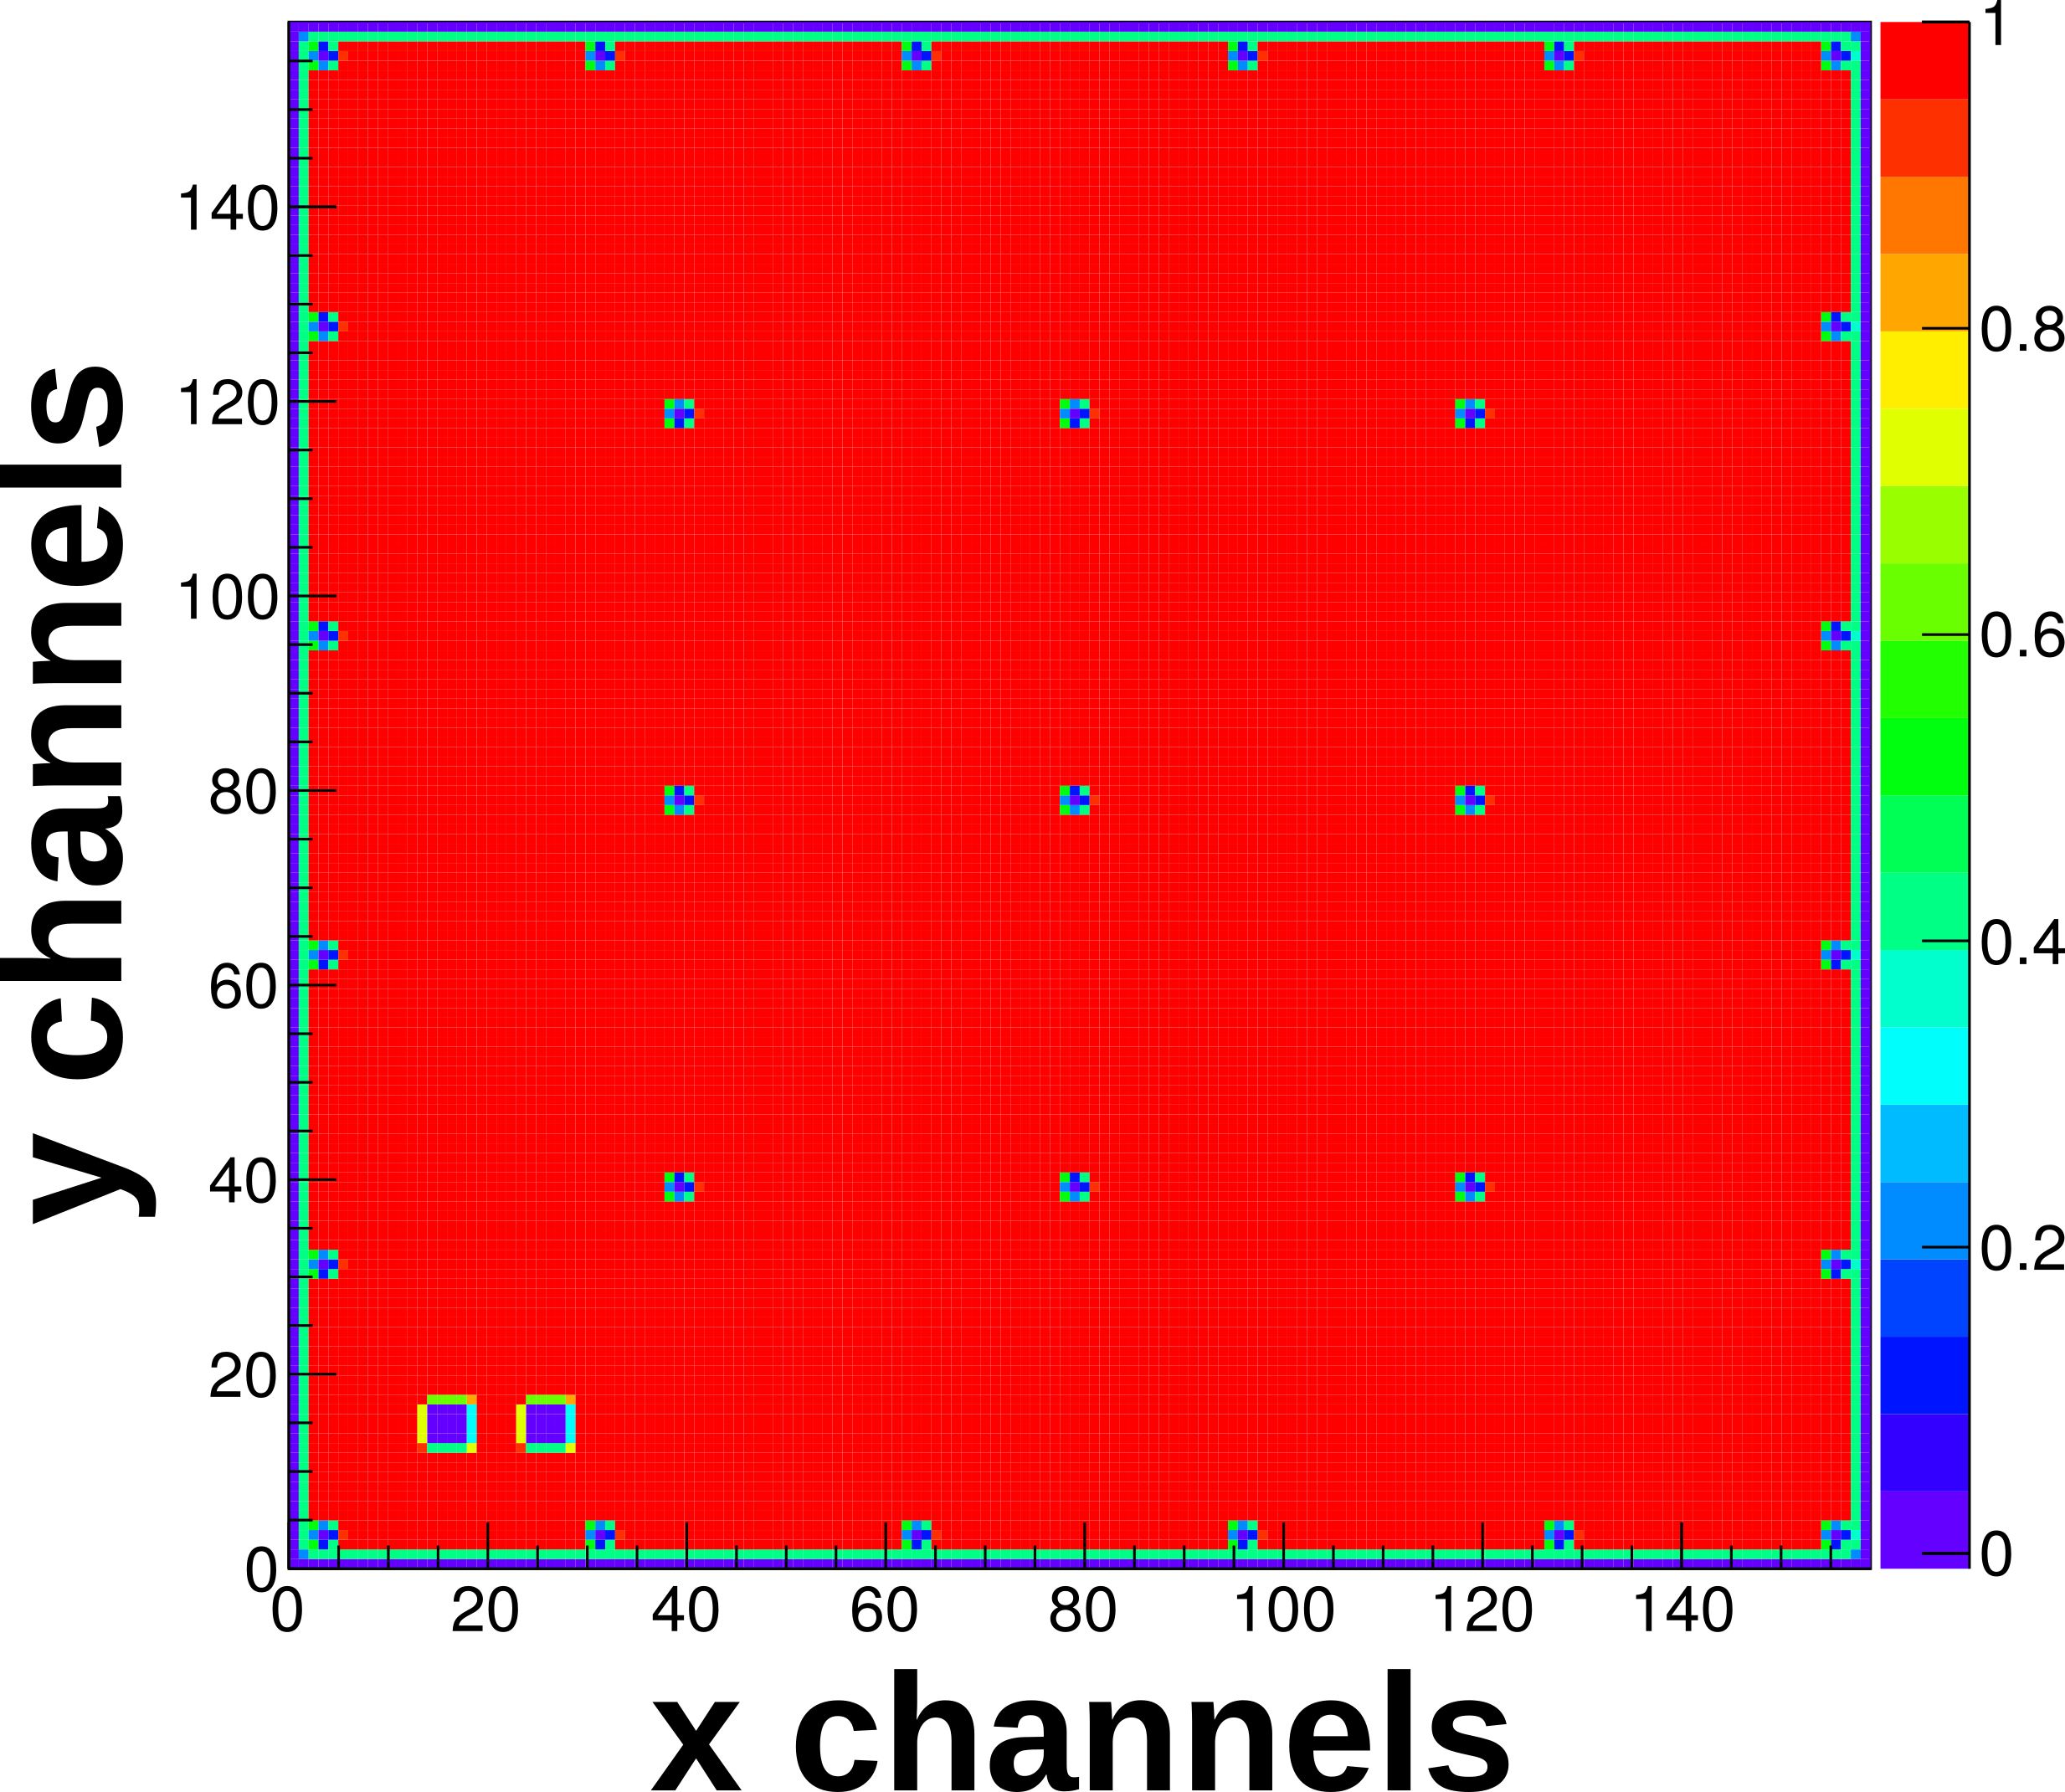
\includegraphics[width=0.4\textwidth,keepaspectratio]{eff_map.png}
                \caption[Carte d'efficacité d'un \gls{lem} du modèle CFR-34.]{Carte d'efficacité d'un \gls{lem} du modèle CFR-34. Les axes $x$ et $y$ représentent les \numprint{160} canaux des vues de l'anode se situant au dessus du \gls{lem}. La bar de couleur indique la fraction de charge qui atteindra chaque pixel ainsi formé.}
                \label{fig::eff_map}
            \end{wrapfigure}
        
            Cette étude a été faite avec le logiciel QScan, décrit en \autoref{sec::qscan}. La carte d'efficacité du \gls{lem} y a été implémentée, et plusieurs types de particules à plusieurs impulsions initiales ont été simulées dans le démonstrateur de 666\footnote{Ce travail a été fait en début de thèse. Nous ignorions à l'époque que le modèle des \glspl{lem} changerait pour le démonstrateur 666.}.
            
            J'ai regardé l'effet sur la charge totale arrivant à l'anode, avant reconstruction. Les effets de diffusion longitudinale et verticale sont simulés par des répartitions gaussiennes en temps et en espace de la charge (voir \cite{Agostino2014}).
            %cité dans Charge Collection
            %TODO ajouter plots
            
        
        \subsection{Limites de cette simulation}
        
            Cette simulation n'a été faite que pour une configuration du champ électrique à travers le \gls{crp}. Or des variations du champ d'extraction et/ou du champ d'amplification vont modifier les lignes de champs proches du \gls{lem}, il est donc probable que les probabilités de transmission en soient impactées. La méthode de simulation décrite plus haut peut tout à fait être répétée dans une étude future pour d'autre configurations du champ à travers le \gls{crp}.
            
            De plus, cette étude n'a été faite que pour le modèle CFR-34, qui n'est finalement pas utilisé dans le démonstrateur 666 et ne le sera pas non plus dans \gls{dune}.
            
            Le phénomène de charge du \gls{lem} au cours d'une opération longue d'une \gls{dlartpc} aura également un impact sur le champ électrique proche des zones mortes, où un grand nombre d'électrons est supposé s'accumuler. Cet effet n'est pas pris en compte par la méthode de simulation décrite ici.
        
    \section{Préparation, caractérisation et test à l'IRFU}
    
        Le \gls{cea} Saclay était en charge de la production de la moitié des \glspl{lem} et anodes du démonstrateur 666, l'autre moitié étant à la charge du \gls{cern}. Il était également en charge des tests haute tension et des contrôles métrologiques de tous les \glspl{lem} du démonstrateur 666. Un appel d'offre pour les modèle a été lancé en février 2017 et l'entreprise ELTOS a été retenue. Il a été demandé à l'entreprise d'effectuer plusieurs mesures sur les \glspl{lem} produits : l'épaisseur de la plaque d'époxy et des couches de cuivre, l'épaisseur des rims, la taille des trous d'amplification ainsi que les caractéristiques diélectriques. Le \gls{cea} a par la suite effectué des mesures complémentaires de l'épaisseur totale, ce paramètre ayant un impact particulièrement important sur le gain (voir \autoref{sec::townsend_avalanche}). Des tests de tenu en haute tension ainsi que des mesures de gain avec une source radioactive dans des conditions de pression de température équivalente à celle de la phase gazeuse d'une \gls{tpc} ont été réalisés dans une enceinte haute pression créée dans ce but. Enfin, des tests de continuité des pistes des anodes ont également été réalisés.
        
        \subsection{Production et préparation des LEM}
        
            La réalisation d'un \gls{lem} par ELTOS se fait de la manière suivante : perçage des plaques d'époxy déjà couvertes de cuivre avec changement fréquent des foret, nettoyage des résidus d'époxy et de métal dans les trous, polissage pour arrondir les bords des trous, gravure chimique des rims, traitement de surface nickel/or, détourage du \gls{lem} à ses dimensions finales et enfin nettoyage rinçage et étuvage.
                
            Sont ensuite effectuées des mesures décrites en \autoref{sec::thickness_comparison_eltos} pour s'assurer de la conformité au cahier des charges.
            
            Entre juillet 2017 et septembre 2018, le \gls{cea} a reçu et testé les 78 \glspl{lem} destinés au démonstrateur 666. Une fois les \glspl{lem} arrivés à l'\gls{irfu}, ils sont inspectés visuellement et les imperfections sont relevées. Ils sont ensuite envoyés à la métrologie afin que leurs épaisseurs soient mesurées (voir \autoref{sec::epaisseur}).
            
            L'étape suivante est alors la soudure de connecteurs haute tension et le collage des entretoises en Macor, qui permettront d'assurer une distance entre le \gls{lem} et l'anode de \SI{2}{\milli\meter}.
            
            \SI{24}{\hour} après le collage, les \glspl{lem} sont nettoyés pendant \numprint{3} minutes dans un bain ultrason d'eau désionisée et de lessive, à \SI{65}{\celsius} puis rincés d'abord à l'eau claire puis au Karcher avec de l'eau désionisée. Ils sont ensuite séchés une première fois avec à l'azote sous pression avant d'être séchés une seconde fois au four à \SI{80}{\celsius} pendant \numprint{3} heures. Ils sont ensuite polymérisés au four à \SI{160}{\celsius} pendant \numprint{3} heures.
        
        \subsection{Les mesures d’épaisseur des LEM}\label{sec::epaisseur}
        
            \subsubsection{Motivation : impact sur le gain}
            
                \begin{figure}[htbp]
                    \begin{subfigure}[t]{0.48\textwidth}
                        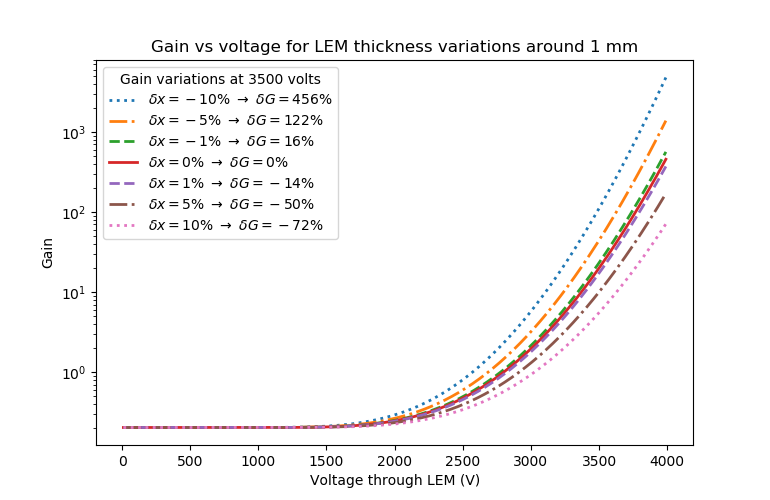
\includegraphics[width=\textwidth,keepaspectratio]{thickness_influence_on_gain.png}
                        \caption{Influence de l'épaisseur d'un \gls{lem} sur le gain.}
                    \end{subfigure}
                    \hfill
                    \begin{subfigure}[t]{0.48\textwidth}
                        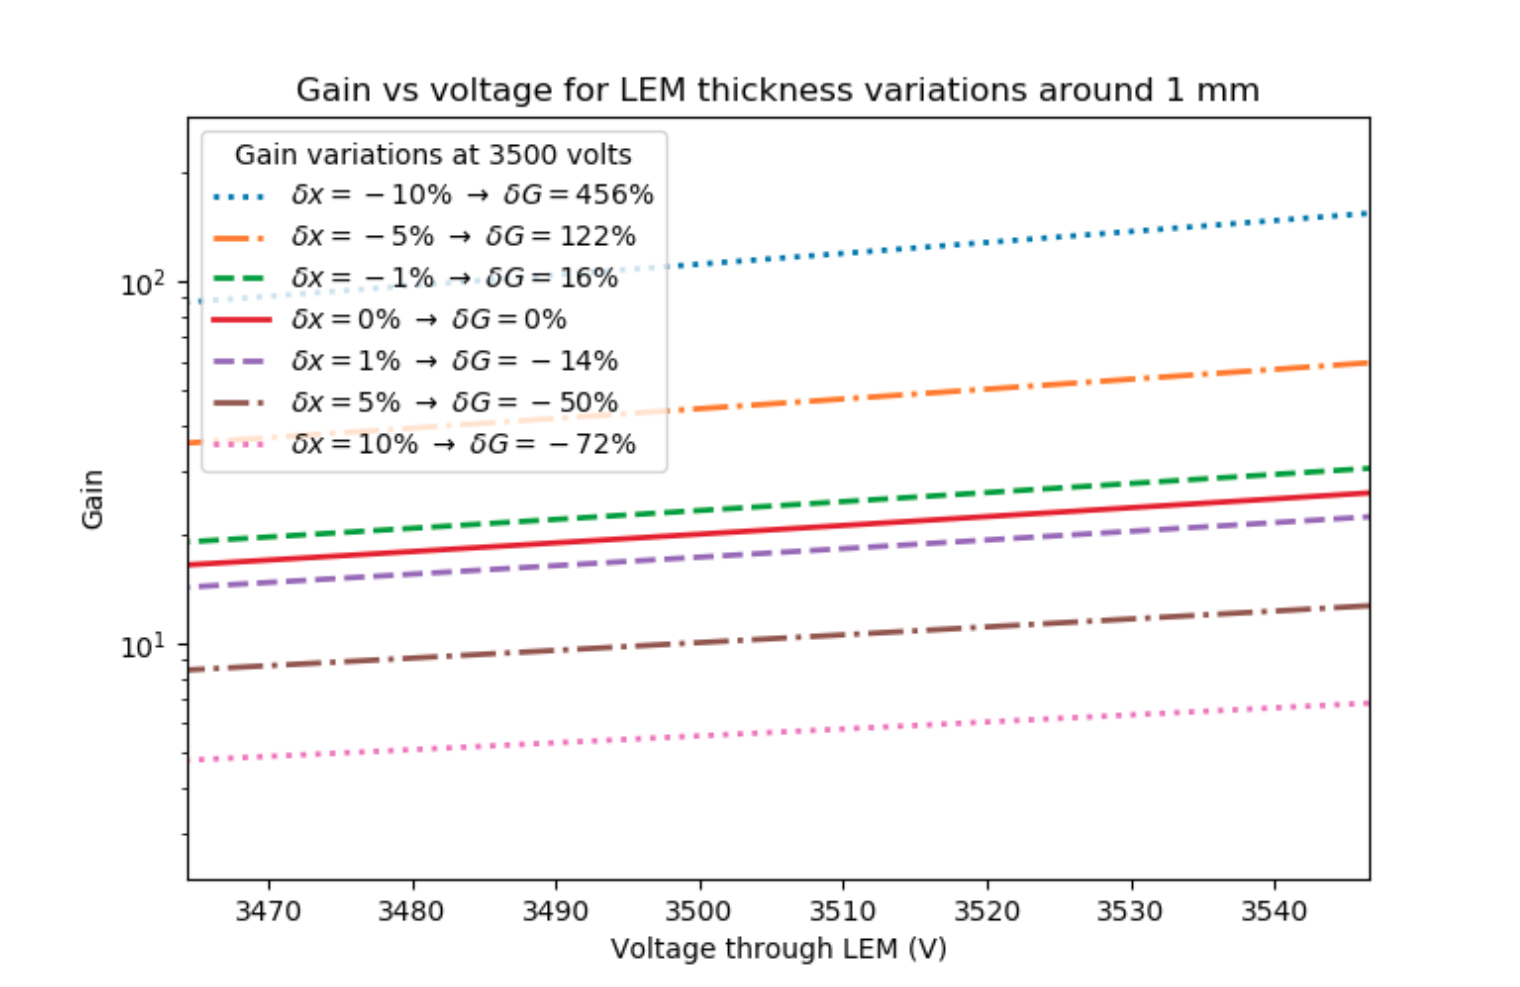
\includegraphics[width=\textwidth,keepaspectratio]{thicknes_influence_on_gain_zoom_35kV.png}
                        \caption{Influence de l'épaisseur d'un \gls{lem} sur le gain, agrandissement autour de \SI{35}{\kilo\volt\per\centi\meter}.}
                    \end{subfigure}
                    \caption[Influence de l'épaisseur d'un \gls{lem} sur le gain.]{Influence attendue de l'épaisseur d'un \gls{lem} sur le gain, d'après le formule \eqref{eq::townsend_avalanche_2} ajustée aux données présentées dans \cite{Cantini2014}. La référence d'épaisseur pour calculer les pourcentages est \SI{1}{\milli\meter}.}
                    \label{fig::thickness_influence_on_gain}
                \end{figure}
            
                La formule du gain à travers un dispositif amplificateur est rappelée ici (voir \autoref{sec::townsend_avalanche} pour plus de détails) :
                \begin{equation}\label{eq::townsend_avalanche_2}
                    G = e^{A\rho d e^{-B\rho d/V}}
                \end{equation}
                Avec $\rho$ la densité de l'argon gazeux, $V$ le potentiel électrique entre les deux faces du \gls{lem}, $A$ et $B$ des constantes et $d$ la longueur de la zone d'amplification. Cette longueur $d$ correspond dans le cas d'un \gls{lem} à son épaisseur. Ce paramètre apparaît deux fois, dans la première et dans la seconde exponentielle, ses variations ont donc un impact significatif sur le gain (voir \autoref{fig::thickness_influence_on_gain}). Il est nécessaire de pouvoir quantifier ses variations pour les \glspl{lem} utilisés, nous avons donc mis en place un dispositif permettant de mesurer l'épaisseur des \glspl{lem} produits pour les deux \gls{crp} du $6\times6\times6$. Les résultats ainsi obtenus sont comparés aux résultats obtenus par ELTOS dans le \autoref{tab::comparaison_eltos}, ces dernières n'étant faites qu'aux bords des \gls{lem} et près des trous des vis.
                
            \subsubsection{Méthode expérimentale}
                %documentation dans hardware/lem_plaques/marbre_472
                \paragraph{Le marbre et le crayon optique}
                
                    \begin{wrapfigure}{r}{0.4\textwidth}
                        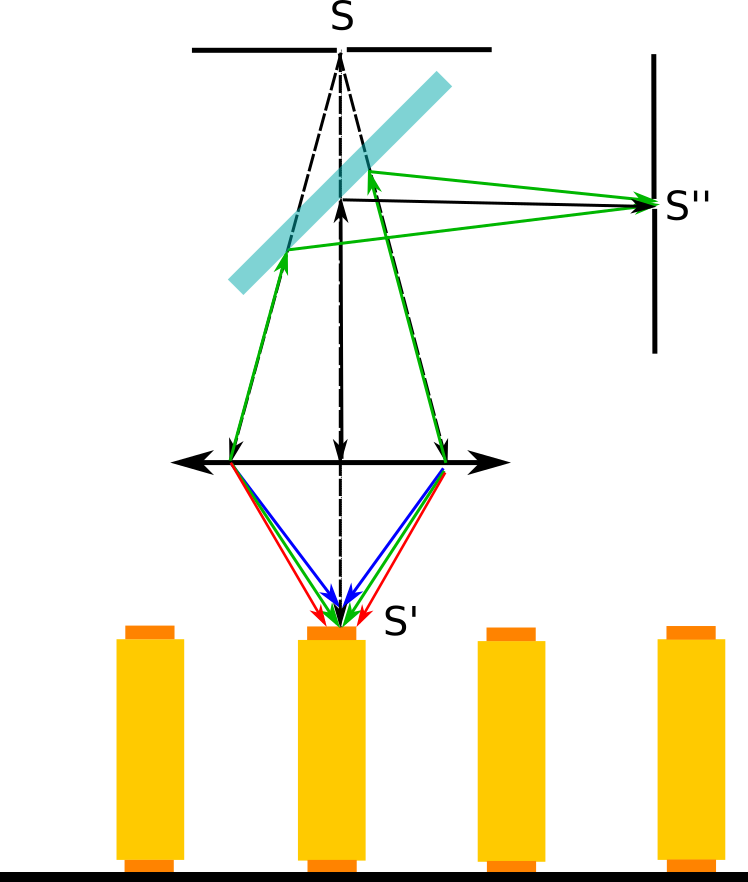
\includegraphics[width=0.4\textwidth,keepaspectratio]{CCI.png}
                        \caption[Schéma de la méthode de mesure \gls{cci}.]{Schéma de la méthode de mesure \gls{cci} servant à mesurer l'épaisseur des \gls{lem}. Les blocs oranges et jaunes représentent une vue en coupe, à l'échelle, d'un \gls{lem} posé sur le marbre avec ses trous d'amplification.}
                        \label{fig::CCI}
                    \end{wrapfigure}
                    
                    La technique d'\gls{cci} (voir \autoref{fig::CCI}), est employée pour mesurer l'épaisseur des \glspl{lem}. L'image $S'$ d'une source polychromatique ponctuelle $S$ est créée à la surface de l'objet à mesurer grâce à une lentille convergente. les rayons réfléchit en $S'$ retraversent la lentille et sont déviés grâce à un miroir vers un trou d'épingle $S''$, placé devant un spectromètre. Comme deux longueurs d'onde ne seront pas focalisées à la même distance de la lentille, seule un spectre très restreint de la lumière initiale atteindra le trou d'épingle. En faisant correspondre la longueur d'onde détectée à une distance à la lentille, il est ainsi possible de mesurer la distance entre la lentille et l'objet.% Le \autoref{tab::CCI} résume les caractéristiques du dispositif utilisé.
                    %plusieurs photo du dispositif
                    Pour que cette technique soit efficace, il faut disposer d'une surface plate la plus uniforme possible sur laquelle poser l'objet à mesurer. Dans notre cas, il s'agit d'un marbre micrométrique dont les variations de hauteur ont été mesurées autour de $\SI{5}{\micro\meter}$ (\autoref{fig::marbre}).
                    
                    La source polychromatique utilisée est un crayon optique munie d'une LED blanche donc l'intensité est ajustable manuellement. Ce crayon optique est monté sur un rail grâce à un chariot à coussin d'air, lui permettant de se déplacer sans frottement sur un axe $x$, dont la coordonnée est enregistrée au micron près.
                    
                    \begin{wrapfigure}{r}{0.4\textwidth}
                        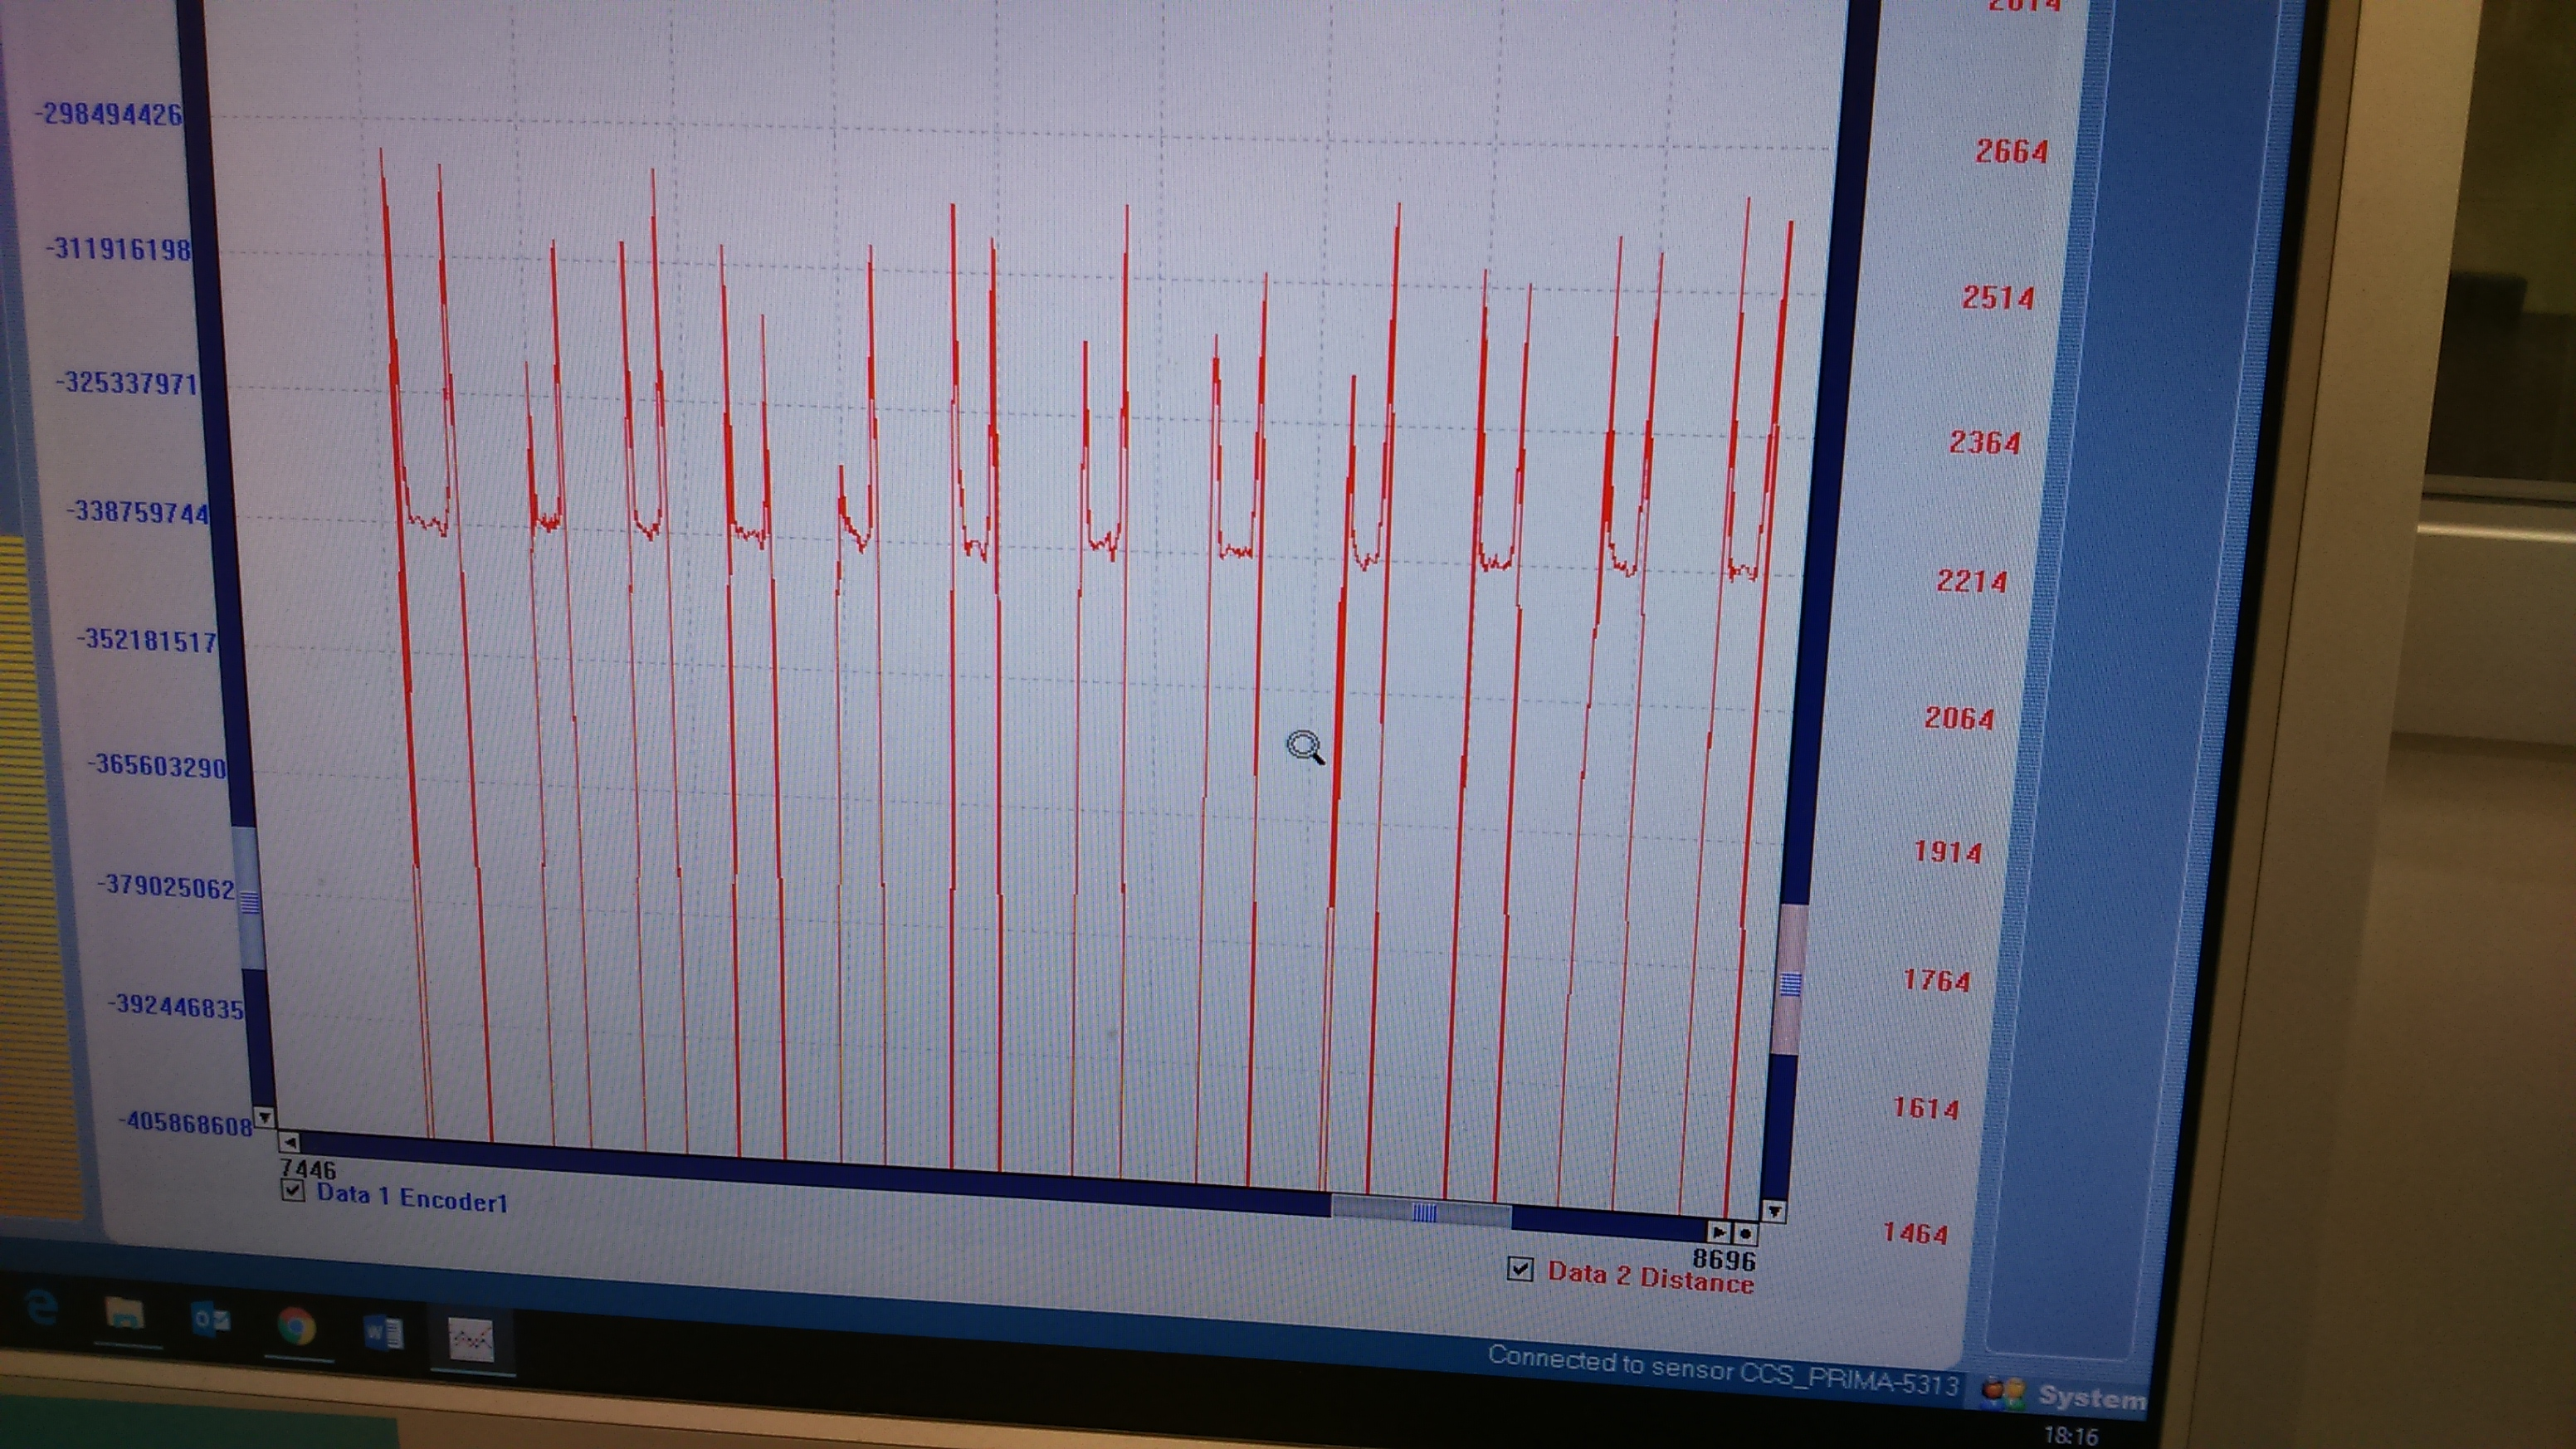
\includegraphics[width=0.4\textwidth,keepaspectratio]{soft_measure_LEM.JPG}
                        \caption[Représentation brute des données de mesure d'un \gls{lem} avec la technique \gls{cci}.]{Représentation brute des données de mesure d'un \gls{lem} avec la technique \gls{cci}. Les grands pics sont coupés à l'analyse.}
                        \label{fig::soft_measure_LEM}
                    \end{wrapfigure}
                    Le logiciel de mesure utilisé permet de visualiser en direct les variations de hauteurs au cours de la mesure. La forme des trous micrométriques des \gls{lem} est visible sur la \autoref{fig::soft_measure_LEM}, issue de ce logiciel. 
                    
                    A noter que due à l'absence de motorisation du chariot sur coussin d'air, ce dernier était poussé à la main, ce qui ne garantissait pas une vitesse constante.
                    
                \paragraph{Aplanir le LEM}
                    
                    %simplifier
                    Afin de mesurer l'épaisseur d'un \gls{lem} avec la technique CCI, il faut préalablement aplatir ce dernier. Ceci a été réalisée par une plaque en acier inox percée de 25 trous à travers lesquels les mesures étaient effectuée. 
                    
                    %La plaque en acier mesure $50\times50\times\SI{0.8}{\centi\meter}$ et est percée de 25 trous de $\SI{2}{\centi\meter}$ de diamètre à travers lesquels le crayons optique prend les mesures. Une épaisseur de PVC de $\SI{2.5}{mm}$ est ajoutée sous la plaque, pour une masse total de 16Kg.
                    %50*50*0.8 - (2*pi*0.8*25) * 8 /1000 = 15Kg d'acier
                    %50*50*0.25 - (2*pi*0.25*25) * 1.4 /1000 = 0.82 kG de PVC
                    
                    %Afin de ne pas abîmer la surface du \gls{lem} en posant la plaque dessus, une épaisseur de mousse de $50\times 50 \times \SI{0.5}{cm}$ est déposé sur le \gls{lem} avant d'y mettre la plaque. Cette feuille de mousse permet également d'homogénéiser la pression de la plaque à la surface du \gls{lem}.
                    
                    %La plaque et le \glspl{lem} sont positionnés sur le marbre à l'aide une équerre vissée au marbre (voir \autoref{fig::equerre}.)
                    
                    \begin{figure}[htpb]
                        \begin{subfigure}[t]{0.5\textwidth}
                            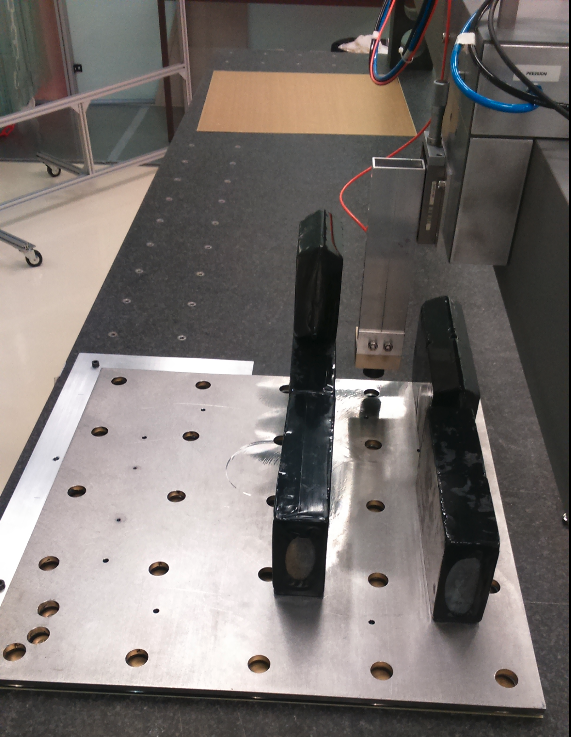
\includegraphics[width=\textwidth,keepaspectratio]{plate_and_bricks.png}
                            \caption[Système servant à aplanir le \gls{lem} sur le marbre.]{Système servant à aplanir le \gls{lem} sur le marbre. Le \gls{lem} est sous une plaque d'acier sur laquelle sont posées des briques de plomb le l'axe de mesure.}
                            \label{fig::plate_and_bricks}
                        \end{subfigure}
                        \hfill
                        \begin{subfigure}[t]{0.395\textwidth}
                            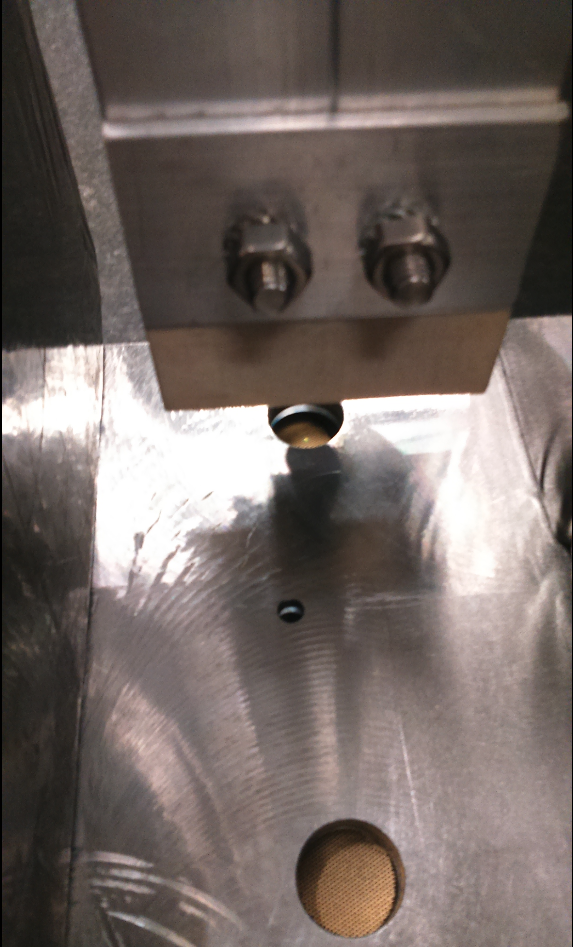
\includegraphics[width=\textwidth,keepaspectratio]{LEM_through_plate.png}
                            \caption[Vue du \gls{lem} mesuré à travers un trou de la plaque en acier.]{Vue du \gls{lem} mesuré à travers un trou de la plaque en acier. Le point vert correspond à la lumière du crayon optique.}
                            \label{fig::LEM_through_plate}
                        \end{subfigure}
                        \caption{Photographies du dispositif expérimental utilisé pour les mesures d'épaisseur.}
                        \label{fig::dispositif_experimental}
                    \end{figure}
                    Il a été observé que malgré la plaque, la distance indiquée par le \gls{cci} pouvait présenter des variations allant jusqu'à \SI{20}{\micro\meter} quand une plus grande pression était exercée sur le \gls{lem} proche de la mesure. Nous avons donc rajouté des briques en plomb de \SI{11}{\kilo\gram} disposées le long du chemin emprunté par le crayon optique (voir \autoref{fig::plate_and_bricks}). %Trois pièces d'aluminium pouvant être vissées au marbre ont été également rajoutées, permettant d'exercer une pression encore plus grande sur les bords bas, droit et gauche de la plaques.
                    
                    Malgré cela, le trou de mesure situé le plus au centre du \gls{lem} présentaient encore des variations de $10$ à $\SI{15}{\micro\meter}$. Il a donc était décidé d'ignorer ce trou de mesure.
                    
                    \begin{figure}[htpb]
                        \begin{minipage}{0.56\textwidth}
                           \begin{subfigure}[t]{\textwidth} 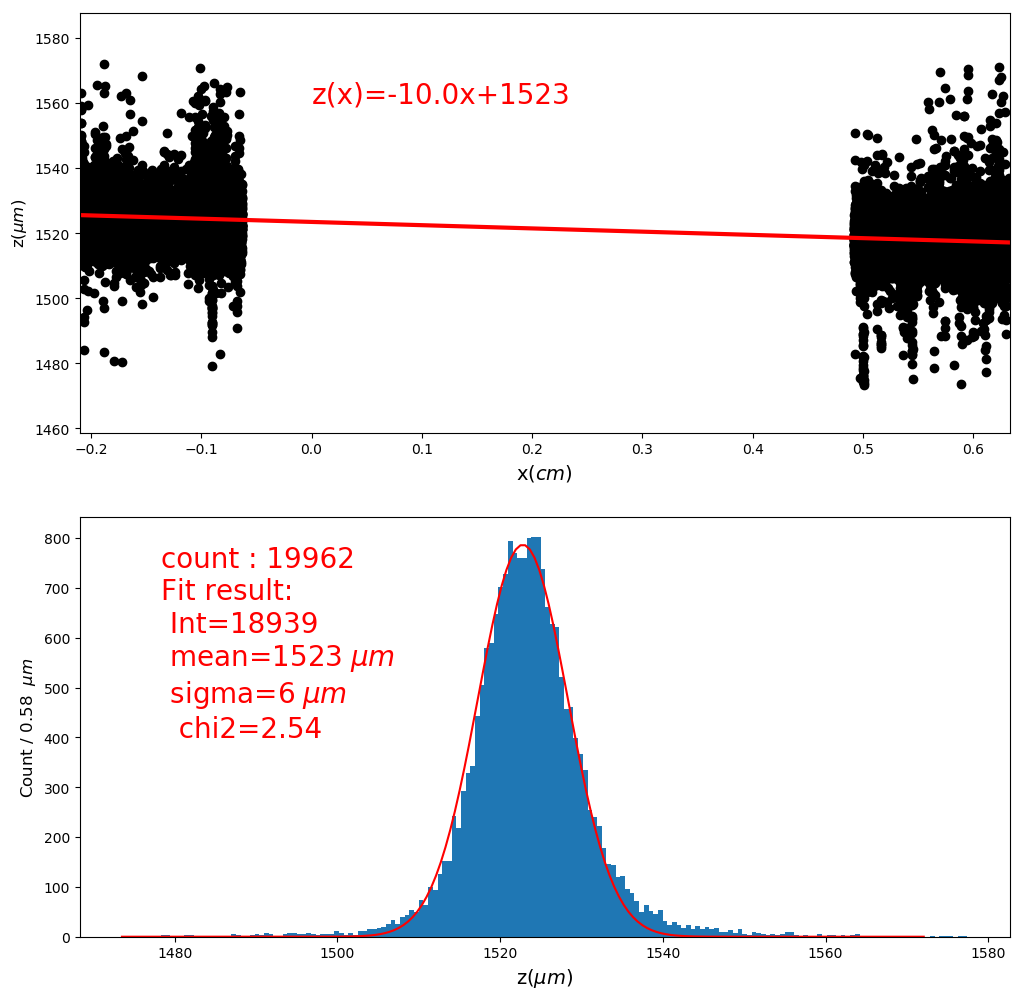
\includegraphics[width=\textwidth,keepaspectratio]{marbre.png}
                            \caption[Calibration du marbre.]{Calibration du marbre. Le graph du haut montre la pente du marbre le long de l'axe de mesure $x$, le graph du bas montre la dispersion de l'épaisseur du marbre après correction de la pente autour de $x=0$.}
                            \label{fig::marbre}
                            \end{subfigure}
                        \end{minipage}
                        \hfill
                        \begin{minipage}{0.38\textwidth}
                            \begin{subfigure}[t]{\textwidth}
                                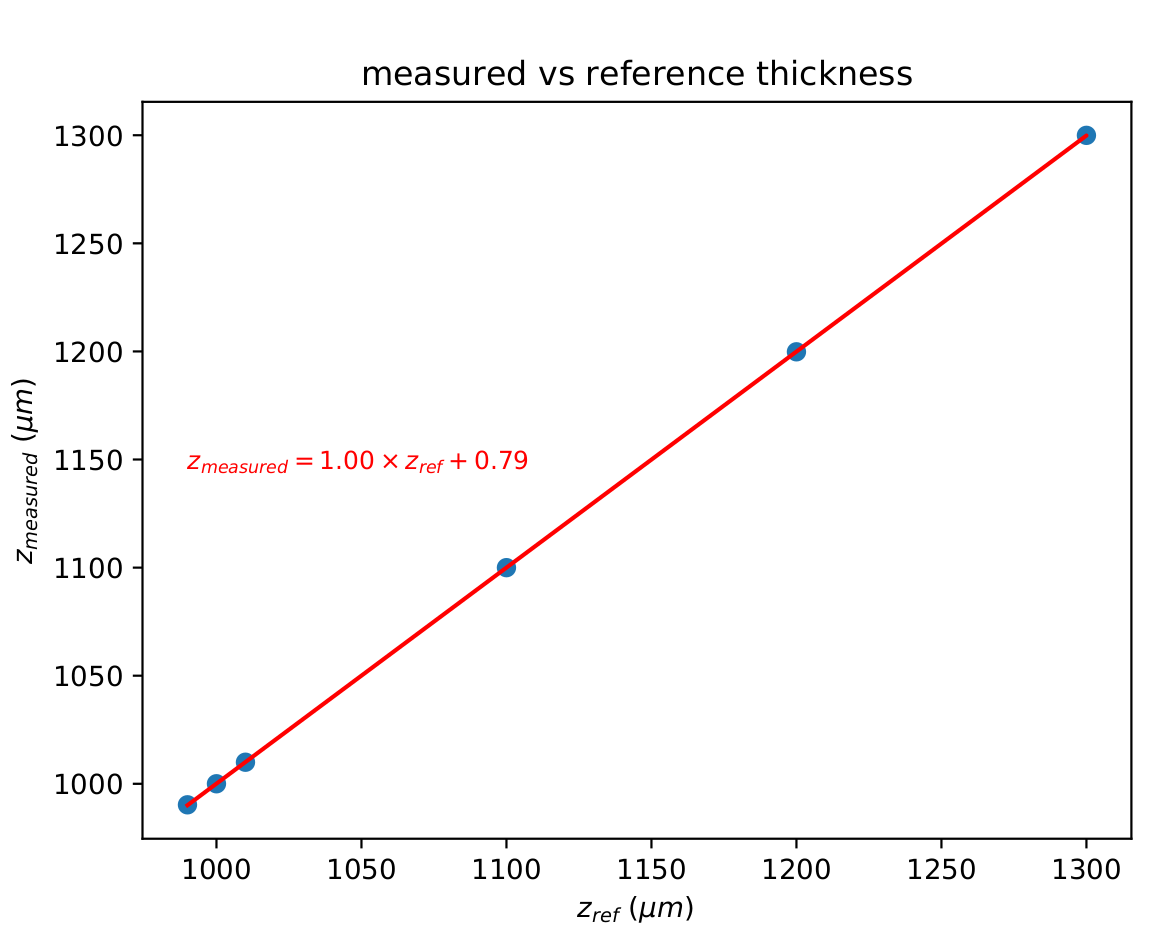
\includegraphics[width=\textwidth,keepaspectratio]{optic_response.png}
                                \caption[Calibration de la réponse du crayon optique.]{Calibration de la réponse du crayon optique avec six cales de différentes épaisseurs.}
                                \label{fig::optic_response}
                            \end{subfigure}
                            \begin{subfigure}[t]{\textwidth}
                                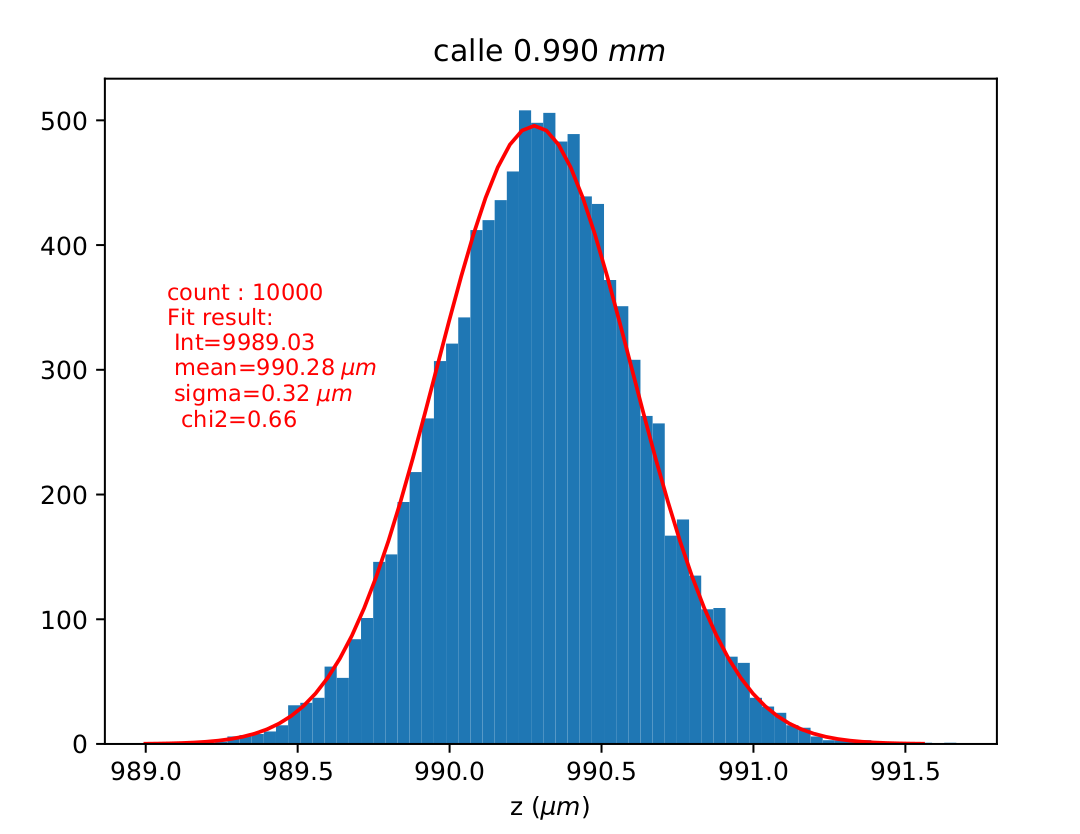
\includegraphics[width=\textwidth,keepaspectratio]{calle.png}
                                \caption[Dispersion de l'épaisseur mesurée d'une cale de \SI{0.99}{\milli\meter}.]{Dispersion de l'épaisseur mesurée d'une cale de \SI{0.99}{\milli\meter}.}
                                \label{fig::calle}
                            \end{subfigure}
                        \end{minipage}
                        \caption[Calibration du système de mesure \gls{cci}.]{Calibration du système de mesure \gls{cci}.}
                        \label{fig::calibration}
                    \end{figure}
                    Le mouvement selon l'axe $y$ ne peut se faire qu'en déplaçant manuellement la poutre, aussi les mesures ont été prises ligne par ligne.
                    
                    Due à la non mobilité en $y$ du dispositif de mesure, les mesures s'effectuaient ligne par ligne. Les mesures sont corrigées pour l'inclinaison du marbre, mesurée à chaque ligne. Celui-ci présentait une pente autour de $\SI{10}{\micro\meter\per\meter}$ (\autoref{fig::marbre}).
                    
                    La moyenne de la distribution des hauteurs du marbre corrigée pour la pente servait de zéro pour les mesures des épaisseurs du \gls{lem} lui même.
                    
                    La réponse du dispositif optique à la hauteur à mesurer a été vérifiée avec des cales d'épaisseur allant de $\SI{900}{\micro\meter}$ à $\SI{1300}{\micro\meter}$, en ajustant une droite d'équation $z_{mesure} = \alpha \cdot z_{cale} + \beta$ à la hauteur $z_{mesure}$ mesurée contre la hauteur $z_{cale}$ indiquée sur la cale. Le coefficient $\alpha$ est de $1.00$ et le coefficient $\beta$ de $\SI{0.72}{\micro\meter}$ (voir \autoref{fig::optic_response}).
                    
                    %Due à la non mobilité en $y$ du dispositif de mesure, les mesures s'effectuaient en ligne par groupe de cinq trous. D'abord, le marbre était mesuré à droite et à gauche du \gls{lem}, à une intensité de 100\%. Ensuite, la rangée de cinq trous était mesurée à une intensité de 30\%. La poutre sur laquelle repose le crayon optique était alors déplacée à la rangée suivante et la même opération était répétée. Les mesures du marbres à droite et à gauche servaient à déterminer la pente du marbre le long de l'axe $x$ ainsi que la distance à la lentille du bas du \gls{lem}, nécessaire pour calculer l'épaisseur de ce dernier.
                    
                    %Pour les deux rangées du haut, loin des pièces d'aluminium permettant un meilleur aplanissement, les briques en plomb était disposée le plus proche possible du trou de mesure, et nous vérifions à chaque fois que le niveau indiqué par l'appareil de mesure de bougeait pas de plus de $\SI{1}{\micro\meter}$ quand l'on exerçait un pression sur la plaque. Pour les trois autres rangées, les pièces d'aluminium étaient vissée soit du côté droit, soit du côté gauche, soit en bas suivant le trou mesuré. En effet, en serrant à droite, le côté gauche de la plaque d'acier pouvait se retrouver un peu soulevé, et inversement. Pour les trous centraux des troisième et quatrième rangées, les pièces en aluminium n'étaient pas serrées. Les briques en plomb étaient ajustées au mieux. Sur la plupart des \glspl{lem}, le trou central de la troisième rangée présenté une variation de plus de $\SI{10}{\micro\meter}$ quand une pression supplémentaire était exercée, aussi il a été décidé d'ignorer ce trou systématiquement.
                    
            \subsubsection{Résultats}
                    
                \begin{figure}[htpb]
                    \begin{subfigure}[t]{0.48\textwidth}
                        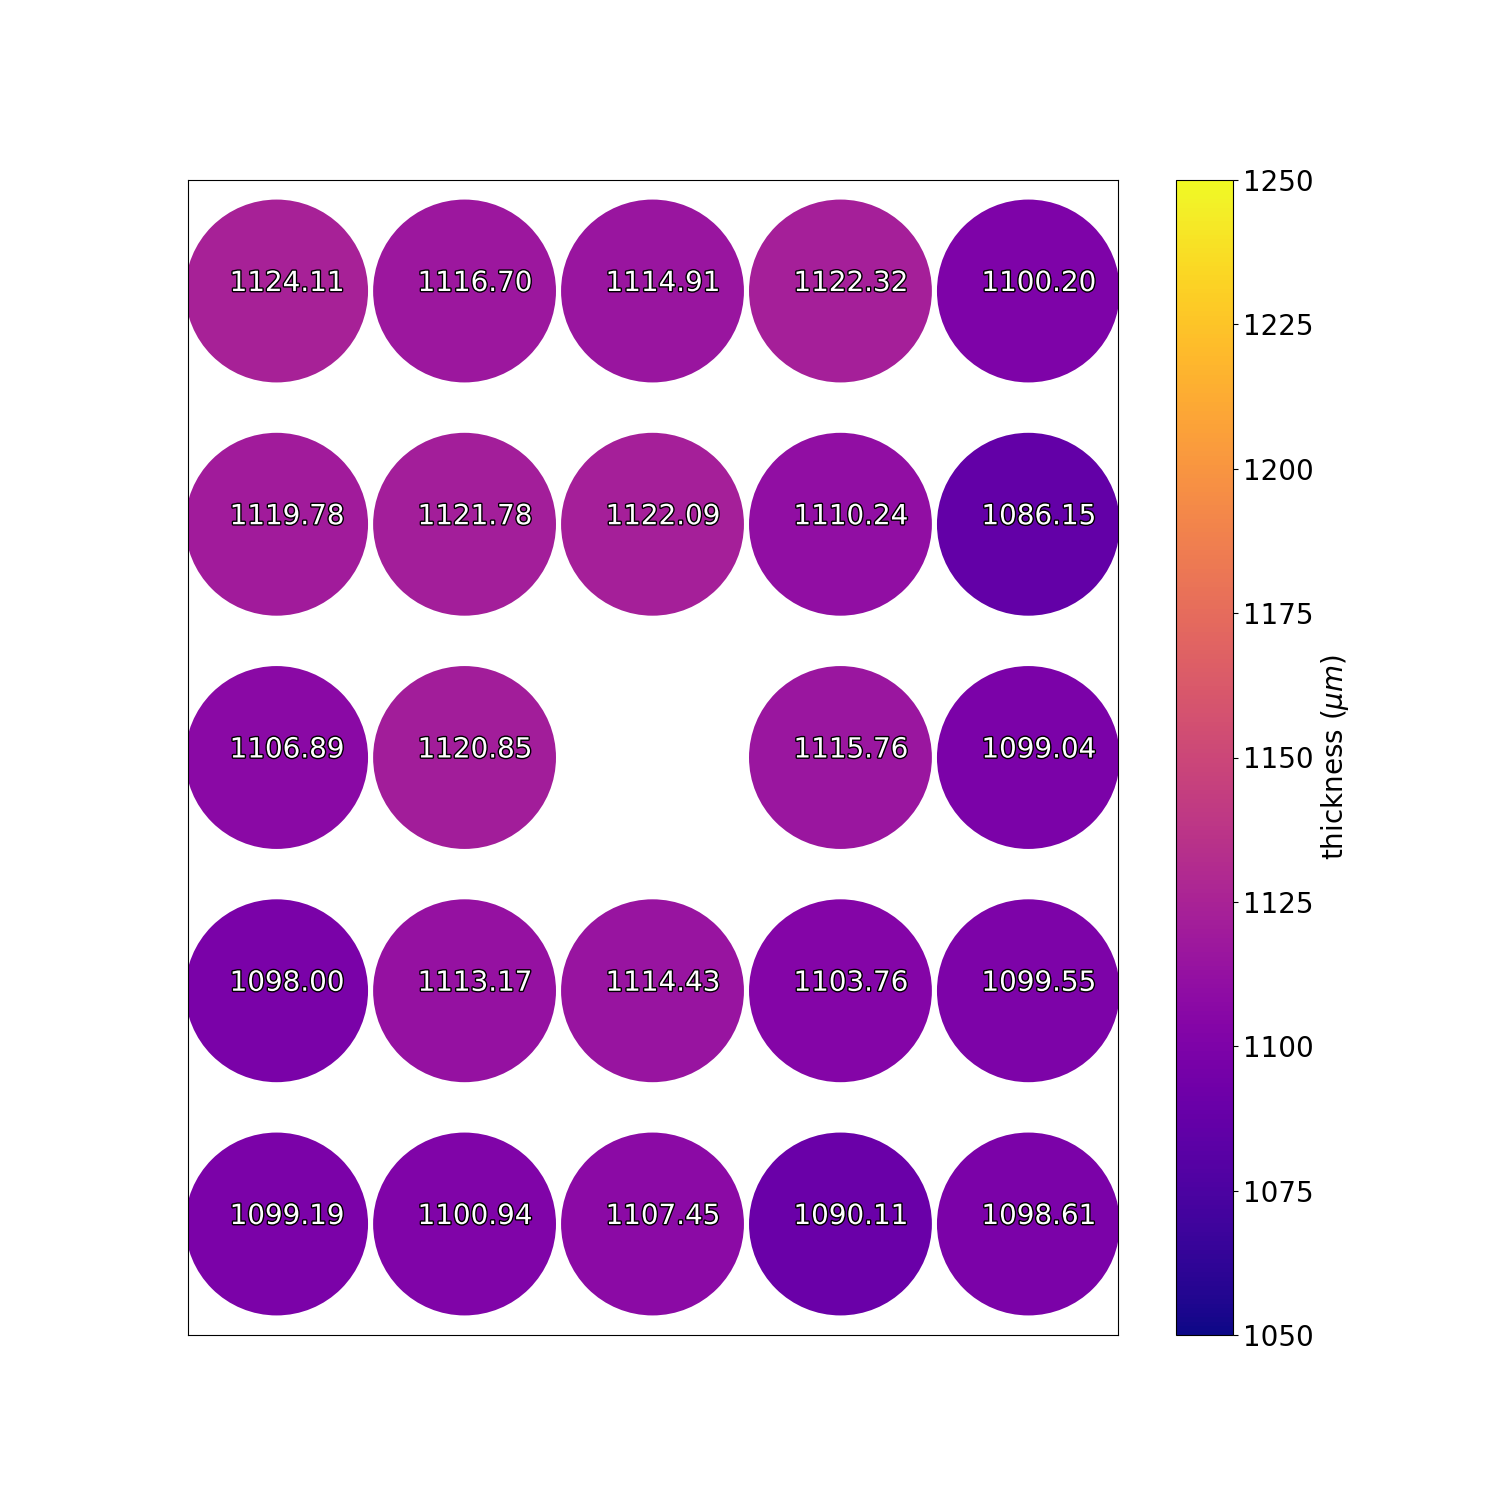
\includegraphics[width=\textwidth,keepaspectratio]{2D_LEM_thickness_distri.png}
                        \caption{Visualisation de la variation d'épaisseur totale d'un \gls{lem} mesurée à travers les 24 trous de la plaque d'acier.}
                        \label{fig::distri_24_trou_lem_2D}
                    \end{subfigure}
                    \hfill
                    \begin{subfigure}[t]{0.48\textwidth}
                        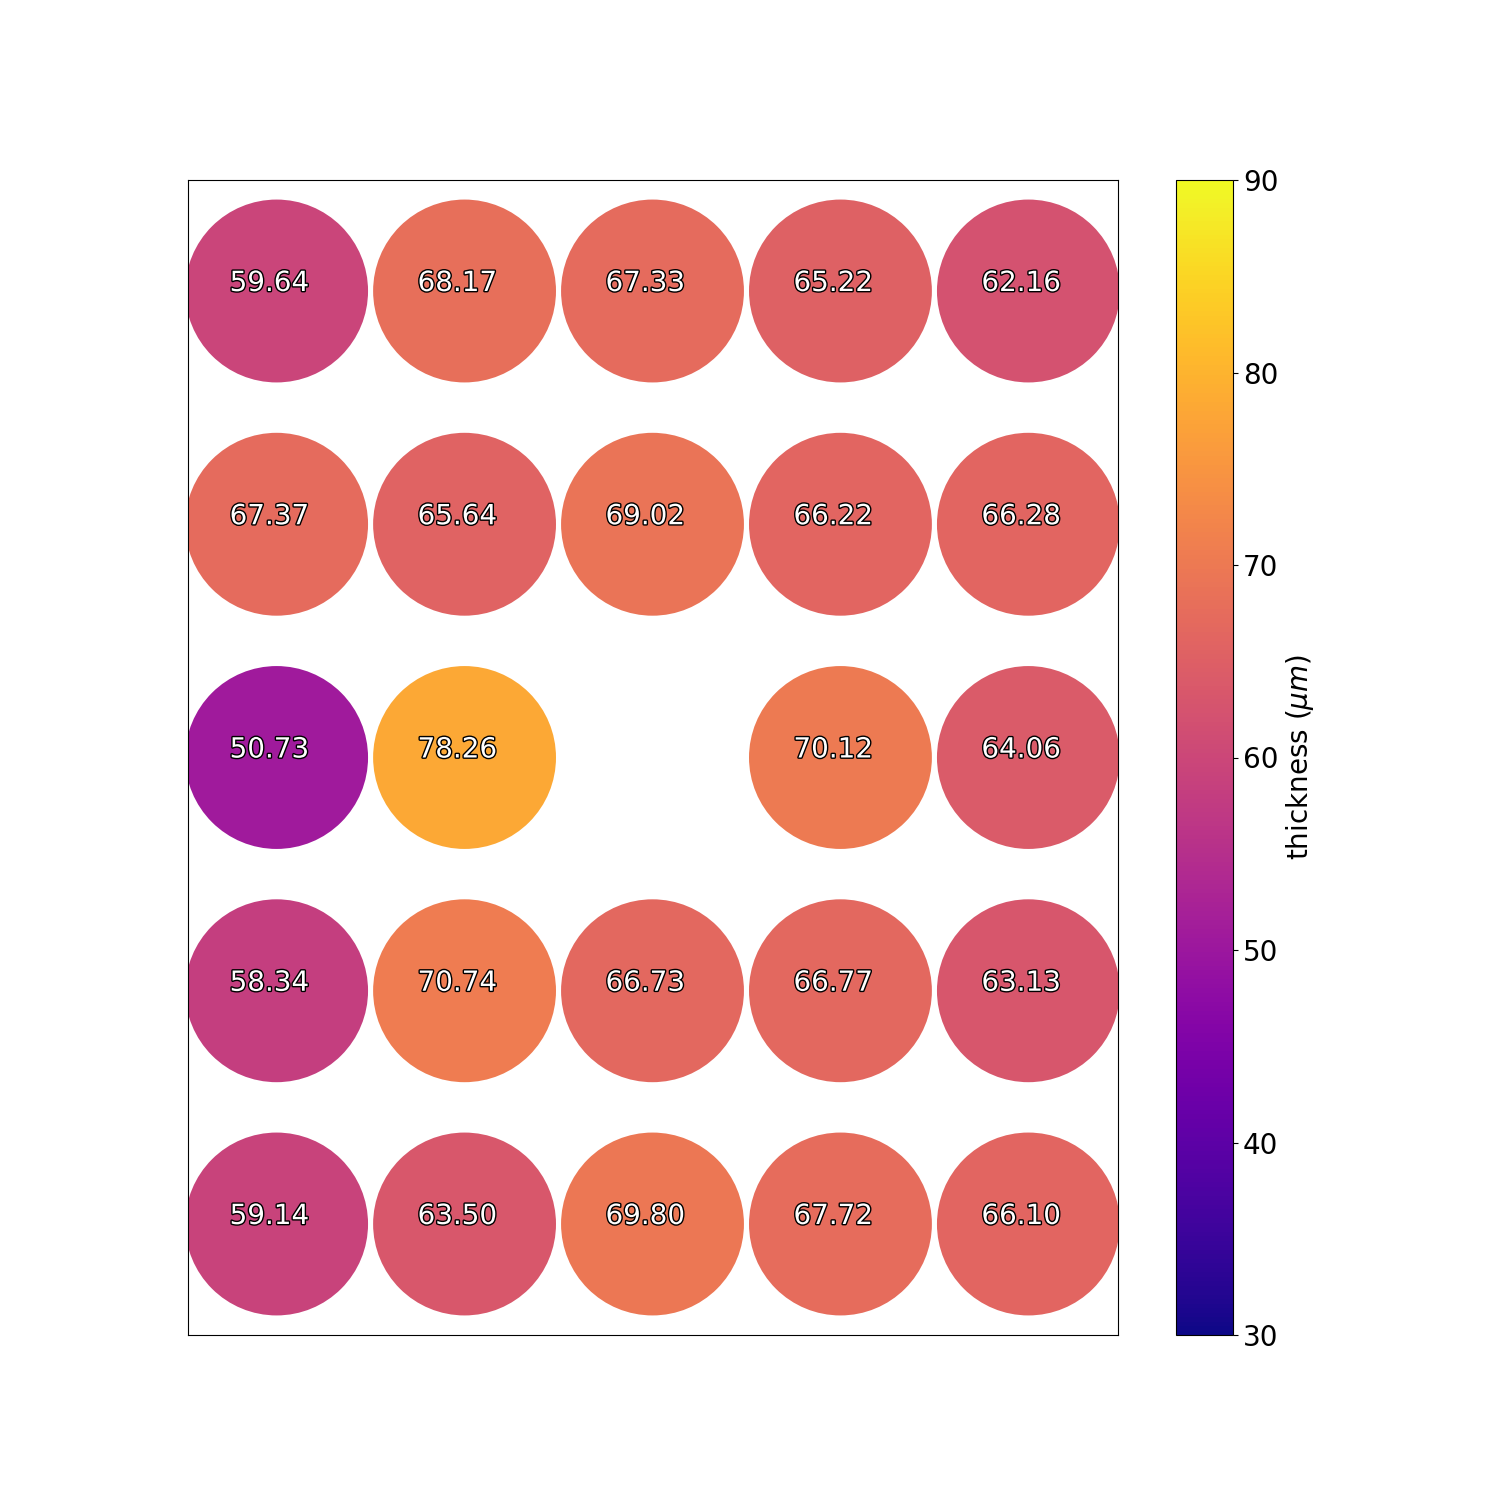
\includegraphics[width=\textwidth,keepaspectratio]{2D_copper_thickness_distri.png}
                        \caption{Visualisation de la variation d'épaisseur de cuivre d'un \gls{lem} mesurée à travers les 24 trous de la plaque d'acier.}
                        \label{fig::distri_24_trou_cuivre_2D}
                    \end{subfigure}\\
                    \begin{subfigure}[b]{0.48\textwidth}
                        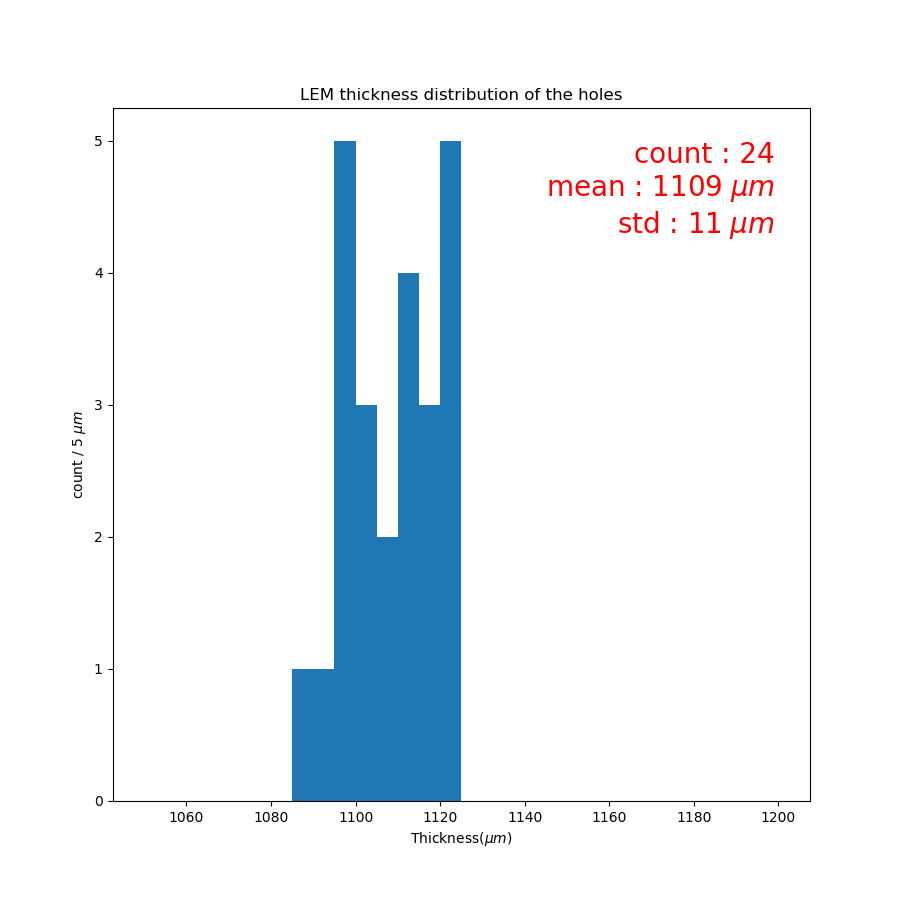
\includegraphics[width=\textwidth,keepaspectratio]{LEM.png}
                        \caption{Distribution de l'épaisseur totale d'un \gls{lem} mesurée à travers les 24 trous de la plaque d'acier.}
                        \label{fig::distri_24_trou_lem_1D}
                    \end{subfigure}
                    \hfill
                    \begin{subfigure}[b]{0.48\textwidth}
                        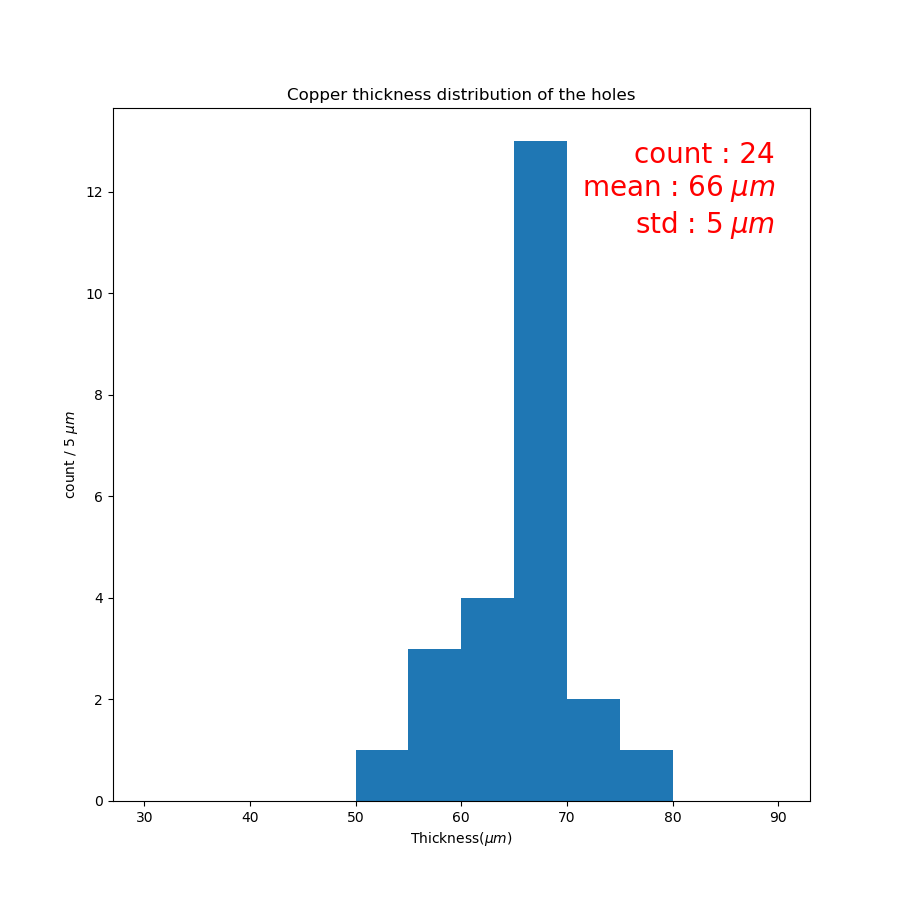
\includegraphics[width=\textwidth,keepaspectratio]{Copper.png}
                        \caption{Distribution de l'épaisseur de cuivre d'un \gls{lem} mesurée à travers les 24 trous de la plaque d'acier.}
                        \label{fig::distri_24_trou_cuivre_1D}
                    \end{subfigure}
                    \caption[Résultats des mesures d'épaisseur pour un \gls{lem}.]{Résultats des mesures d'épaisseur pour un \gls{lem}.}
                    \label{fig::distri_epaisseur_1_lem}
                \end{figure}
                
                \begin{figure}[htpb]
                    \begin{subfigure}[t]{0.48\textwidth}
                        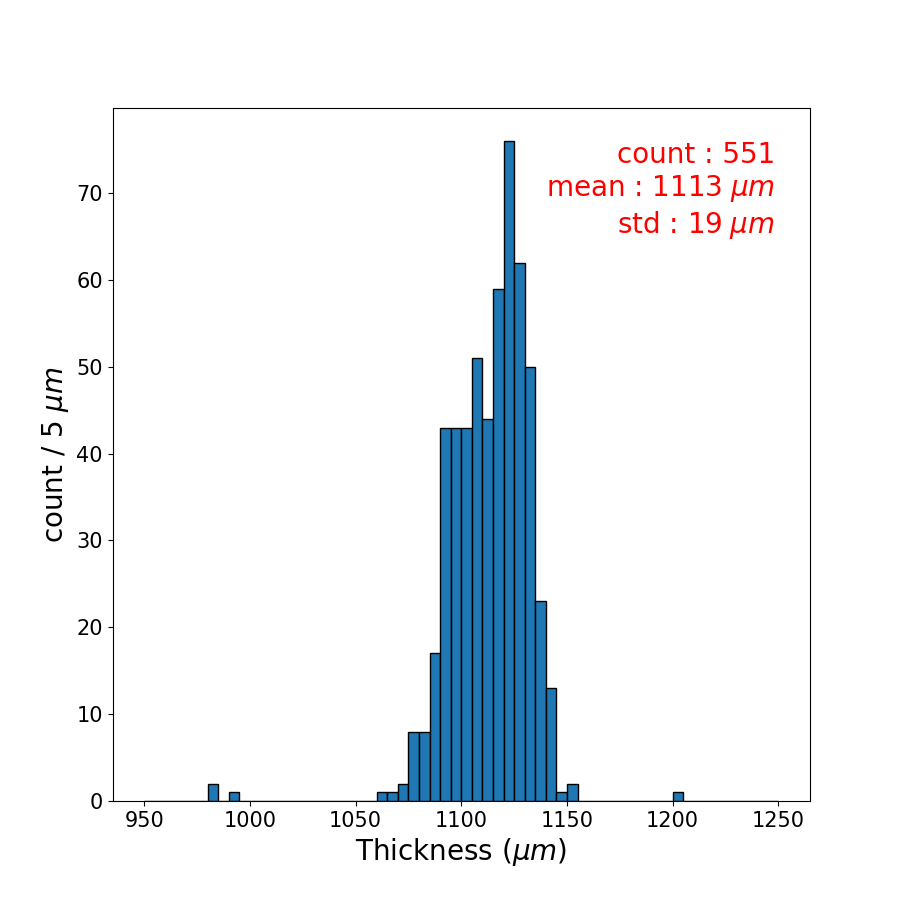
\includegraphics[width=\textwidth,keepaspectratio]{LEM_sum_all_histo_saclay.png}
                        \caption{Distribution de l'épaisseur totale de tous les \glspl{lem} du \gls{crp} 1 du démonstrateur 666 mesurée à travers les 24 trous de la plaque d'acier.}
                        \label{fig::distri_lem_saclay}
                    \end{subfigure}
                    \hfill
                    \begin{subfigure}[t]{0.48\textwidth}
                        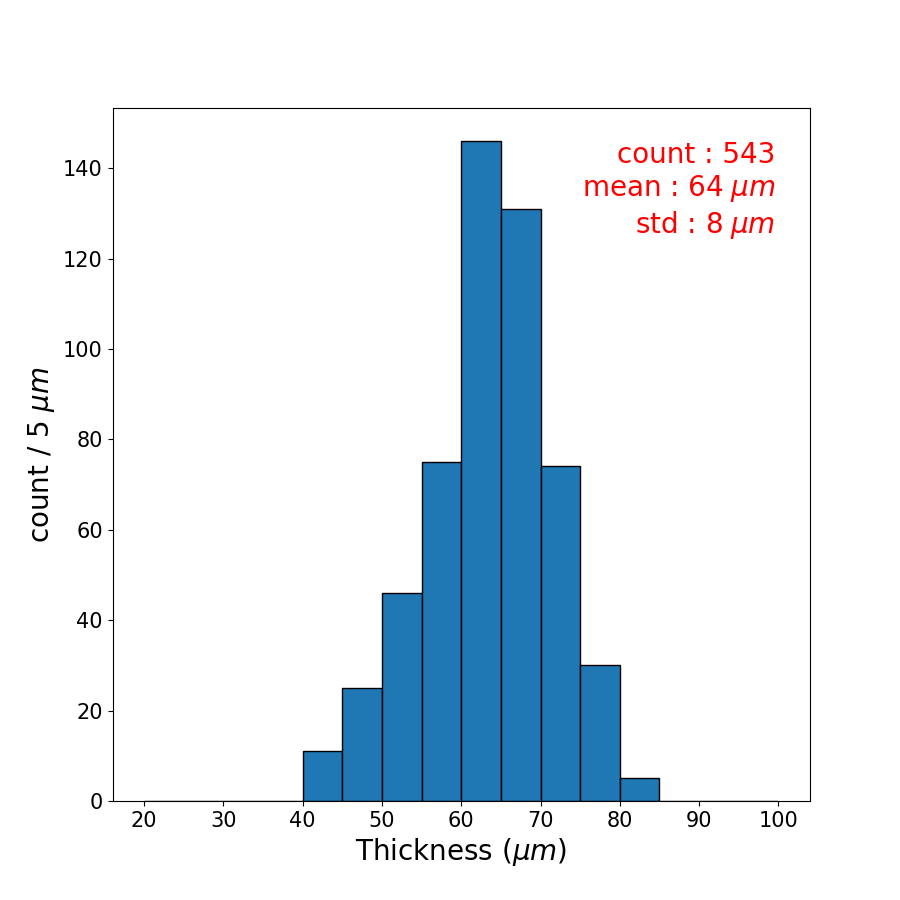
\includegraphics[width=\textwidth,keepaspectratio]{Copper_sum_all_histo_saclay.png}
                        \caption{Distribution de l'épaisseur de cuivre de tous les \glspl{lem} du \gls{crp} 1 du démonstrateur 666 mesurée à travers les 24 trous de la plaque d'acier.}
                        \label{fig::distri_cuivre_saclay}
                    \end{subfigure}\\
                    \begin{subfigure}[b]{0.48\textwidth}
                        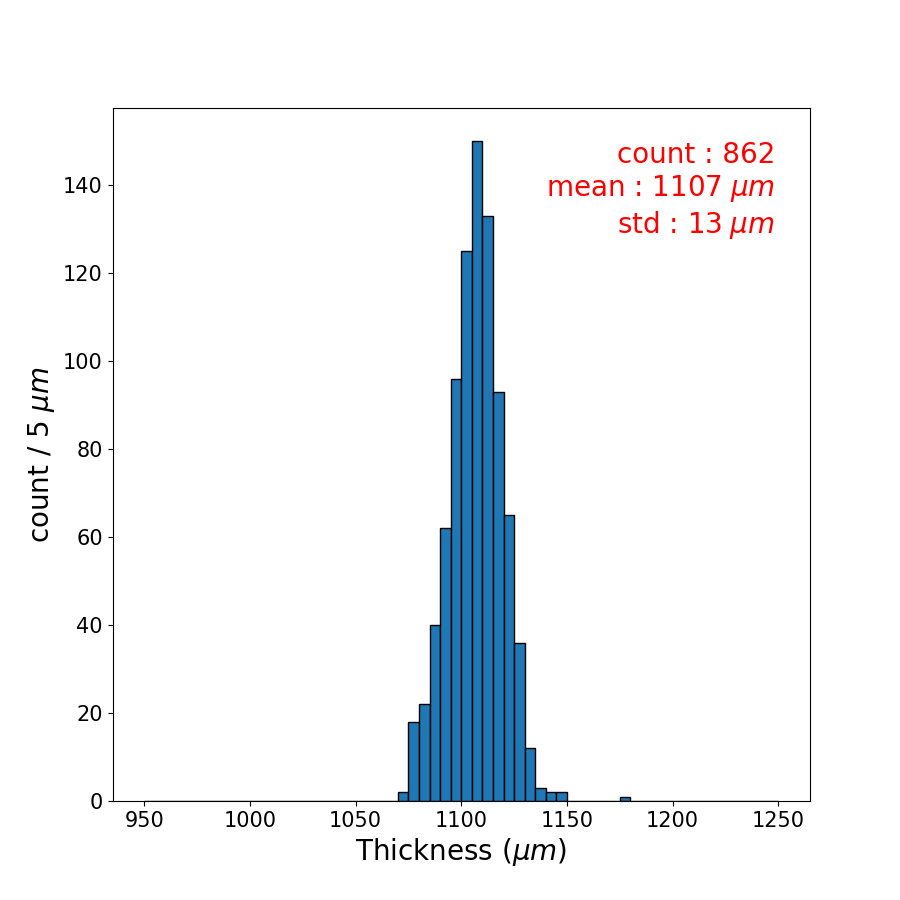
\includegraphics[width=\textwidth,keepaspectratio]{LEM_sum_all_histo_cern.png}
                        \caption{Distribution de l'épaisseur totale de tous les \glspl{lem} du \gls{crp} 2 du démonstrateur 666 mesurée à travers les 24 trous de la plaque d'acier.}
                        \label{fig::distri_lem_cern}
                    \end{subfigure}
                    \hfill
                    \begin{subfigure}[b]{0.48\textwidth}
                        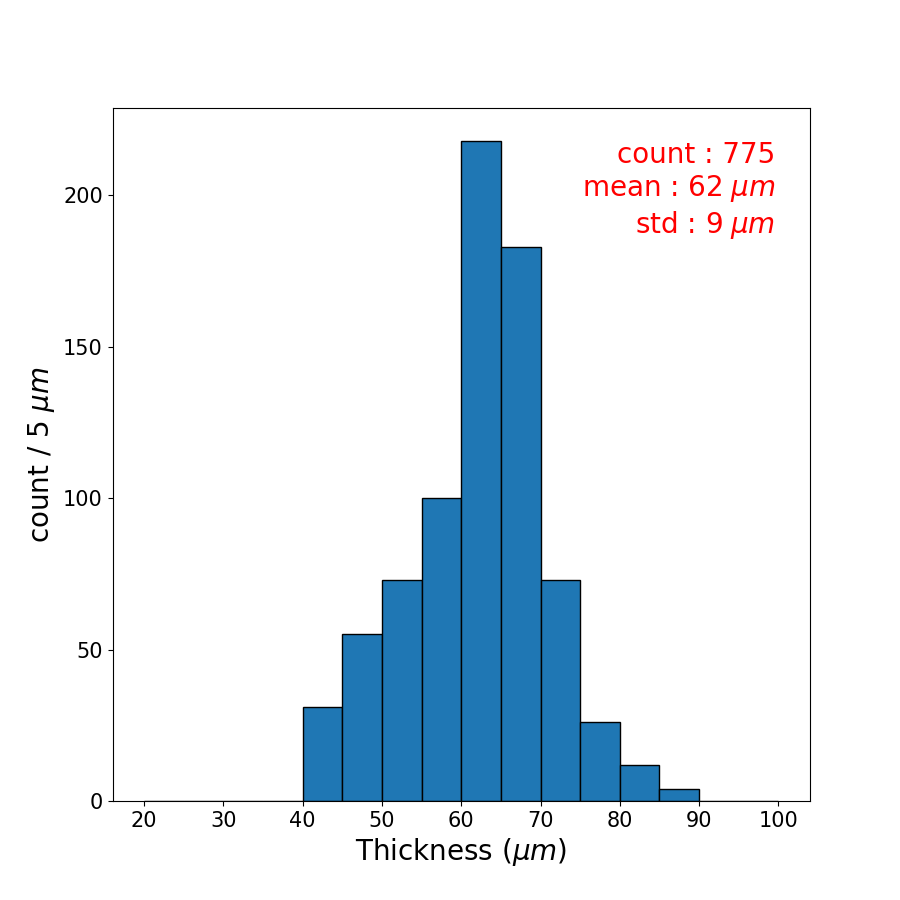
\includegraphics[width=\textwidth,keepaspectratio]{Copper_sum_all_histo_cern.png}
                        \caption{Distribution de l'épaisseur de cuivre de tous les \glspl{lem} du \gls{crp} 2 du démonstrateur 666 mesurée à travers les 24 trous de la plaque d'acier.}
                        \label{fig::distri_cuivre_cern}
                    \end{subfigure}
                    \caption[Résultats des mesures d'épaisseur pour tous les \glspl{lem}.]{Résultats des mesures d'épaisseur pour tous les \glspl{lem}. La première ligne correspond aux \glspl{lem} du \gls{crp} 1 du démonstrateur 666, la seconde ligne correspond aux \glspl{lem} du \gls{crp} 2 du démonstrateur 666.}
                    \label{fig::epaisseur_tous_lem}
                \end{figure}
                
                \begin{figure}[htpb]
                    \begin{subfigure}[t]{0.48\textwidth}
                        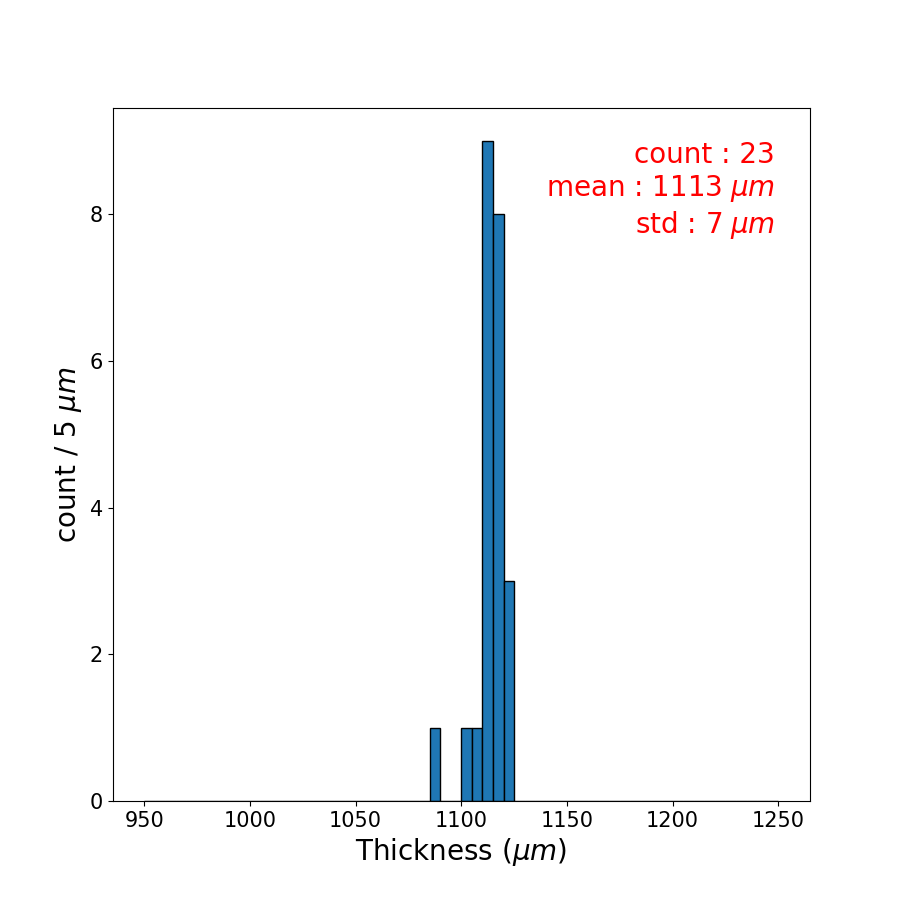
\includegraphics[width=\textwidth,keepaspectratio]{LEM_means_sum_all_histo_saclay.png}
                        \caption{Distribution de l'épaisseur de totale moyennée sur les 24 trous de mesure d'un \gls{lem} pour tous les \glspl{lem} du \gls{crp} 1 du démonstrateur 666. Seuls \numprint{22} des \numprint{36} \glspl{lem} ont été mesurés.}
                        \label{fig::distri_moyenne_lem_saclay}
                    \end{subfigure}
                    \hfill
                    \begin{subfigure}[t]{0.48\textwidth}
                        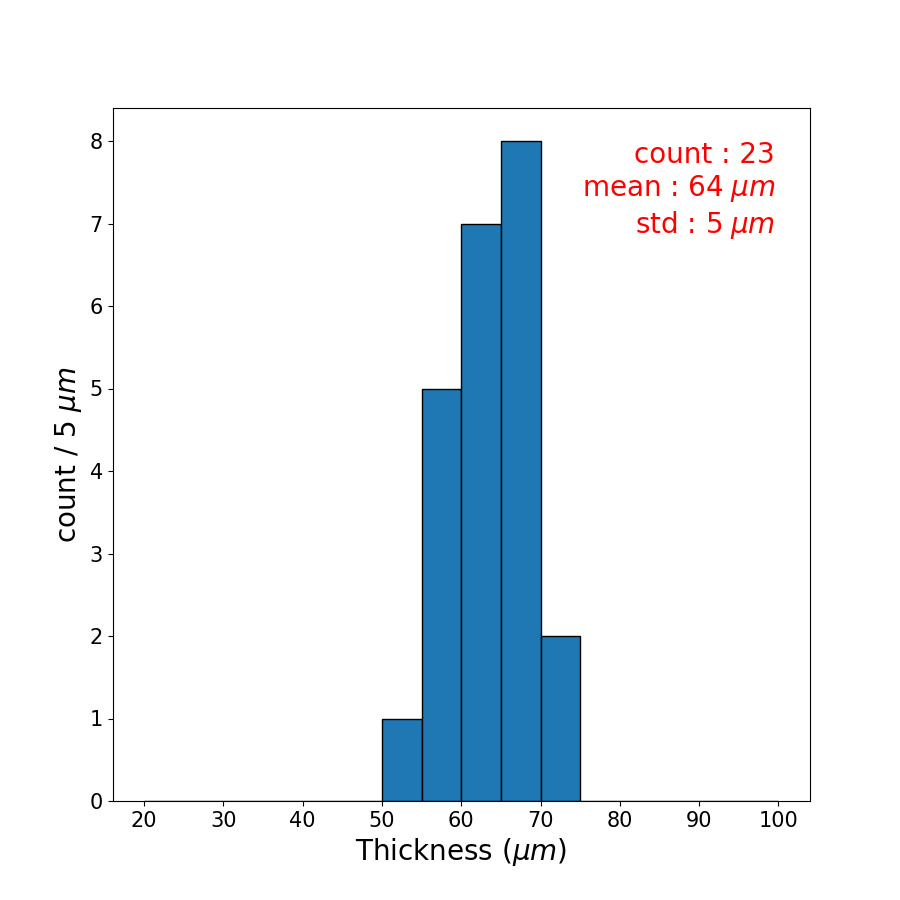
\includegraphics[width=\textwidth,keepaspectratio]{Copper_means_sum_all_histo_saclay.png}
                        \caption{Distribution de l'épaisseur de cuivre moyennée sur les 24 trous de mesure d'un \gls{lem} pour tous les \glspl{lem} du \gls{crp} 1 du démonstrateur 666. Seuls \numprint{22} des \numprint{36} \glspl{lem} ont été mesurés}
                        \label{fig::distri_moyenne_cuivre_saclay}
                    \end{subfigure}\\
                    \begin{subfigure}[b]{0.48\textwidth}
                        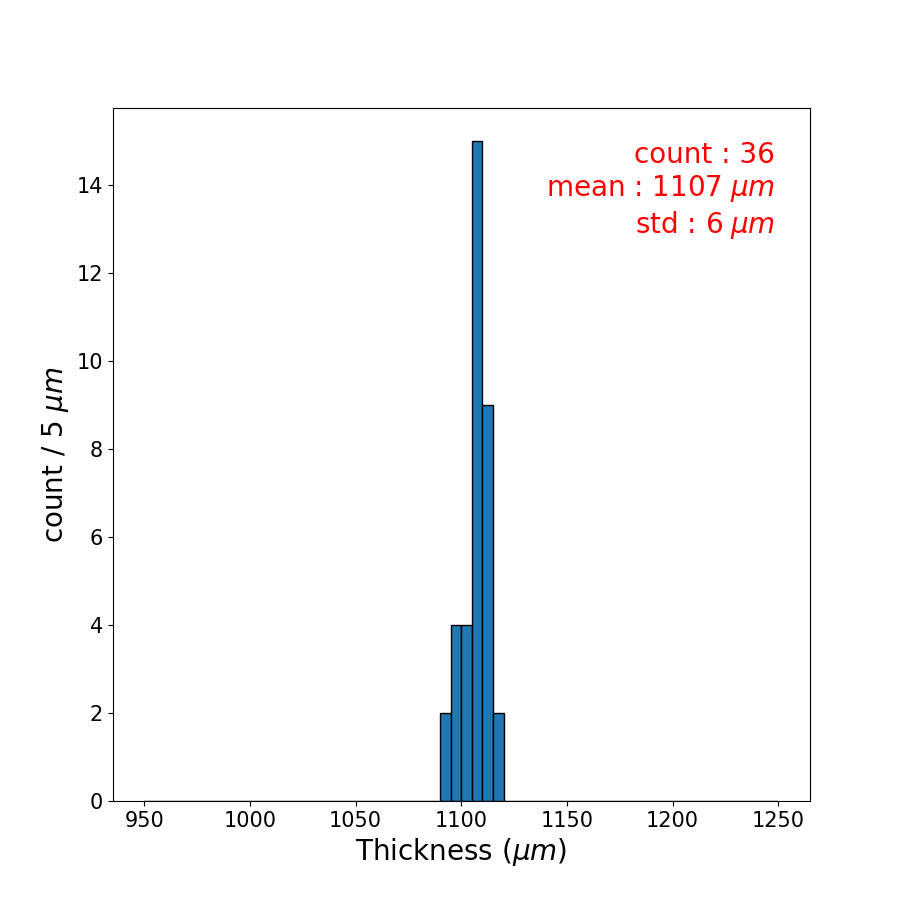
\includegraphics[width=\textwidth,keepaspectratio]{LEM_means_sum_all_histo_cern.png}
                        \caption{Distribution de l'épaisseur de totale moyennée sur les 24 trous de mesure d'un \gls{lem} pour tous les \glspl{lem} du \gls{crp} 2 du démonstrateur 666.}
                        \label{fig::distri_moyenne_lem_cern}
                    \end{subfigure}
                    \hfill
                    \begin{subfigure}[b]{0.48\textwidth}
                        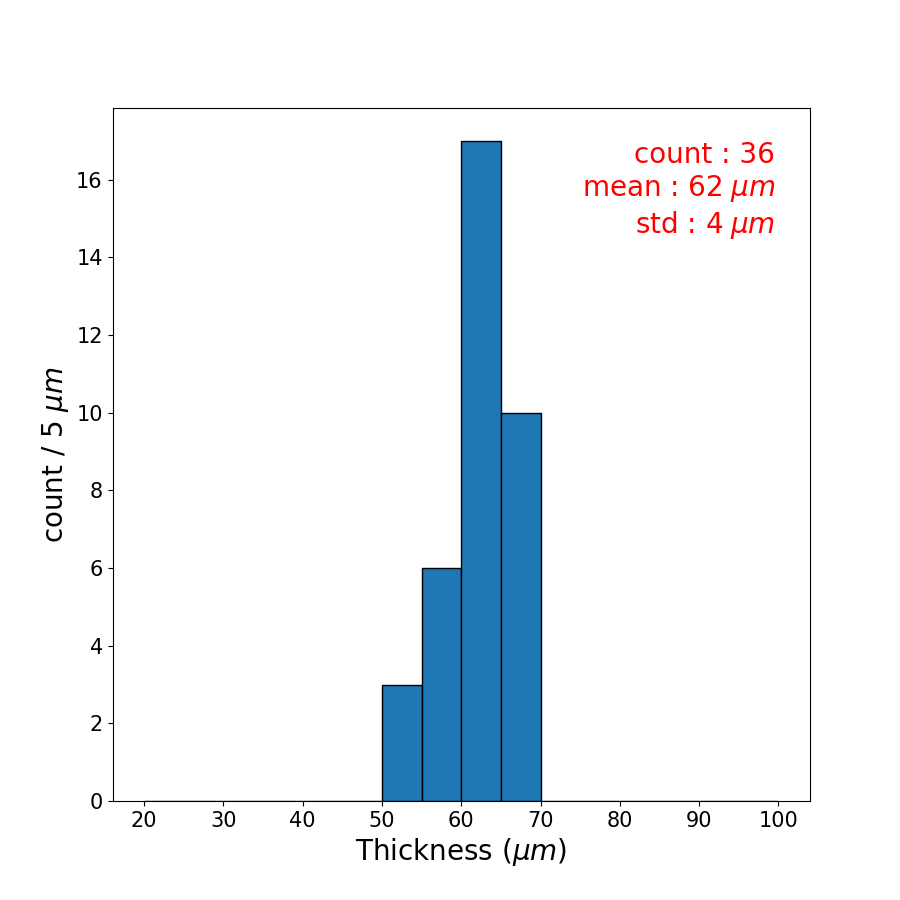
\includegraphics[width=\textwidth,keepaspectratio]{Copper_means_sum_all_histo_cern.png}
                        \caption{Distribution de l'épaisseur de cuivre moyennée sur les 24 trous de mesure d'un \gls{lem} pour tous les \glspl{lem} du \gls{crp} 2 du démonstrateur 666.}
                        \label{fig::distri_moyenne_cuivre_cern}
                    \end{subfigure}
                    \caption[Résultats des mesures d'épaisseurs moyennées sur les 24 trous de mesure pour tous les \glspl{lem}.]{Résultats des mesures d'épaisseur moyennée sur les 24 trous de mesure pour tous les \glspl{lem}. La première ligne correspond aux \glspl{lem} du \gls{crp} 1 du démonstrateur 666, la seconde ligne correspond aux \glspl{lem} du \gls{crp} 2 du démonstrateur 666.}
                    \label{fig::epaisseur_moyenne_tous_lem}
                \end{figure}
            
                \begin{figure}[htbp]
                    \begin{subfigure}[t]{0.48\textwidth}
                        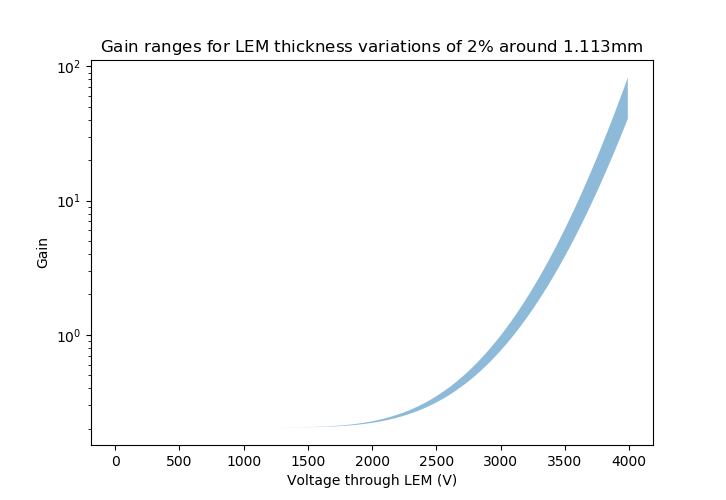
\includegraphics[width=\textwidth,keepaspectratio]{exp_gain_range_from_measurements.png}
                        \caption{Variation attendues du gain pour une épaisseur de \gls{lem} de $\SI{1113}{\micro\meter}\pm2\%$.}
                    \end{subfigure}
                    \hfill
                    \begin{subfigure}[t]{0.48\textwidth}
                        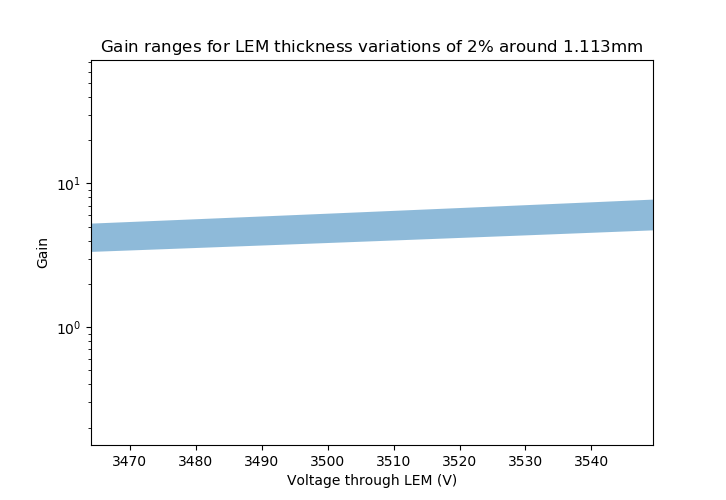
\includegraphics[width=\textwidth,keepaspectratio]{exp_gain_range_from_measurements_zoom.png}
                        \caption{Variation attendues du gain pour une épaisseur de \gls{lem} de $\SI{1113}{\micro\meter}\pm2\%$, agrandissement autour de \SI{35}{\kilo\volt\per\centi\meter}.}
                    \end{subfigure}
                    \caption[Variation attendues du gain pour une épaisseur de \gls{lem} de $\SI{1113}{\micro\meter}\pm2\%$.]{Variation attendues du gain pour une épaisseur de \gls{lem} de $\SI{1113}{\micro\meter}\pm2\%$, d'après le formule \eqref{eq::townsend_avalanche_2} ajustée aux données présentées dans \cite{Cantini2014}.}
                    \label{fig::exp_gain_range}
                \end{figure}
                
                \begin{wrapfigure}{r}{0.4\textwidth}
                    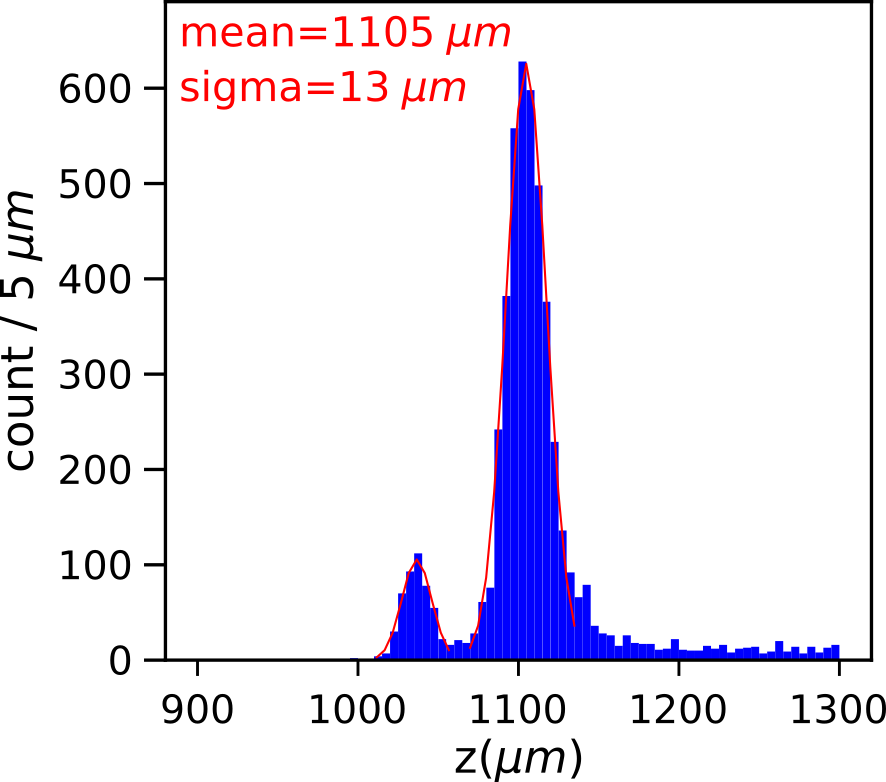
\includegraphics[width=0.4\textwidth,keepaspectratio]{distri_1_trou_lem.png}
                    \caption[Distribution de l'épaisseur d'un \gls{lem} mesurée à travers u trou de la plaque en acier.]{Distribution de l'épaisseur d'un \gls{lem} mesurée à travers un trou de la plaque en acier. L'ajustement gaussien de gauche correspond au \gls{fr4}, celui de droite au cuivre.}
                    \label{fig::distri_1_trou_lem}
                \end{wrapfigure}
                
                Les distributions des hauteurs dans les 24 trous de mesure du \gls{lem} sont tracées avec correction pour la pente du marbre. La \autoref{fig::distri_1_trou_lem} montre une telle distribution pour un trou de mesure. Une double gaussienne y est ajustée afin de déterminer l'épaisseur totale $E_T$ du \gls{lem} ainsi que l'épaisseur $E_C$ du cuivre. La moyenne de la gaussienne la plus à droite sur la \autoref{fig::distri_1_trou_lem} correspond à l'épaisseur totale $E_T$ du \gls{lem}, tandis que la moyenne de la gaussienne la plus à gauche correspond à $E_T - E_C$, en supposant que l'épaisseur du cuivre est la même sur chaque face. $E_C$ est alors calculable facilement, de même que l'épaisseur de \gls{fr4} $E_F$ car nous avons la relation $E_T = E_F + 2E_C$.
                
                A noter que les mesures ne permettaient pas toujours de d'ajuster deux gaussiennes. Dans certains cas, seul l'épaisseur totale était accessible, il y a donc moins de statistiques dans les histogrammes des épaisseurs de cuivre et de \gls{fr4}.
                
                La \autoref{fig::distri_epaisseur_1_lem} montre les distributions de l'épaisseur total et de l'épaisseur de cuivre pour les 24 trous de mesure d'un \gls{lem}. Afin d'estimer les variations attendues du gain sur les deux \glspl{crp} du démonstrateur 666, la distribution de ces épaisseurs mesurées dans chaque trou de mesure des \glspl{lem} de chaque \gls{crp} est montrée en \autoref{fig::epaisseur_tous_lem}. La \autoref{fig::exp_gain_range} montre les variations attendues du gain pour une épaisseur de \gls{lem} de $\SI{1113}{\micro\meter}\pm2\%$, correspondant au \gls{crp} 1 du démonstrateur. À \SI{3.5}{\kilo\volt}, la variation est de l'ordre de $20\%$.
                
                La \autoref{fig::epaisseur_moyenne_tous_lem} montre la distributions des épaisseurs totales et des épaisseurs de cuivre moyennées sur les 24 trous de chaque \gls{lem} pour les deux \gls{crp}. Elle permet de comparer nos mesures à celles d'ELTOS, qui ne réalisait que 2 mesures par \gls{lem} pour l'épaisseur de cuivre et 4 pour l'épaisseur totale. 
                
            \subsubsection{Comparaison aux mesures faites par ELTOS}\label{sec::thickness_comparison_eltos}
            
                \begin{figure}[htpb]
                    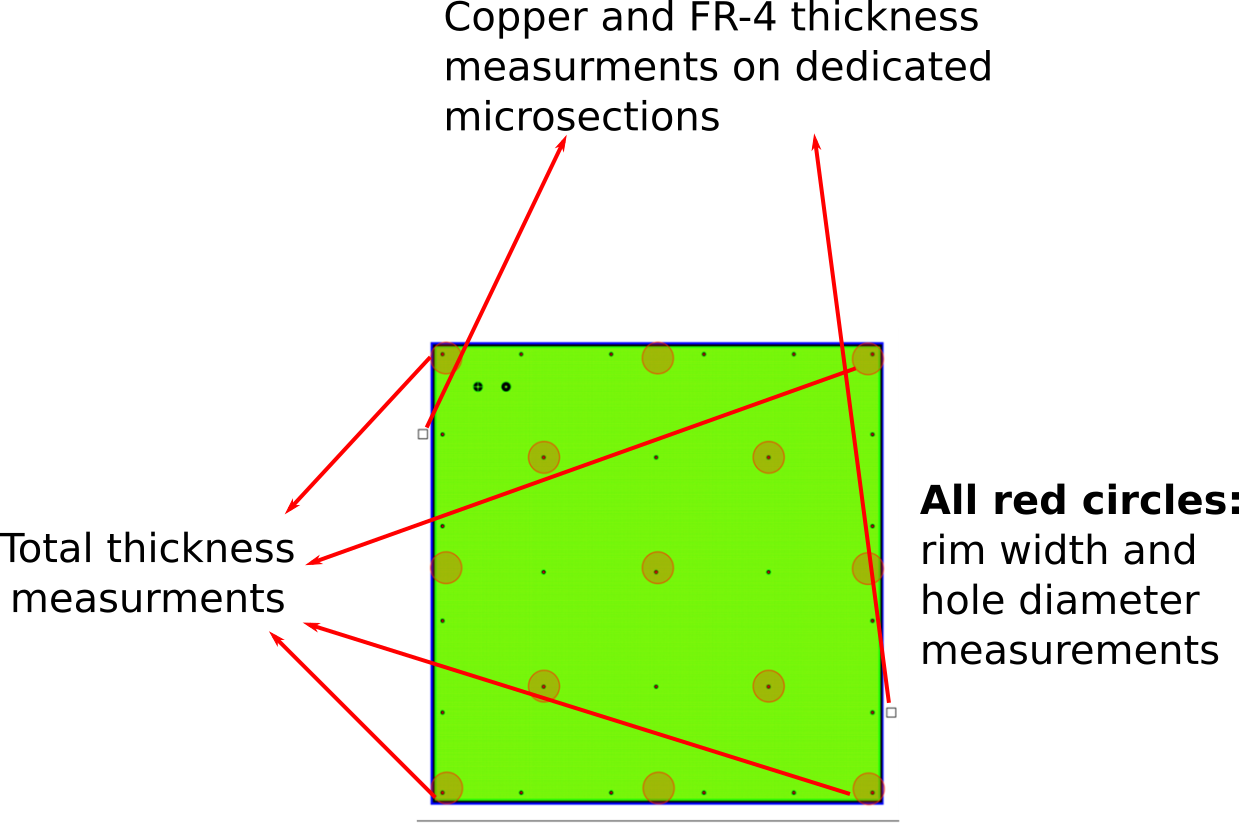
\includegraphics[width=0.8\textwidth]{eltos_measurement.png}
                    \caption[zones de mesure des caractéristiques géométriques d'un \gls{lem}]{Gerber d'un \gls{lem} avec indiquées en rouges les zones de mesure des caractéristiques géométriques pour vérification de la concordance au cahier des charges présenté en \autoref{sec::LEM}}
                    \label{fig::mesures_eltos}
                \end{figure}
            
                La \autoref{fig::mesures_eltos} montre les zones du \gls{lem} où ELTOS a mesuré les différentes caractéristiques géométriques : la taille totale, l'épaisseur totale, l'épaisseur de cuivre, l'épaisseur de \gls{fr4}, l'épaisseur des rims et le diamètre des trous. Les épaisseurs de cuivre et de \gls{fr4} été mesurées en deux points situés sur les coins des \glspl{lem}, donnant une statistique de $2\times36=72$ pour les moyennes et écart type chaque \gls{crp} du démonstrateur 666. L'épaisseur totale était mesurée a quatre coins, donnant une statistique de 144 pour chaque \gls{crp}. L'épaisseur du rim et le diamètre des trous était mesurés en treize points, donnant une statistique de 468 chacun pour chaque \gls{crp}.
                
                Due à la faible statistique des épaisseur de cuivre et des épaisseur totales, la comparaison au mesures faites à Saclay est faite avec les distributions des moyennes sur tout le \gls{lem} des mêmes épaisseurs. Le \autoref{tab::mesures_eltos} résume ces résultats et indique ceux obtenus à Saclay.
                
                \begin{table}
                \centering
                \begin{tabular}{|l|c|c||c|c|}
                    \hline
                    \gls{crp} 1 & Moyenne ELTOS & Écart type ELTOS & Moyenne \gls{cci} & Écart type \gls{cci}\\
                    \hline
                    Épaisseur d'époxy & \SI{0.97}{\milli\meter} & \SI{0.01}{\milli\meter} & &\\
                    Épaisseur de cuivre & \SI{97}{\micro\meter} & \SI{1.88}{\micro\meter} & \SI{64}{\micro\meter} & \SI{5}{\micro\meter}\\
                    Épaisseur totale & \SI{1.12}{\milli\meter} &  \SI{0.005}{\milli\meter} & \SI{1.11}{\milli\meter} &  \SI{0.007}{\milli\meter}\\
                    Largeur du rim (haut)& \SI{41}{\micro\meter} & \SI{1.6}{\micro\meter} & &\\
                    Largeur du rim (bas)& \SI{41}{\micro\meter} & \SI{1.6}{\micro\meter} & &\\
                    Surface totale &  $499.43\times\SI{499.43}{\milli\meter\squared}$ & \SI{0.03}{\milli\meter} & &\\
                    Diamètre des trous & $\SI{0.500}{\milli\meter}$ & \SI{1}{\micro\meter} & &\\
                     \hline
                \end{tabular}\\
                \begin{tabular}{|l|c|c||c|c|}
                    \hline
                    \gls{crp} 2 & Moyenne ELTOS & Écart type ELTOS & Moyenne \gls{cci} & Écart type \gls{cci}\\
                    \hline
                    Épaisseur d'époxy & \SI{0.97}{\milli\meter} & \SI{0.01}{\milli\meter} & &\\
                    Épaisseur de cuivre & \SI{97}{\micro\meter} & \SI{1.88}{\micro\meter} & \SI{62}{\micro\meter} & \SI{4}{\micro\meter} \\
                    Épaisseur totale & \SI{1.12}{\milli\meter} &  \SI{0.005}{\milli\meter} & \SI{1.11}{\milli\meter} & \SI{0.006}{\milli\meter}\\
                    Largeur du rim (haut)& \SI{41}{\micro\meter} & \SI{1.6}{\micro\meter} & &\\
                    Largeur du rim (bas)& \SI{41}{\micro\meter} & \SI{1.6}{\micro\meter} & &\\
                    Surface totale &  $499.43\times\SI{499.43}{\milli\meter\squared}$ & \SI{0.03}{\milli\meter} & &\\
                    Diamètre des trous & $\SI{0.500}{\milli\meter}$ & \SI{1}{\micro\meter} & &\\
                     \hline
                \end{tabular}
                \caption[Mesures des différentes caractéristiques géométriques des \gls{lem}]{Mesures des différentes caractéristiques géométriques des \gls{lem} faites par ELTOS les deux \gls{crp} du démonstrateur 666, et comparaison aux mesures faites à Saclay avec la technique \gls{cci}.\label{tab::mesures_eltos}}
            \end{table}
            
            Les mesures réalisées par ELTOS et les mesures réalisées par le \gls{cea} sont compatibles pour les épaisseurs totales, mais il y a une différence notable concernant les mesures des moyennes des épaisseurs de cuivre et de \gls{fr4}. Une explication possible est que la technique \gls{cci} ne puisse pas estimer correctement les épaisseurs de cuivre due à la petite taille de la zone sur laquelle cette mesure peut s'effectuer, c'est à dire le rim de $40\micro\meter$. En effet, il est possible que certains rayons lumineux du crayon optique, qui ne devrait pas être focalisé sur la surface du \gls{fr4}, soit tout de même réfléchit par la parois en cuivre et soit détecté par le dispositif, faussant ainsi la distance mesurée. Cette explication n'affecte pas l'épaisseur totale du \gls{lem}.
        
        \subsection{Tests haute tension et mesures de gain}\label{sec::test_HT}
        
            \begin{figure}[htpb]
                \begin{subfigure}[t]{0.48\textwidth}
                    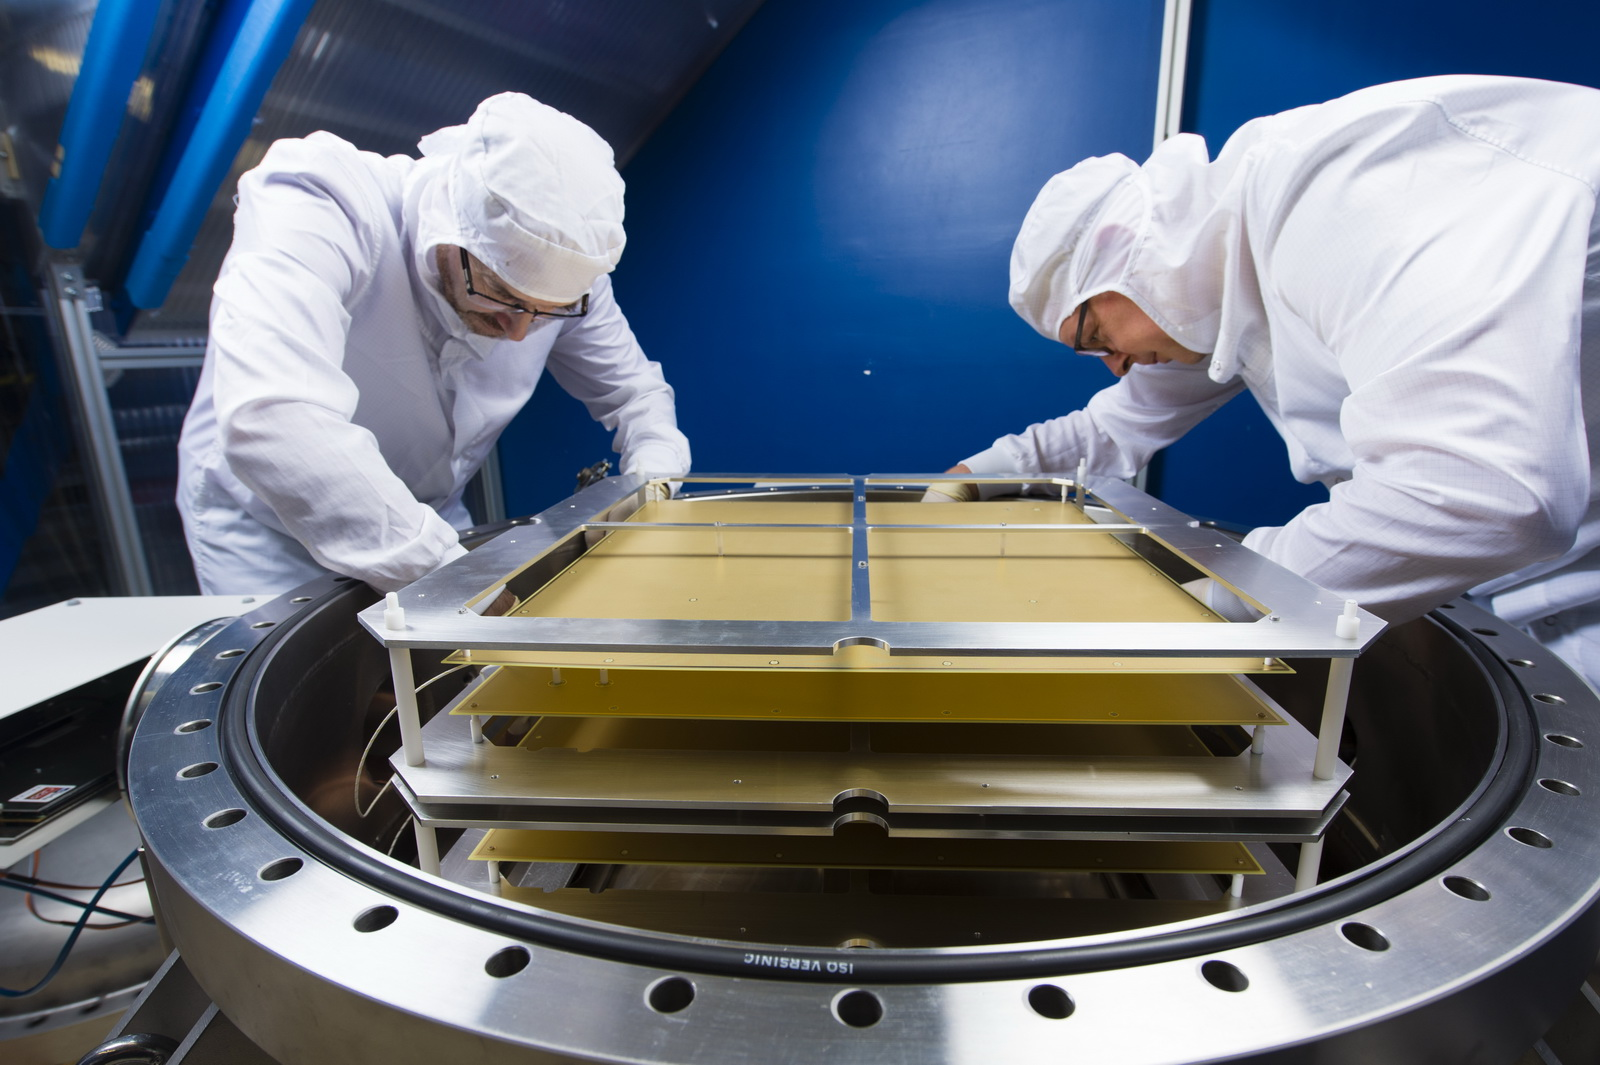
\includegraphics[width=\textwidth,keepaspectratio]{6lems_gamelle.jpg}
                    \caption{Chambre haute pression avec six \glspl{lem} en train d'être préparés pour un test de tenue en tesion.}
                    \label{fig::6lems_gamelle}
                \end{subfigure}
                \hfill
                \begin{subfigure}[t]{0.48\textwidth}
                    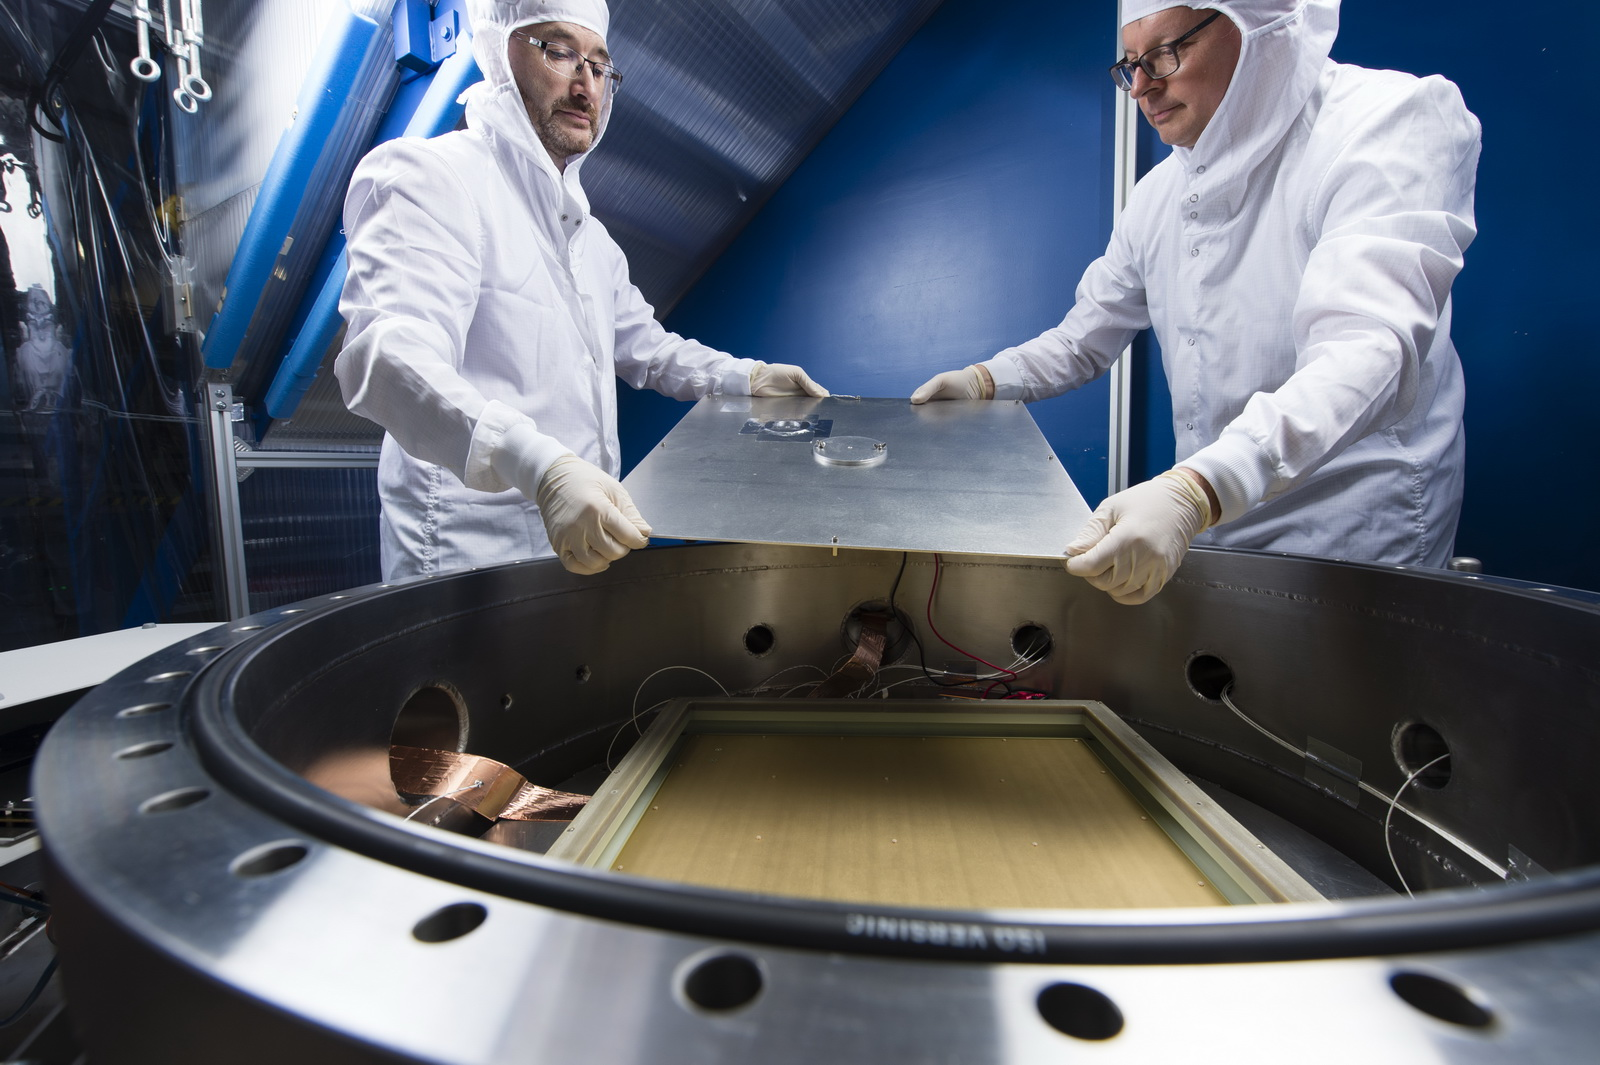
\includegraphics[width=\textwidth,keepaspectratio]{gamelle_source.jpg}
                    \caption{Chambre haute pression avec une source d'américium, un \gls{lem} et une anode en train d'être préparés pour une mesure de gain.}
                    \label{fig::gamelle_source}
                \end{subfigure}
                \caption[Chambre haute pression]{Chambre haute pression utilisée à Saclay pour les tests de tenue en tension et les mesures de gain des \glspl{lem} destinés au démonstrateur 666.}
                \label{fig::gamelle}
            \end{figure}

            \begin{wrapfigure}{r}{0.1\textwidth}
                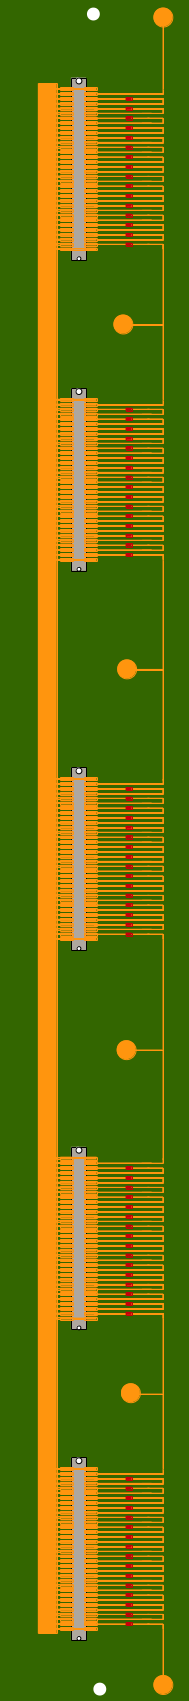
\includegraphics[width=0.1\textwidth,keepaspectratio]{Anode_Card_left.png}
                \caption[Schéma d'une carte de mesure utilisée pour les tests de continuité des anodes.]{Schéma d'une carte de mesure utilisée pour les tests de continuité des anodes.}
                \label{fig::Anode_Card_left}
            \end{wrapfigure}
            Une enceinte haute pression a été construite afin d'y recréer les conditions de pression et température des \gls{tpc} de \gls{wa105}\footnote{A noter que dans les \gls{tpc}, un gradient de température est présent, qui ne l'est pas dans l'enceinte haute pression.}. Tous les \glspl{lem} du démonstrateur 666 y ont été soumis à de hautes tensions afin de déterminer leur tension de claquage, et ce dans de l'air sec ainsi que dans de l'argon. A également été mesuré le gain de ces \glspl{lem} grâce à une source d'américium placée dans l'enceinte.
            
            Pour les tests haute tension, six \glspl{lem} pouvaient être testés en même temps. La \autoref{fig::6lems_gamelle} montre  ce dispositif. Pour les mesures de gains, un seul \gls{lem} était placé, ainsi qu'une anode de lecture et la source. L'espacement entre l'anode et le \gls{lem} est le même que sur le \gls{crp}, $\SI{2}{\milli\meter}$. La cathode avec la source est située $\SI{5}{\centi\meter}$ au dessus du \gls{lem}. La \autoref{fig::gamelle_source} montre ce dispositif.
        
        \subsection{Test de continuité des pistes des anodes}\label{sec::test_anode}
            \begin{figure}
                \begin{subfigure}[t]{0.48\textwidth}
                    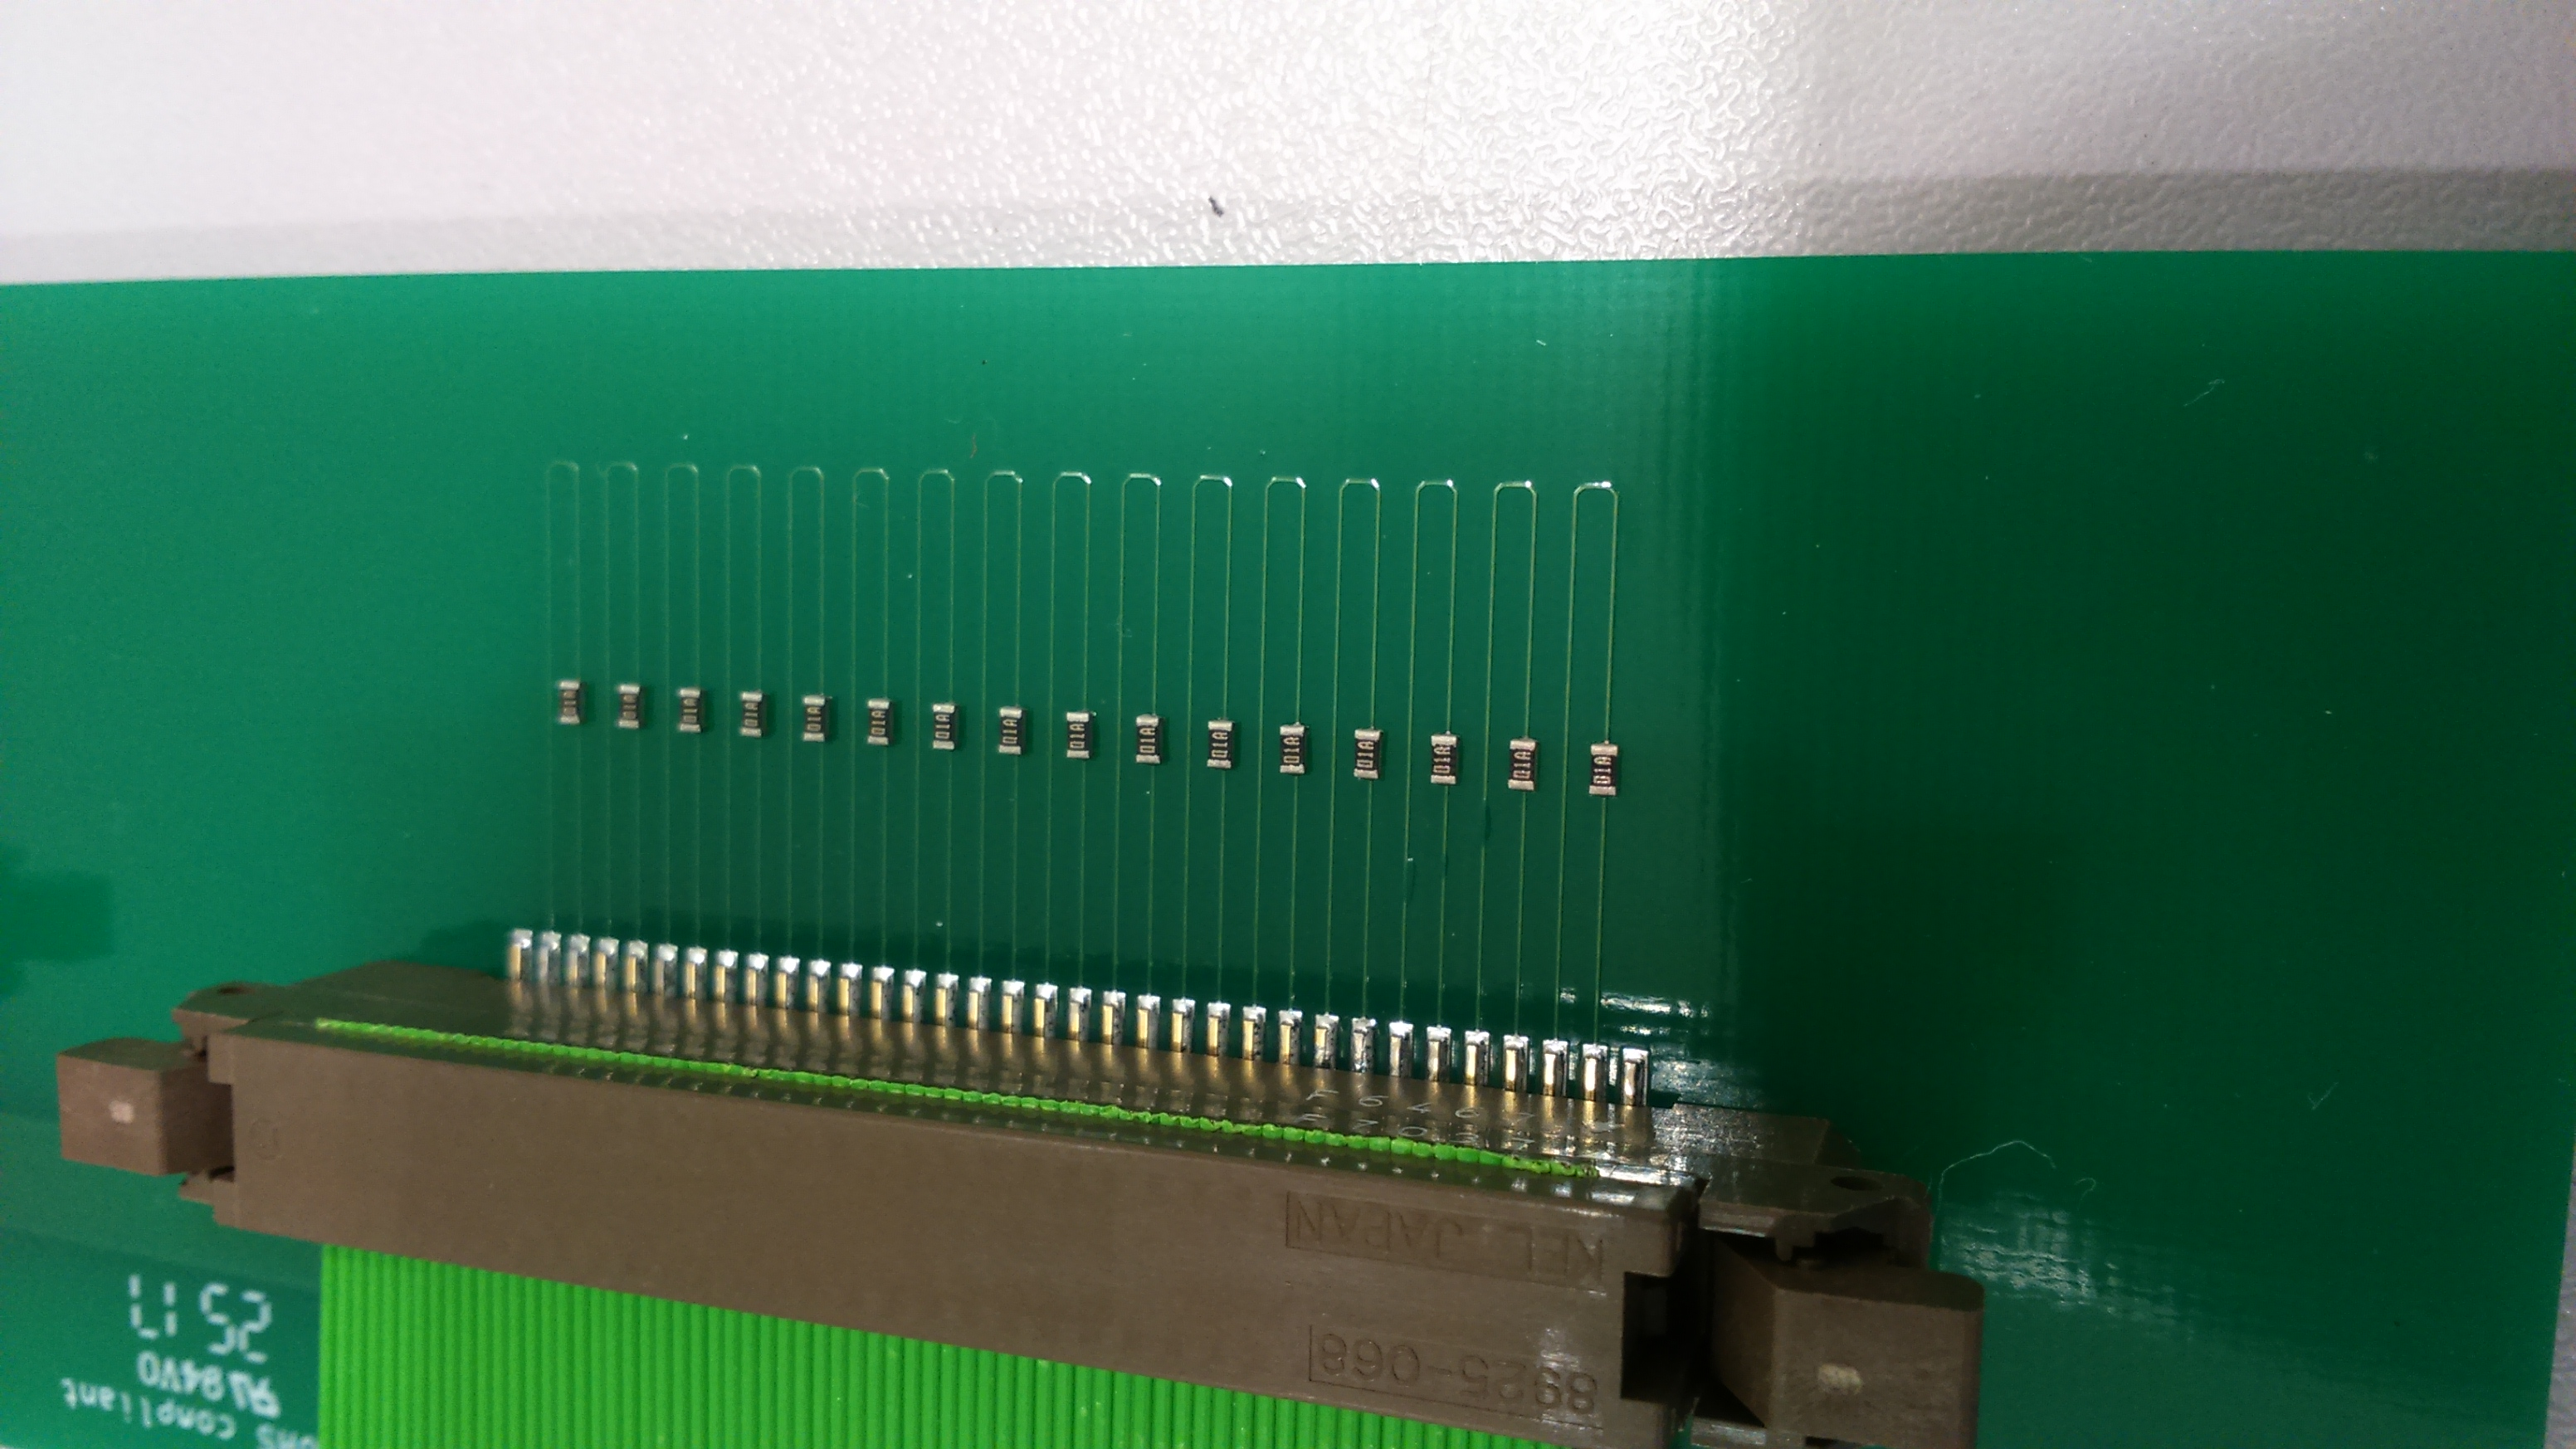
\includegraphics[width=\textwidth,keepaspectratio]{anode_card_zoom.JPG}
                    \caption{Agrandissement d'une carte de mesure. On y voit les résistances de \SI{100}{\ohm} placées entre les canaux de l'anode.}
                    \label{fig::anode_card_zoom}
                \end{subfigure}
                \hfill
                \begin{subfigure}[t]{0.48\textwidth}
                    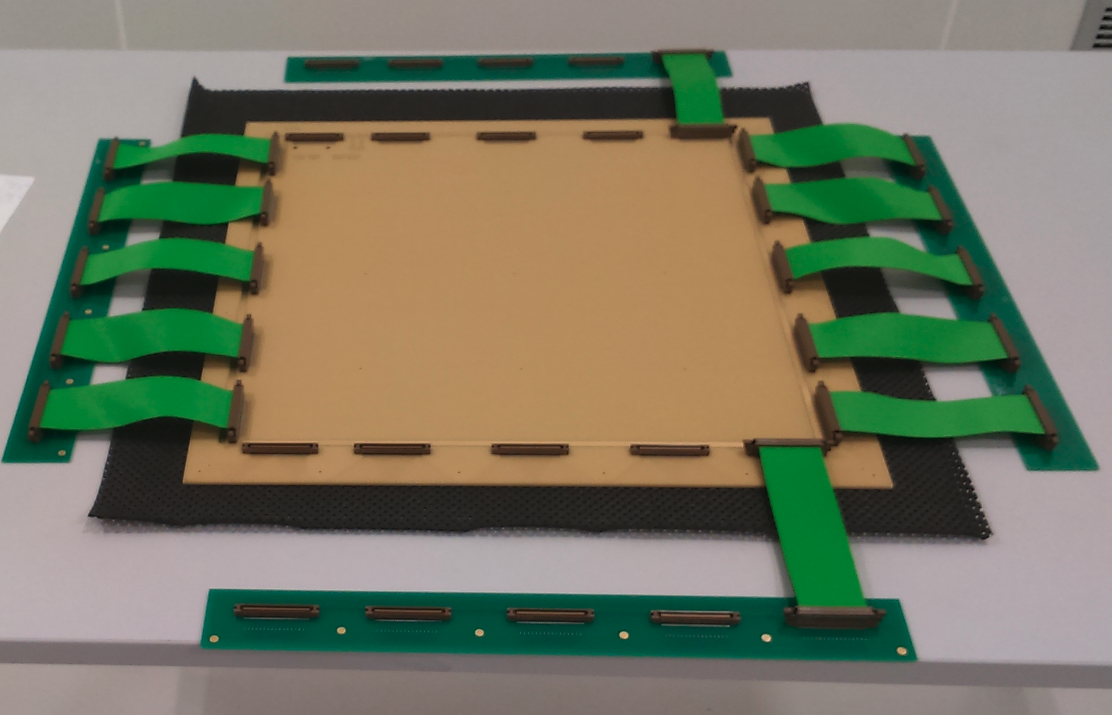
\includegraphics[width=\textwidth,keepaspectratio]{anode_carde.png}
                    \caption{Photo du dispositif de mesure. Les cartes de chaque côtés permettent aux \numprint{160} canaux de l'anode de n'en former plus qu'un, si aucun n'est cassé. Les cartes au dessus et au dessous servent à vérifier qu'il n'y a pas de court circuit entre les deux vues de l'anode.}
                    \label{fig::anode_card}
                \end{subfigure}
                \caption[Dispositif de mesure de la continuité des canaux des lecture des anodes.]{Dispositif de mesure de la continuité des canaux des lecture des anodes.}
                \label{fig::test_anode}
            \end{figure}
            La continuité des canaux de lecture des anodes, ainsi que leur isolation les unes par rapport aux autres, ont été testé grâce à des \gls{pcb} créé à cet effet (voir \autoref{fig::Anode_Card_left}. Deux jeux de deux cartes de test ont été produits et ont permit de vérifier les 72 anodes du démonstrateur 666 et 6 anodes de rab.
            
            Ces cartes sont munies des mêmes connecteurs que les anodes. Elles sont faites de manière à ce qu'en branchant une carte de chaque côté de l'anode, les 160 canaux d'une vue de l'anode forment un circuit continue. Des zones de cuivres sont prévus entre chaque groupe de 32 canaux d'y mesurer la résistance du groupe. La \autoref{fig::test_anode} montre le dispositif de mesure.

            \begin{wrapfigure}{r}{0.4\textwidth}
                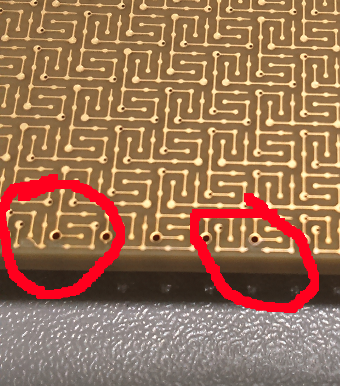
\includegraphics[width=0.4\textwidth,keepaspectratio]{anode_problem_zoom.png}
                \caption[Photo de canaux défaillant sur le bord d'une anode.]{Photo de canaux défaillant sur le bord d'une anode.}
                \label{fig::anode_test_probleme}
            \end{wrapfigure}
            Entre chaque canal est insérée une résistance de $\SI{100}{\ohm}$. Ainsi, une résistance de l'ordre de $\SI{3200}{\ohm}$ est attendue pour un groupe de 32 canaux. Une résistance significativement plus faible indiquera alors que deux ou plus canaux communiquent entre eux. Une résistance infinie indique un canal coupé. Dans les deux cas il s'agit alors de mesurer la résistance entre chaque canal du groupe posant problème afin d'identifier où se situe le problème, puis d'inspecter à l'oeil les pistes incriminées. La \autoref{fig::anode_test_probleme} montre de telles pistes.

            Au final, sur les 78 anodes ainsi testées, 10 ont posé problème. Parmi ces 10 anodes, 6 avaient des problèmes sur des canaux au bord de l'anode, où l'on ne s'attend de toute manière pas à collecter de charge à cause des zones mortes des \glspl{lem} (voir \autoref{sec::zones_mortes}).
                        
    \section{Efficacité d'extraction, probabilités de collection de charge}\label{sec::efficacites}
    
        La probabilité qu'a un électron d'être extrait de la phase liquide à la phase gazeuse a été étudiée dans les articles de E.M. Guschin et.al. (\cite{guschin}) et A.Bondar et.al. (\cite{Bondar2009}). Il a été montré que l'extraction se fait selon deux régimes : un rapide, de l'ordre de la nano-seconde, qui se traduit par une largeur de signal correspondant au temps caractéristique de l'électronique de lecture, et un lent (supérieur à la micro-seconde), qui se traduit par une largeur de signal supérieure au temps caractéristique de l'électronique de lecture. En pratique, les deux régimes sont présents et le signal est une composition des deux. Un champ d'extraction plus grand favorise la composante rapide, mais l'article \cite{Bondar2009} indique que dans l'argon pur, la composante lente reste dominante même à des champs d'extraction de $\SI{2}{\kilo\volt\per\centi\meter}$. Dans les détecteurs de \gls{wa105}, un événement est défini sur une plage temporelle de quelques centaines de micro-secondes, correspondant au temps nécessaires aux électrons de dérives pour parcourir toute la hauteur de la phase liquide. Un délai dans l'extraction de ces électrons de l'ordre de la dizaine de microsecondes peut avoir un impact significatif sur la forme du signal (voir \autoref{fig::extr_eff_on_waveform}), voir entraîner une perte significative de charge si le signal est mal reconstruit.
        
        Il existe également la possibilité qu'un électron, une fois extrait dans la phase gazeuse, n'atteignent pas la zone d'amplification des \glspl{lem}. En effet, des lignes de champ peuvent finir sur le \gls{fr4}, et ce des deux côtés du \gls{lem}. Cet effet, qui sera nommé \textit{probabilité de collection} dans le reste du texte, a été simulé en fonction du champ d'amplification et du champ d'extraction afin d'être également pris en compte dans l'estimation du gain. Le même phénomène peut également arriver après l'amplification : tous les électrons peuvent ne pas arriver à l'anode.
        
        \subsection{Méthodes de simulation}
        
            \begin{figure}[htpb]
                \begin{subfigure}[t]{0.48\textwidth}
                    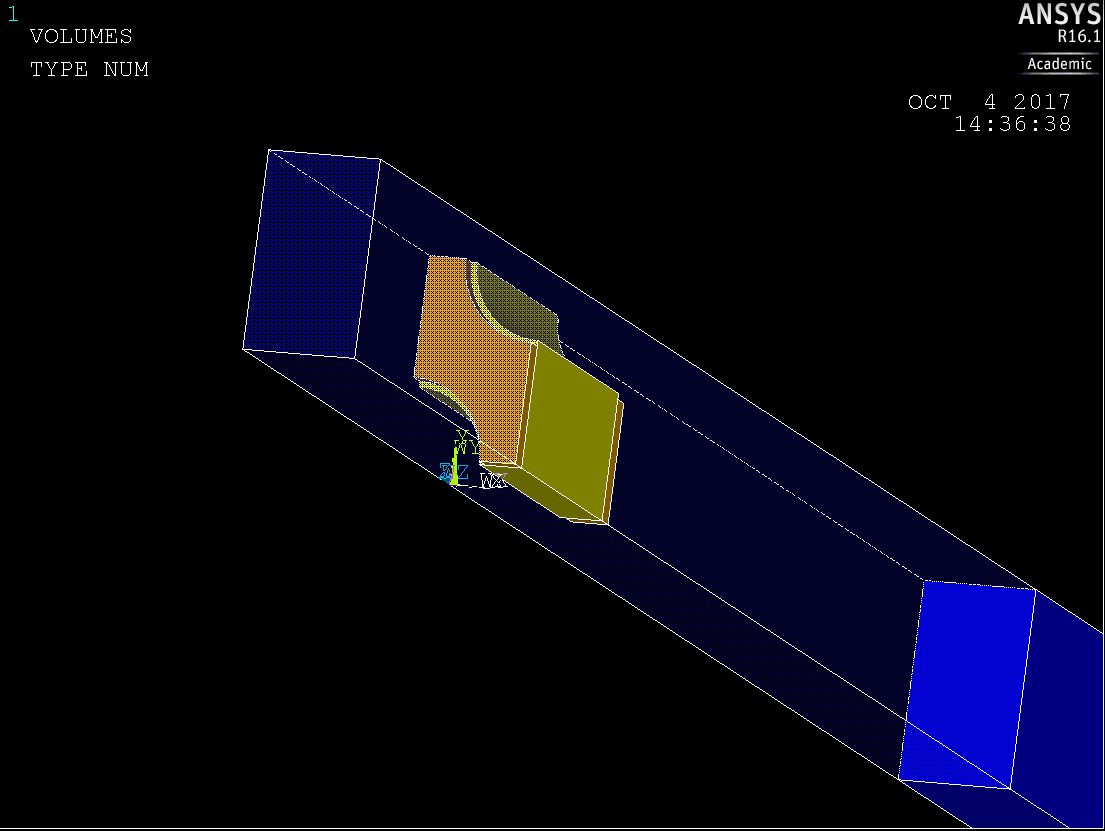
\includegraphics[width=\textwidth,keepaspectratio]{ansys_geom.png}
                \end{subfigure}
                \hfill
                \begin{subfigure}[t]{0.48\textwidth}
                    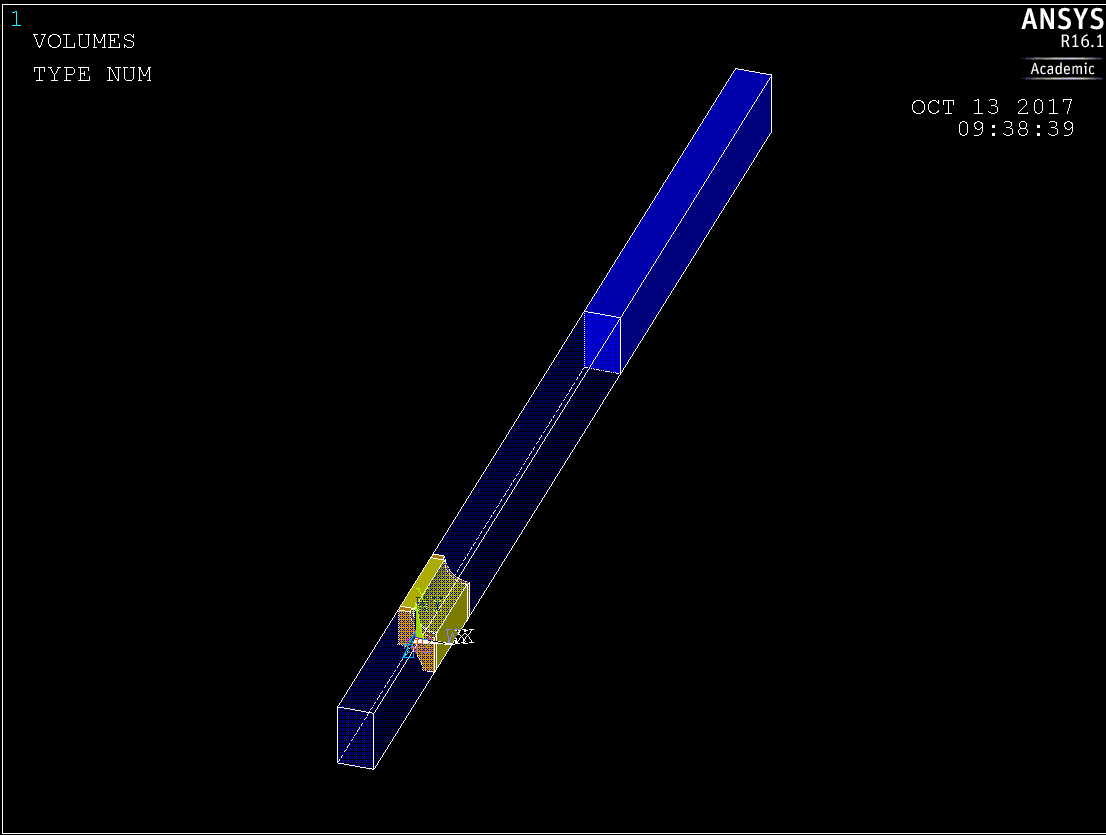
\includegraphics[width=\textwidth,keepaspectratio]{ansys_geom_unzoomed.png}
                \end{subfigure}
                \caption{Maille élémentaire de la disposition en nid d'abeille des trous d'amplification d'un \gls{lem} modélisé avec \gls{ansys}. Les conditions de symétrie aux bords assurent la continuité de la géométrie.}
                \label{fig::ansys_geom}
            \end{figure}
            
            \begin{figure}[htpb]
                \begin{subfigure}[t]{0.48\textwidth}
                    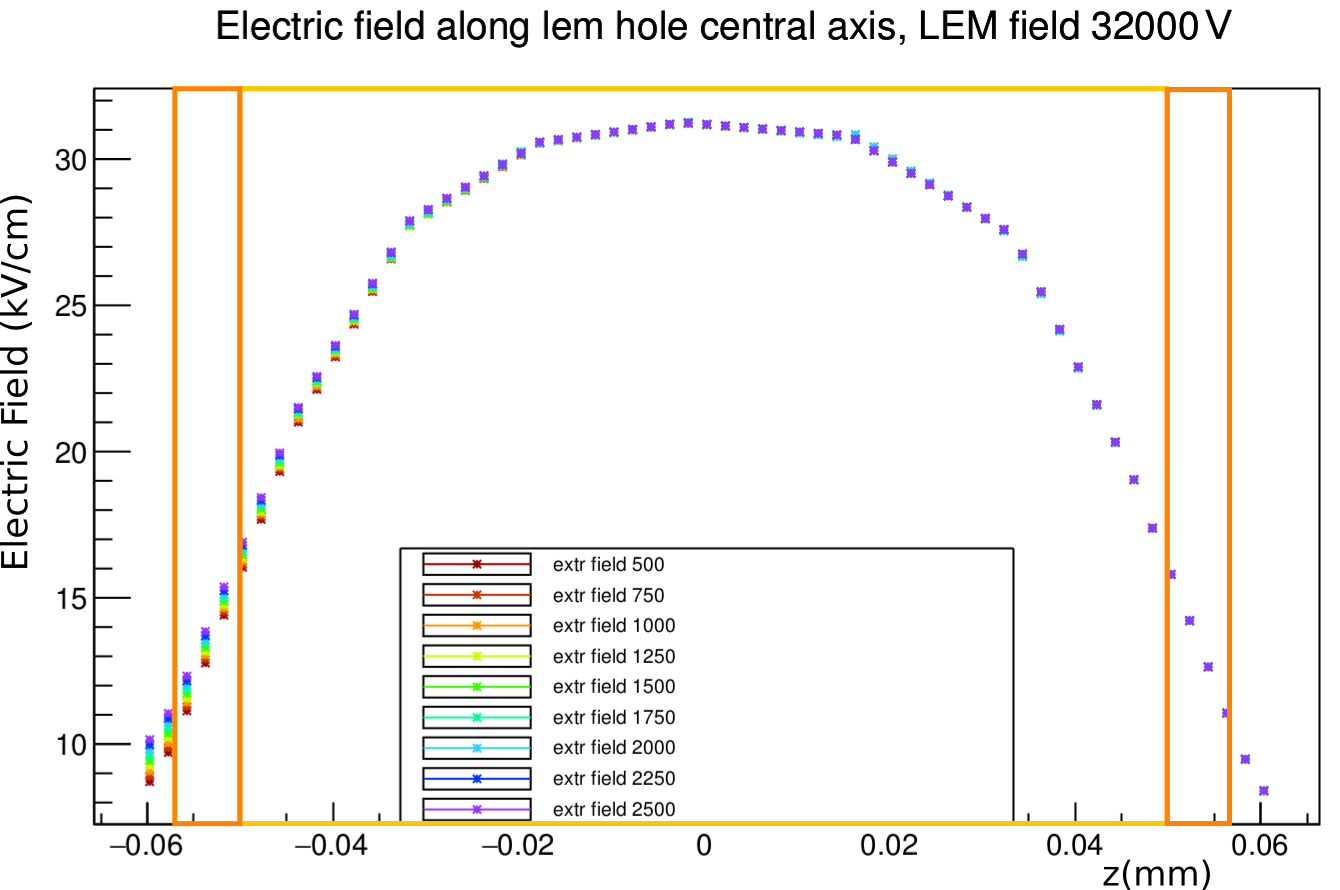
\includegraphics[width=\textwidth,keepaspectratio]{champ_dans_lem_extr.png}
                    \caption{Champ électrique le long de l'axe central d'un trou d'amplification de \gls{lem} pour un champ d'amplification de \SI{32}{\kilo\volt\per\centi\meter} et plusieurs champs d'extraction.}
                    \label{fig::champ_dans_lem_extr}
                \end{subfigure}
                \hfill
                \begin{subfigure}[t]{0.48\textwidth}
                    \includegraphics[width=\textwidth,keepaspectratio]{champ_dans_lem_ind.png}
                    \caption{Champ électrique le long de l'axe central d'un trou d'amplification de \gls{lem} pour un champ d'amplification de \SI{32}{\kilo\volt\per\centi\meter} et plusieurs champs d'induction.}
                    \label{fig::champ_dans_lem_ind}
                \end{subfigure}
                \caption[Influence des variations des champs d'extraction et d'induction sur le champ électrique aux limites du \gls{lem}.]{Influence des variations des champs d'extraction et d'induction sur le champ électrique aux limites du \gls{lem}. Les zones délimitées par les rectangles jaunes et oranges représentent respectivement le \gls{fr4} et les deux épaisseurs de cuivre.}
                \label{fig::champ_dans_lem}
            \end{figure}
        
            Le logiciel de simulation \gls{ansys}, utilisant la méthode des éléments finis, a été utilisé pour générer les cartes de champs de la zone entre la grille d'extraction et l'anode (voir \autoref{fig::ansys_geom}), pour plusieurs configuration de champs électriques. La supposition est faite que le la probabilité de collection d'extraction n'aura aucune influence sur la probabilité de collection d'induction. En revanche, le champ d'amplification peut avoir une influence sur l'une comme sur l'autre. En effet, la valeur du champ électrique à l'entrée ou à la sortie du \gls{lem} va être influencée par la valeur du voltage à travers le \gls{lem} comme le montre les profiles du champ électrique dans le \gls{lem} pour différents champs d'amplification (voir \autoref{fig::champ_dans_lem}). Il a donc été décidé de simuler la probabilité de collection d'extraction(d'induction) contre le champ d'amplification et le champ d'extraction(d'induction) contre le champ d'amplification.\\
            
            Le terme \textit{champ d'extraction} sera employé pour désigner la quantité correspondant à la différence de potentielle entre la grille et le bas du \gls{lem} divisée par la distance entre les deux. Cette zone étant l'interface liquide/gaz, la valeur en question ne correspond ni au champ dans le liquide ni au champ dans le gaz, mais elle est plus pratique à utiliser que la différence de potentielle. Par exemple, un \textit{champ d'extraction} de $\SI{2.5}{\kilo\volt\per\centi\meter}$ correspond à environ $\SI{2}{\kilo\volt\per\centi\meter}$ dans le gaz et $\SI{3}{\kilo\volt\per\centi\meter}$ dans le liquide. Cette ambiguïté n'existe pas pour le champ d'induction, qui n'est que dans le gaz avec une constante diélectrique très proche de l'unité.\\
            
            Le logiciel GarField a été ensuite utilisé pour simuler la dérive d'électrons dans la phase gazeuse. Un grand nombre d'électrons\footnote{De l'ordre de \numprint{10000}} est généré selon une distribution uniforme juste au dessus de la phase gazeuse, avec une énergie initiale nulle, afin de s'affranchir de l'efficacité d'extraction, impossible à simuler avec GarField. Le logiciel effectue alors le transport de ces électrons dans la carte de champ (voir \cite{garfield}) ainsi que l'amplification dans les trous du \gls{lem}. Les positions de début et de fin de parcours de chaque électrons sont enregistrées. La \autoref{fig::drift_histograms} montre la distribution de ces positions.\\
            
            %TODO refaire les histo qui sont moches (drift_histograms) et les efficacités
            
            Il y a alors deux possibilités pour définir les probabilités de collection. La première consiste à trouver les limites effectives de la zone d'amplification, qui est donnée par la simulation comme la région dans laquelle, à l'intérieur des \glspl{lem}, des électrons apparaissent. La probabilité de collection d'extraction est alors définie comme le complémentaire du rapport du nombre d'électrons qui meurent avant la zone d'amplification sur le nombre d'électrons générés au départ. La probabilité de collection d'induction quant à elle est définie comme le complémentaire du rapport du nombre d'électrons qui meurent entre le début de la zone d'amplification et l'anode sur le nombre d'électrons qui sont entrés ou ont été générés dans la zone d'amplification. Cette définition peut correspondre à des probabilités de collection avant que le \gls{lem} ne se charge, donc en début d'exploitation d'un détecteur. Mais une fois chargé, on s'attend à ce que moins de charge meurent dans les trous du \gls{lem}.\\
            
            Une autre manière de définir les probabilités de collection est de considérer qu'un électron est effectivement extrait dès qu'il passe le cuivre bas, et qu'il a effectivement quitté le \gls{lem} si il meure après le cuivre haut. Ici aussi, le résultat peut être différent après charge du \gls{lem}. Un approfondissement de ces simulations serait de prendre cette charge en compte, en réalisant plusieurs itérations de la méthode décrite plus haut en mettant à jours la carte de champ entre chaque itération pour prendre en compte les électrons à présent accrochés au \gls{lem}.\\
            
            
            
        \subsection{Mesures à Saclay avec des LEM et anodes de \texorpdfstring{$10\times\SI{10}{\cm\squared}$}{10x10cm2} }
        
        \subsection{Résultats et comparaison aux expériences passées}